\documentclass{article}
\usepackage{amsmath, amsthm, amssymb, amsfonts, mathtools,enumitem, stmaryrd,physics, cancel, tikz-cd, graphicx, float, booktabs, xurl}
\usetikzlibrary{arrows}
\usepackage{geometry}
    \geometry{
        a4paper,
        left = 40mm,
        top = 20mm,
        right = 40mm,
        bottom = 30mm
    }
\setlength{\parindent}{0pt}
\setlength{\parskip}{\baselineskip}%

\theoremstyle{definition}
\newtheorem{problem}{Problem}
\newtheorem{solution}{Solution}
\newtheorem*{example}{Example}
\newtheorem*{exercise}{Exercise}
\newtheorem*{definition}{Definition}
\newtheorem{theorem}{Theorem}
\newtheorem*{theorem*}{Theorem}
\newtheorem{proposition}[theorem]{Proposition}
\newtheorem*{proposition*}{Proposition}
\newtheorem{lemma}[theorem]{Lemma}
\newtheorem*{lemma*}{Lemma}
\newtheorem{corollary}[theorem]{Corollary}
\newtheorem*{corollary*}{Corollary}
\newtheorem*{remark}{Remark}

\title{M633 Algebraic Varities I}
\author{Thanic Nur Samin}
\date{}

\begin{document}
    \maketitle

    \section*{Monday, 8/25/2025}
    
    Textbook: The Rising Sea.
    
    Link: \url{https://math.stanford.edu/~vakil/216blog/FOAGjul2724public.pdf}

    Office Hours: Wednesdays 4-5, Fridays 1-2

    It's basically an introduction to the scheme point of view for algebraic geometry.

    Grothendieck POV: if we get the definitions right, hard problems will become easier. We are trying to get the definition here.

    \section*{Motivation / A Pseudo History}

    Let \(X\) be a topological space (Compact, Hausdorff).

    \(C(X)=\) ring of real-valued continuous functions.

    Question: What are the maximal ideals of \(C(X)\)?

    Fact: TFAE: given a ring \(A\),

    \begin{enumerate}[label=\roman*)]
        \item \(I\) is maximal among proper ideals of \(A\)
        \item \(A / I\) is a field
        \item There exists a surjective homomorphism from \(A\) to a field \(F\), \(\phi : A \to F\) such that \(I = \ker \phi\)  
    \end{enumerate} 

    If \(x_0\in X\), we have the ring homomorphism \(\operatorname{eval}_{x_0}: f \mapsto f(x_0)\).

    This is an \(\mathbb{R}\)-linear map.

    This is also obviously surjective.

    Thus, \(\ker \operatorname{eval}_{x_0} = \left\{ f\in C(x) \mid f(x_0) = 0 \right\}\). This is a maximal ideal. In fact,

    \begin{theorem}
        All maximal ideals of \(C(X)\) are of the form \(\ker \operatorname{eval}_{x_0}\).
    \end{theorem}

    \begin{proof}
        Suppose not. Let \(\phi : C(X) \to F\) be a surjective homomorphism to a field, and let \((f_1, f_2, f_3, \cdots) = \ker \phi\).
        
        If \(\ker \phi \neq \ker \operatorname{eval}_{x_0} \implies \exists f_{x_0}\in \ker \phi\) such that \(f_{x_0}(x_0)\neq 0\). This is true for each point \(x_0\in X\).

        Therefore, \(f_{x_0}(x)\neq 0\) for all \(x\in U_{x_0}\) where \(U_{x_0}\) is an open neighborhood of \(x_0\).

        Since \(X\) is compact, there is \(x_1, \cdots , x_n \in X\) so that \(U_{x_j}\) cover \(x\).

        \(f_1, \cdots , f_n \in \ker \phi\) such that \(f_i(x) \neq 0 \forall x\in U_{x_i}\).

        Then \(f(x) \coloneqq \sum_{i} f_i^2(x) > 0\) for all \(x\in X\). Then \(\frac{1}{f}\in C(X) \implies 1\in \ker \phi\). Contradiction!  
    \end{proof}

    Given \(f\in C(X)\) define \(Z(f) = f ^{-1} (0)\). This is a closed subset of \(X\).
    
    We can do abuse of notation and say \(X = \operatorname{Max}(C(X))\).

    Then \(Z(f) = \left\{ \mathfrak{m} \in \operatorname{Max} (C(X)) \mid f\in \mathfrak{m} \right\} \) 

    Then, \(Z(f)^c\) open in \(X\)

    \(= \left\{ \mathfrak{m} \in \operatorname{Max} (C(X)) \mid f\notin \mathfrak{m} \right\} \) 

    We have successfully turned a topological space into a ring.

    If we have \(X \xrightarrow{cont} Y\) we have \(C(Y) \to C(X)\).

    Instead of arbitrary topological spaces, now we focus on \(\mathbb{C}^n\).

    Lets look at polynomials \(\mathbb{C}^n \to \mathbb{C}\).

    Ring of polynomial functions is \(\mathbb{C} [x_1, \cdots , x_n]\).

    \begin{theorem}
        [Weak Hilbert Nullstellensatz] Maximal ideals of this ring are exactly the kernels of evaluation maps at points \((a_1, \cdots , a_n) \in \mathbb{C}^n\).
    \end{theorem}

    Note that \(x_1 - a_1, \cdots , x_n - a_n\in \ker \operatorname{eval}_{(a_1, \cdots , a_n)}\). In fact, \(\ker \operatorname{eval}_{(a_1, \cdots , a_n)} = (x_1 - a_1, \cdots , x_n - a_n)\).

    \begin{proof}
        WLOG \(a_1 = \cdots = a_n = 0\). Then \(\ker \operatorname{eval}_{(0,\cdots ,0)}\) are exactly the polynomial with no constant term, which is exactly \((x_1, \cdots , x_n)\).
    \end{proof}

    Now we prove weak Nullstellensatz.

    \begin{proof}
        Let \(\mathfrak{m} \subset \mathbb{C} [x_1, \cdots , x_n]\) be a maximal ideal. Then \(F = \mathbb{C}[x_1, \cdots , x_n] / \mathfrak{m}\) is a field extension of \(\mathbb{C}\). So, \(F\) is transcendental. Choose \(x\in F \setminus \mathbb{C}\). Then \(x\) generates a subfield \(\mathbb{C} (x)\).

        Then, \(\dim _{\mathbb{C} \text{-v.s.}} \mathbb{C}(x)\) is uncountable. To prove this, note that \(\left\{ \frac{1}{x-c} \mid c\in \mathbb{C} \right\}\) are linearly independent.
        
        However, \(\dim_{\mathbb{C}\text{-v.s.}} \mathbb{C}[x_1, \cdots, x_n]\) is countable. 
    \end{proof}

    Given a system of polynomial equations:

    \(f_1 (x_1, \cdots , x_n) = 0\)
    
    \(\vdots\)
    
    \(f_m(x_1, \cdots , x_n) = 0\) 

    Find or describe the set of complex solutions.

    We want to find all \(\mathfrak{m} \in \operatorname{Max} (\mathbb{C} [x_1, \cdots , x_n])\) such that \(f_1, \cdots , f_m \in \mathfrak{m}\).

    Define \(I = (f_1, \cdots , f_m)\). Then, we want \(\{ \mathfrak{m} \mid I \subset \mathfrak{m} \}\).

    We have turned the problem of finding solutions to finding maximal ideal containing a certain ideal.

    From the theorem about order preserving bijection of ideal containing ideal and quotient,

    We want all maximal ideals \(\overline{\mathfrak{m}}\) in \(\mathbb{C} [x_1, \cdots , x_n] / I\).

    We want to do the most general thing. There is nothing special about polynomials!

    Let \(A\) be a commutative ring.  We think of \(\operatorname{Max}(A)\) as the associated space.

    \textbf{If somebody gives us a ring \(A\), we want to think of it as a ring of function on a space. \(\operatorname{Max}(A)\) is that space.}

    There is a problem with this idea: We would like to be able to go from \(\operatorname{Max}(A) \to \operatorname{Max}(B)\) whenever we have a ring homomorphism \(f: B \to A\).

    Suppose \(\mathfrak{m} \subset A\). We want t have \(f ^{-1} (\mathfrak{m})\). We want this to be maximal. It is not always maximal!
    
    Suppose we have a homomorphism \(\mathbb{C} [x] \hookrightarrow \mathbb{C} (x)\).

    There is only one maximal ideal on \(\mathbb{C}(x)\). It is \((0)\). Then \(f ^{-1} ((0)) = (0)\) but \((0)\) is not a maximal ideal in \(\mathbb{C}[x]\).

    The solution is to not use \(\operatorname{Max}(A)\), but rather \(\operatorname{Prime}(A)\).

    Let \(f: B \to A\) be a homomorphism and let \(P \subset A\) be a prime ideal.

    Claim: \(f^{-1} (P)\) is also prime.

    Proof: \(xy\in f ^{-1} (P) \implies f(xy)\in P \implies f(x)f(y)\in P \implies f(x) \in P \lor f(y)\in P \implies x\in f ^{-1} (P) \lor y\in f ^{-1} (P)\).

    This works! But how does this mess up the space? What additional points do we have?

    \section*{Wednesday, 8/27/2025}
    
    Now we go back to the textbook.

    We start with some category theory. For this course, categories will be locally small. The objects might not be sets, but hom-sets will be sets.

    Let \(\mathcal{C}, D\mathcal{C}\) be categories. \(\mathcal{C} \xrightarrow{F} \mathcal{D}\) morphisms.

    Let \(F: \operatorname{ob} \mathcal{C} \to \operatorname{ob} \mathcal{D}\).

    Suppose \(X,Y\in \operatorname{ob} \mathcal{C}\).

    \(\phi: X \to Y\) means \(\phi \in \operatorname{Mor}_{\mathcal{C}}(X,Y)\).
    
    Then, \(F(\phi): F(X) \to F(Y), F(\phi)\in \operatorname{Mor}_{\mathcal{D}}(F(X),F(Y))\). 

    We have the following categories: Sets, Groups, Ab, Top, Rings, Comm, Field, \(R\)-mod, COmplexes of \(R\)-mod, Sheaves on \(X\), etc.

    \begin{definition}
        A functor is \textit{faithful} if \(\forall X,Y\in \operatorname{Ob} \mathcal{C}, \operatorname{Mor}_{\mathcal{C}} (X,Y) \to \operatorname{Mor}_{\mathcal{D}}(F(X),F(Y))\) is injective.

        It is \textit{fully faithful} if this map is a bijection.
    \end{definition}

    \(\operatorname{Top} ^{\ast} =\) category of pointed topological spaces. This contains pairs \((X,x)\), space with a point.
    
    \(\operatorname{Mor}_{\operatorname{Top}^{\ast}}\left( (X,x),(Y,y) \right) = \left\{ \text{cont. maps } f: X\to Y \text{ s.t. } f(x) = y \right\}\)

    This is useful: we can't find fundamental group without a base point.

    Then, \(\pi_1\) is a functor from \(\operatorname{Top}^{\ast}\) to Groups. Morphism \((X,x) \xrightarrow{f} (Y,y)\) gives us \(f_{\ast} : \pi_1(X,x) \to \pi_1(Y,y)\) which is a group homomorphism.

    We want to talk about natural transformation which is important for this course.

    \begin{definition}
        [Natural Transformation] Consider functors \(\mathfrak{f},\mathfrak{g}: \mathcal{C} \to \mathcal{D}\).

        A natural transformation \(T: \mathfrak{f} \to \mathfrak{g}\) assigns to each \(x \in \operatorname{ob} \mathcal{C}\) an element \(T(x) \in \operatorname{Mor}_{\mathcal{D}} (\mathfrak{f}(x), \mathfrak{g}(x))\) with compatibilty condition:

        Given \(x,y\in \operatorname{Ob} (\mathcal{C}), f\in \operatorname{Mor}_{\mathcal{C}}(x,y)\) such that the following diagram commutes:

        \[
            \begin{tikzcd}
                \mathfrak{f} (x) \ar[r,"T(x)"] \ar[d,"\mathfrak{f}(f)"'] & \mathfrak{g}(x) \ar[d,"\mathfrak{g}(f)"] \\ \mathfrak{f}(y) \ar[r,"T(y)"] & \mathfrak{g}(y) 
            \end{tikzcd}
        \]
    \end{definition}

    
    \begin{definition}
        If \(f\in \operatorname{Mor}_{\mathcal{C}}(x,y), g\in \operatorname{Mor}_{\mathcal{C}}(y,x)\) we say \(f\) and \(g\) are inverses iff \(f \circ g = \operatorname{id}_{y}, g \circ f = \operatorname{id}_{x}\).

        A morphism which has an inverse is called an isomorphism.
    \end{definition}
    
    Inverses are unique. If \(h\) is also an inverse of \(f\) then \(h \circ f \circ g = h \circ (f \circ g) = h \circ \operatorname{id}_{y} = h\) and \(h \circ f \circ  g= (h \circ f) \circ  g = \operatorname{id}_{x} \circ  g = g\).

    \begin{definition}
        Morphisms with inverses are isomorphisms.
    \end{definition}

    \begin{definition}
        A category in which every morphism has an inverse is called a groupoid.
    \end{definition}

    Lets talk about an example. Consider the cateory with \(1\) object \(\{ \ast \}\). Since our categories are locally small, the morphisms form a set. There is a composition law. This gives us:

    \textit{A category with one object is a monoid}.

    Of course, if we add the stipulation that every morphism must have an inverse,

    \textit{A groupoid with one object is a group}.

    We want a categorical analogue for injectivity and bijectivity. Consider the example of the same set with two topologies, one finer than the other. Then on the point level we can have a bijection, but one map is continuous and the inverse map is not.

    This gives us the concepts of monomorphism and epimorphism.

    Monomorphism loosely resembles injectivity.

    Epimorphism loosely resembles surjectivity.

    \begin{definition}
        \(f \in \operatorname{Mor}_{\mathcal{C}}(x,y)\) is a \textit{monomorphism} if \(\forall z\in \operatorname{Ob} \mathcal{C}\) and all \(g,h\in \operatorname{Mor}_{\mathcal{C}}(z,x)\) we have:
        
        \[
            f \circ  g = f \circ h \implies g = h
        \]

        \[
            \begin{tikzcd}
                z \ar[r, shift left = 2pt, "g"] \ar[r, shift right = 2pt, "h"'] & x \ar[r,"f"] & y
            \end{tikzcd}
        \]
    \end{definition}

    \begin{definition}
        \(f \in \operatorname{Mor}_{\mathcal{C}}(x,y)\) is epimorphic if \(\forall z\in \operatorname{Ob}\mathcal{C}, \forall g,h\in \operatorname{Mor}_{\mathcal{C}}(y,z)\),
        
        \[
            g \circ f = h \circ  f \implies g = h
        \]

        \[
            \begin{tikzcd}
                x \ar[r,"f"] & y \ar[r, shift left = 2pt, "g"] \ar[r, shift right = 2pt, "h"'] & z
            \end{tikzcd}
        \]
    \end{definition} 

    \begin{definition}
        [Natural Isomorphism] Given categories \(\mathcal{C}\) and \(\mathcal{D}\) and a functor \(\mathfrak{f}, \mathfrak{g}: \mathcal{C} \to \mathcal{D}\), a natural isomorphism is a natural transformation \(T\) from \(\mathfrak{f}\) to \(\mathfrak{g}\) such that for all \(x\in \operatorname{Ob} \mathcal{C}\),

        \[
            T(x) \in \operatorname{Mor}_{\mathcal{D}}(\mathfrak{f}(x), \mathfrak{g} (x))
        \]

        is an isomorphism.
    \end{definition}

    Nonexample of natural isomorphism: fix a field \(k\) and let \(C = \operatorname{Vect}_k\). Consider the double dual functor \(f: \mathcal{C} \to \mathcal{C}\) so that \(V \to (V^{\ast})^{\ast}\).

    [We take two duals since only one would mean this is a contravariant functor. We want the direction of the functors to be the same].

    Consider the identity functor \(\operatorname{id}_{\mathcal{C}}: V \to V\).
    
    We have a natural transformation \(\operatorname{id}_{\operatorname{Vect}_k} \to \mathfrak{f}\) by \(V \mapsto (V \to V^{\ast})\)
    
    Any \(v\in V\) defines a linear transformation \(T_v : V^{\ast} \to k\) given by \(T_v(v^{\ast}) = v^{\ast} (v)\). Then \(T_v \in (V^{\ast})^{\ast} = V^{\ast\ast}\).
    
    We have the following commutative diagram:

    \[
        \begin{tikzcd}
            V \ar[r,"T_v"] \ar[d,"A"] & V^{\ast\ast} \ar[d,"T(A)"] \\ W \ar[r,"T_w"] & W^{\ast\ast} 
        \end{tikzcd}
    \]

    If \(V\) is infinite dimensional, then \(\dim V^{\ast} > \dim V\). Then \(\dim V^{\ast\ast} > \dim V\). So this is only a natural transformation, not a natural isomorphism.

    Note that however in \(\operatorname{Vect}_k^{\text{fin}}\) the double dual is a natural isomorphism.

    Also see: equivalence of categories.

    \section*{Friday, 8/29/2025}
    
    We continue category theory today.

    \begin{definition}
        [Equivalence of Categories] If \(\mathcal{C}\) and \(\mathcal{D}\) are categories and \(F: \mathcal{C} \to \mathcal{D}\) and \(G: \mathcal{D} \to \mathcal{C}\) are functors such that \(F \circ G : \mathcal{D} \to \mathcal{D}\) and \(G \circ F: \mathcal{C} \to \mathcal{C}\) are naturally isomorphic to \(\operatorname{id}_{\mathcal{D}} \) and \(\operatorname{id}_{\mathcal{C}} \) respectively.
    \end{definition}

    For example, let \(\mathcal{C} =\) category with objects \(\varnothing , \{ 1 \} , \{ 1,2 \}, \{ 1,2,3 \}, \cdots\) and morphisms are functions.

    Let \(\mathcal{D}\) be the category of finite sets and morphisms are functions.

    We have an obvious functor: \(\mathcal{C} \to \mathcal{D}\) sends each \(\{ 1, 2, \cdots , n \} \) to itself.

    For \(\mathcal{D} \to \mathcal{C}\) we need to work a little bit harder, and we have to deal with axiom of choice and other stuff. To avoid these, we introduce the following easier definition:

    \begin{definition}
        If \(\mathcal{C}\) and \(\mathcal{D}\) are categories and \(F: \mathcal{C} \to \mathcal{D}\) and:

        \begin{enumerate}[label=\arabic*)]
            \item \(F\) is fully faithful
            \item \(F\) is essentially surjective. 
        \end{enumerate} 

        [Essentially surjective means every object is isomorphic to an object in the image. Every set with \(n\) elements is isomorphic to \(\{ 1,\cdots ,n \}\) for example.]

        Then \(\mathcal{C}\) and \(\mathcal{D}\) are equivalent.
    \end{definition}

    Given a category \(\mathcal{C}\) and \(A \in \operatorname{ob} \mathcal{C}\) we define functors:

    \(h_A: \mathcal{C} \to \operatorname{Sets}\) given by \(h_A(X) = \operatorname{Mor}_{\mathcal{C}} (A,X)\). This is contravariant.

    \(h^A: \mathcal{C} \to \operatorname{Sets}\) given by \(h^A(X) = \operatorname{Mor}_{\mathcal{C}} (X,A)\)

    Given \(A,B \in \operatorname{Ob} \mathcal{C}, \phi \in \operatorname{Mor}_{\mathcal{C}} (A,B)\), \(\phi\) deines a functor \(h_B(X) \to h_A(X)\) and \(h^A(X) \to h^B(X)\).

    \begin{definition}
        A contravariant functor \(F: \mathcal{C} \to \operatorname{Sets}\) is \textit{representable} if \(\exists A \in \operatorname{Ob} \mathcal{C}\) such that \(F = h_A\).
    \end{definition}

    \begin{theorem}
        [Yoneda Lemma] The set of natural transformations \(h_A \to h_B\) is naturally isomorphic to \(\operatorname{Mor}_{\mathcal{C}}(B,A)\).
    \end{theorem}

    \begin{proof}
        Let \(N\) be a natural transformation from \(h_A\) to \(h_B\). i.e. for \(X\in \operatorname{ob} \mathcal{C}\) we have:

        \[
            N(X) : \underset{= \operatorname{Mor}_{\mathcal{C}} (A,X)}{h_A(X)} \to \underset{=\operatorname{Mor}_{\mathcal{C}} (B,X)}{h_B(X)}  
        \]

        Let \(X = A\). Then, \(N(A): h_A(A) \to h_B(A) \implies N(A): \operatorname{Mor}_{\mathcal{C}} (A,A) \to \operatorname{Mor}_{\mathcal{C}} (B,A)\)
        
        Let \(N(A)(\operatorname{id}_{A})\eqqcolon \psi\).
        
        Composition by \(\psi\) gives a map \(h_A \to h_B\), i.e. for all \(Y\in \operatorname{Ob} \mathcal{C}\), composition by \(\psi\) gives \(h_A(Y) \to h_B(Y)\) which is the same as \(N(Y)\).

        Let \(f: X \to Y\). We have:

        \[
            \begin{tikzcd}
                \operatorname{Mor}_{\mathcal{C}} (A,X) \ar[r,"N(X)"] \ar[d,"f_{\ast}"] & \operatorname{Mor}(B,X) \ar[d,"f_{\ast}"] \\ \operatorname{Mor}(A,Y) \ar[r,"N(Y)"] & \operatorname{Mor}(B,Y)
            \end{tikzcd}
        \]

        Setting \(X = A\),

        \[
            \begin{tikzcd}
                \operatorname{Mor}_{\mathcal{C}} (A,A) \ar[r,"N(X)"] \ar[d,"f_{\ast}"] & \operatorname{Mor}(B,A) \ar[d,"f_{\ast}"] \\ \operatorname{Mor}(A,Y) \ar[r,"N(Y)"] & \operatorname{Mor}(B,Y)
            \end{tikzcd}
        \]

        taking \(\operatorname{id}_{A}\) and applying the commutativity,

        \[
            \begin{tikzcd}
                \operatorname{id}_{A} \ar[r,"N(X)"] \ar[d,"f_{\ast}"] & \psi \ar[d] \\ f \ar[r] & N(Y)(f) = f \circ \psi  
            \end{tikzcd}
        \]
    \end{proof}

    \subsection*{Universal Objects}

    \begin{definition}
        An object \(X\in \operatorname{ob} \mathcal{C}\) is an \textit{initial object} if \(\forall Y\in \operatorname{ob} \mathcal{C}, \vert \operatorname{Mor}_{\mathcal{C}} (X,Y) \vert = 1\).

        It is a final object if \(\forall Y\in \operatorname{ob} \mathcal{C}, \vert \operatorname{Mor}_{\mathcal{C}} (Y,X) \vert = 1\). 
    \end{definition}

    Up to \textit{unique isomorphism} an initial or final object in a category is unique if it exists.

    \begin{definition}
        Let \(L\) be a (commutative) ring and \(S\) a multiplicative system in \(A\), meaning \(1\in S, x,y\in S \implies xy\in S, 0\notin S\).

        The localization \(S ^{-1} A\) is the \textit{universal \(A\)-algebra in which every element of \(S\) is invertible.}

        \(\frac{a_1}{s_1} = \frac{a_2}{s_2}\) means \((a_1 s_2 - a_2 s_1) s_3 = 0\) for some \(s_3 \in S\).
    \end{definition}

    We need the construction to show that the localization exists. But it is easier to work with the universal property!

    \(S ^{-1} A\), assuming it exists, is universal among all \(A\)-algebras in which \(S\) is invertible.

    Consider all ring homomorphisms \(\left\{ \phi : A \to B \mid \phi(s) \text{ is a unit in \(B\) for all \(s\in S\)} \right\} \) 

    We can now define a category. Let this set be \(\operatorname{ob} \mathcal{C}\). Let the morphisms be as follows:

    \[
        \begin{tikzcd}
            & B \ar[dd]\\ A \ar[ru,"\phi"] \ar[rd,"\psi"] \\ & C
        \end{tikzcd}
    \]

    Existence of \(S ^{-1} A\) is expressed by the existence of an initial object in this category.

    We have the homomorphism \(A \to S ^{-1} A\) by \(a \mapsto \frac{a}{1}\).

    \[
        \begin{tikzcd}
            & S ^{-1} A \ar[dd, dotted, "!"]\\ A \ar[ru] \ar[rd,"s \mapsto b^{\ast}"] \\ & B
        \end{tikzcd}
    \]

    Another example: suppose \(A\) is a ring and \(M,N\) are \(A\)-modules. We can define tensor product \(M \otimes_A N\).

    The property we're interested in is: \(\operatorname{Hom}_A (M \otimes_A N, X) = A \text{-billinear}(M \times N, X)\). 

    Fix \(M,N\). Consider the functor \(X \mapsto \left\{ A \text{-billinear maps } M \times N \to X \right\}\).

    This functor is \textit{representable} by in the category of \(A\)-modules.

    \[
        \begin{tikzcd}
            & M \otimes_A N \ar[rd,dotted, "!"] \\ M \times N \ar[rr] \ar[ur] && X
        \end{tikzcd}
    \]

    Does (Sets) have an initial and final object? \(\varnothing\) is initial, any \(1\)-element set is final.

    What about the category of complex vector spaces?

    \(0\) is initial and final.

    A zero object is an object that is both initial and final.

    Category of infinite sets doesn't have an initial or final object.

    In the category of rings, \(\mathbb{Z} \to R\) always exists so it's initial. We don't take zero rings so there's no final object.

    Note that if we have a map of rings \(A \to B\), the map of schemes go in the opposite direction: \(\operatorname{Spec} B \to \operatorname{Spec} A\). So there should be a final object in the category of schemes.

    \section*{Wednesday, 9/3/2025}
    
    \subsection*{Products and Coproducts}

    Suppose we have a category \(\mathcal{C}\), index set \(I\) and for each \(\alpha \in I\) we have \(X_\alpha \in \operatorname{ob} \mathcal{C}\).

    We want to talk (in a categorical sense) about the product of all the \(X_\alpha\)'s. This should be analogous to the cartesian product, we should be able to extract the initial object.

    The product, thus, should be an object \(X\in \operatorname{ob} \mathcal{C}\) together with the maps \(\pi_\alpha \in \operatorname{Mor}_{\mathcal{C}} (X,X_\alpha)\) which is universal for such data.

    For example, in the case \(I = \{ 1,2 \}\) and \(X = X_1 \times X_2\), \(X\) is universal in the following sense:

    \[
        \begin{tikzcd}
            & Y \ar[ldd, bend right] \ar[rdd, bend left] \ar[d, dotted] \\ & X \ar[ld] \ar[rd] \\ X_1 & & X_2
        \end{tikzcd}
    \]

    For coproducts we just reverse the arrows.

    Category \(\mathcal{C}, \alpha \in I\) index set, \(X_\alpha \in \operatorname{ob} \mathcal{C}\).
    
    The coproduct \(\coprod_\alpha X_\alpha\) of the \(X_\alpha\)'s is an object \(X\in \operatorname{ob} \mathcal{C}\) together with maps \(i_\alpha \in \operatorname{Mor}_{\mathcal{C}} (X_\alpha , X)\) with is universal for such data. For \(I = \{ 1,2 \}\) and \(X = X_1 \coprod X_2\):

    \[
        \begin{tikzcd}
            & Y & \\ & X \ar[u, dotted] \\ X_1 \ar[uur, bend left] \ar[ur] & & X_2 \ar[uul, bend right] \ar[ul]
        \end{tikzcd}
    \]

    In the category of sets, product is the cartesian product, and coproduct is the disjoint union.

    In \(\operatorname{Ab}\), the product and coproduct of two objects are the same, the direct sum as long as the index set is finite.

    For infinite index set,

    \(\coprod_{i=1}^{\infty} = \bigoplus_{i=1}^{\infty} X_i = \left\{ (x_1, x_2, \cdots ) \mid x_i \in X_i, x_i = 0 \, \forall i \gg 0 \right\}\)
    
    Finite sums.

    \(\prod_{i=1}^{\infty} X_i = \left\{ (x_1, x_2, \cdots ) \mid x_i\in X_i \right\} \)
    
    Unrestricted.

    These are not the same! Infinite product of \(\mathbb{Z}\) is not free for example.

    We can write it like this:

    \(\operatorname{Ab} \times \operatorname{Ab} \xrightarrow{\coprod} \operatorname{Ab}\) 

    \(\operatorname{Ab} \times \operatorname{Ab} \xrightarrow{\prod} \operatorname{Ab}\)

    We have the following natural transformation:

    \((X_1, X_2) \mapsto \begin{matrix} (X_1 \oplus X_2 \to X_1 \times X_2) \\ (x_1, x_2) \mapsto (x_1, x_2) \end{matrix}\) 

    Something that is both a product and a coproduct is called a biproduct.

    \subsection*{Limits and Colimits}

    We can generalize the concepts of product to limit and coproduct to colimit.

    Limits/Colimits are the \textit{same thing} but instead of an index set \(I\) we use an \textit{index category} \(\mathcal{I}\).

    The data which determines the limit/colimit is a functor from \(\mathcal{I} \to \mathcal{C}\).

    For example: consider the following category of \(3\) elements (ignore the identity morphisms):

    \[
        \begin{tikzcd}
            1 \ar[d] \\ 0 & 2 \ar[l]
        \end{tikzcd}
    \]

    Consider functors from this category to a category \(\mathcal{C}\). We then have the following in \(\mathcal{C}\):

    \[
        \begin{tikzcd}
            X_1 \ar[d] \\ X_0 & X_2\ar[l]
        \end{tikzcd}
    \]

    The limit of such a diagram, if it exists consists of \(X\in \operatorname{ob} \mathcal{C}\) and maps \(\pi_i \in \operatorname{Mor}_{\mathcal{C}}(X,X_i)\) such that the diagram:

    \[
        \begin{tikzcd}
            X_1 \ar[d] & X \ar[l] \ar[ld] \ar[d] \\ X_0 & X_2\ar[l]
        \end{tikzcd}
    \]

    commutes with the universal property:

    \[
        \begin{tikzcd}
            & & Y \ar[dll] \ar[ddl] \ar[dl, dotted] \\ X_1 \ar[d, "f_1"] & X \ar[l] \ar[ld] \ar[d] \\ X_0 & X_2\ar[l, "f_2"]
        \end{tikzcd}
    \]

    This is specific case is called the fiber product.

    In (Sets) all limits and colimits exist.

    In the fiber product example, we can consider \(X = \coprod_{x_0\in X_0} f_1 ^{-1} (x_0) \times f_2 ^{-1} (x_0)\).

    We can look at the following category of natural number: \(\mathcal{I} \coloneqq \cdots \to 4 \to 3 \to 2 \to 1\) [we don't write arrows \(4 \to 1\) since it's a composition].

    Let \(\mathcal{C} = \operatorname{Ab}\). We can consider \(\mathcal{I} \to \operatorname{Ab}\) so that we have \(\cdots \to X_4 \to X_3 \to X_2 \to X_1\).
    
    Then taking limit gives us the projective limit \(\varprojlim_n X_n\).

    For example if \(X_i = \mathbb{Z} / p^i \mathbb{Z}_i\).

    We have \(\mathbb{Z} / p^{i+1} \mathbb{Z} \to \mathbb{Z} / p^i \mathbb{Z}\) by taking \(\mod p^i\). 

    Then \(\varprojlim_n \mathbb{Z} / p^n\mathbb{Z} = \mathbb{Z}_p = a_0 + a_1 p + a_2 p^2 + \cdots\).

    Note: the topology of \(\mathbb{Z}_p\) is important. Individual \(\mathbb{Z} /p^n \mathbb{Z}\) have discrete topology. They're finite and thus compact. The topology of \(\mathbb{Z}_p\) then comes from Tychonoff's theorem.

    \subsection*{Filtered Category}

    A \textit{filtered category} \(\mathcal{I}\) satisfies:

    \begin{enumerate}[label=\arabic*)]
        \item \(\mathcal{I}\) is non-empty.
        \item If \(x,y\in \operatorname{ob} \mathcal{I}\) there exists \(z\in \operatorname{ob} \mathcal{I}\) such that \(\operatorname{Mor}_{\mathcal{C}} (x,z)\neq \varnothing, \operatorname{Mor}_{\mathcal{C}} (y,z)\neq \varnothing\).
        \item If \(x,y\in \operatorname{ob} \mathcal{I}, f,g\in \operatorname{Mor}_{\mathcal{C}} (x,y)\) then \(\exists z\in \operatorname{ob} \mathcal{I}, h\in \operatorname{Mor}_{\mathcal{C}}(y,z)\) such that \(h \circ f = h \circ g\).   
    \end{enumerate} 

    Condition 2 implies given \(x,y\) we can always find \(z\) such that,

    \[
        \begin{tikzcd}
            x \ar[rd] \\ & z \\ y \ar[ru]
        \end{tikzcd}
    \]

    Condition 3 implies given

    \[
        \begin{tikzcd}
            x \ar[r, bend right] \ar[r, bend left] & y
        \end{tikzcd}
    \]

    We can find

    \[
        \begin{tikzcd}
            x \ar[r, bend right] \ar[r, bend left] & y \ar[r] & z
        \end{tikzcd}
    \]

    Advantage of having a filtered category: we can make colimits exist.

    \begin{theorem}
        The category of fields does not have general colimits but it does have \textit{filtered colimits}
    \end{theorem}

    Take a colimit in the category of sets and observe that it has a field structure.

    How do we add up two elements in different fields \(x\) and \(y\)? Take the field \(z\) and add there!

    \subsection*{Adjoint Functors}

    Suppose we have categories \(\mathcal{C}\) and \(\mathcal{D}\) and functors \(F: \mathcal{C} \to \mathcal{D}, G: \mathcal{D} \to \mathcal{C}\). TFAE:
  
    \begin{enumerate}[label=\arabic*)]
        \item \((F,G)\) is an adjoint pair
        \item \(F\) is the left-adjoint of \(G\)
        \item \(G\) is the right-adjoint of \(F\)
    \end{enumerate} 

    All these equate to saying:

    \begin{definition}
        There is a natural isomorphism between the following: \(\operatorname{Mor}_{\mathcal{D}}(F(X), Y)\) and \(\operatorname{Mor}_{\mathcal{C}}(X, G(Y))\). We denote this by \(N(X,Y)\). So \(\operatorname{Mor}_{\mathcal{D}}(F(X),Y) \xrightarrow{N(X,Y)} \operatorname{Mor}_{\mathcal{C}} (X,G(Y))\).
    \end{definition}

    The picture looks like the following: 
    Suppose we have \(X_1 \to X_2\) in \(\mathcal{C}\). 

    \[
        \begin{tikzcd}
            \operatorname{Mor}_{\mathcal{D}}(F(X_1),Y) \ar[r,"{N(X_1,Y)}"] & \operatorname{Mor}_{\mathcal{C}} (X_1, G(Y)) \\ \operatorname{Mor}_{\mathcal{D}}(F(X_2),Y) \ar[r,"{N(X_2,Y)}"] \ar[u,"F(f)^{\ast}"] & \operatorname{Mor}_{\mathcal{C}} (X_2, G(Y)) \ar[u,"f^{\ast}"] 
        \end{tikzcd}
    \]

    \section*{Friday, 9/5/2025}
    
    Consider the following example:

    \(\mathcal{C} = \text{(Sets)}\)
    
    \(\mathcal{D} = \text{(Ab)}\)

    \(G: \mathcal{D} \to \mathcal{C}\) the forgetful functor.

    \(F: \mathcal{C} \to \mathcal{D}\) the free abelian group functor.

    If \(X\) is any set and \(Y\) is any abelian group, then,

    \[
        \operatorname{Hom}(\operatorname{Free}(X), Y) \xrightarrow{\cong} \operatorname{Func} (X,Y)
    \]

    These are adjoint functors.

    Let \(H\) be a commutative ring, and \(M,X,Y\in \operatorname{ob}(A \text{-mod})\). Then,

    \[
        \operatorname{Hom}_A(M \otimes_A X, Y) \xrightarrow{\cong} \operatorname{Hom}_A (X, \operatorname{Hom}_A(M,Y))
    \]

    Here \(F(X)= M \otimes_A X\)
    
    \(G(Y) = \operatorname{Hom}_A (M,Y)\).

    An example from Homological Algebra:

    Abelian Categories. Examole: Abelian groups, \(k\)-vector spaces, \(A\)-modules, left \(R\)-modules, sheaves of abelian groups, \(k\)-vector spaaces with \(G\)-rep, etc.

    There are axioms for abelian categories but you don't really need to remember it.

    Let \(\mathcal{C}\) be an abelian category. We have the following:
    
    \(\operatorname{Mor}_{\mathcal{C}}(X,Y)\) is an abelain group.

    Composition \(\operatorname{Mor}_{\mathcal{C}}(X,Y) \times \operatorname{Mor}_{\mathcal{C}} (Y,Z) \to \operatorname{Mor}_{\mathcal{C}}(X,Z)\) is bilinear.

    The category has a \(0\)-object.

    The category has a biproduct.

    The category has kernels and cokernels.

    Every monomorphism is the kernel of its cokernel.

    Every epimorphism is the cokernel of its kernel.

    Let's unpack what kernel/cokernel means in a categorical sense.

    Consider \(X \xrightarrow{f} Y\). We also have the zero map \(X \xrightarrow{0} Y\).

    Kernel: Let \(K\) be universal in the following:

    \[
        \begin{tikzcd}
            K^{\prime} \ar[d, dotted] \ar[dr] \\
            K \ar[r] & X \ar[r, bend right,"0"] \ar[r, bend left, "f"] & Y 
        \end{tikzcd}
    \]

    Then the kernel is the morphism \(K \to X\).

    Similarly, let C be universal in the following:

    \[
        \begin{tikzcd}
            X \ar[r, bend right, "0"] \ar[r, bend left, "f"] & Y \ar[r] \ar[rd] & C \ar[d, dotted] \\ & & C^{\prime} 
        \end{tikzcd}
    \]

    cokernel is the morphism \(Y \to C\). That is why it makes sense to talk about kernel of cokernel and cokernel of the kernel.

    Most importantly:

    \begin{theorem}
        An abelian category is a category in which diagram chasing works.
    \end{theorem}

    Every abelian category is equivalent to a full subcategory of \(R\)-mod for some ring \(R\).

    Now let's talk about complexes, so we can talk about homological algebra.

    \begin{definition}
        [Complex] A complex is a sequence of objects and morphisms with the rule that composing any two consecutive morphisms gives the \(0\) morphism.
    \end{definition}

    Going up gives you cochain complexes.

    Going down gives you chain complexes.

    Consider the cochain complex:

    \[
        \cdots \xrightarrow{\phi_{n-2}} X^{n-2} \xrightarrow{\phi_{n-1}} X^{n-1} \xrightarrow{\phi_n} X^n \xrightarrow{\phi_{n+1}} X^{n+1} \xrightarrow{\phi_{n+2}} X^{n+2} \to \cdots 
    \]

    We have the following: \(\phi_{n+1} \circ \phi_n = 0\).

    The \textit{cohomology} of this \textit{cochain complex} is \(H^n(X^\bullet) = \ker \phi_{n+1} / \operatorname{im} \phi_n\).

    Consider \(X \to Y\). We have the following:

    \[
        \begin{tikzcd}
            X \ar[rr] \ar[rd,"epi"] & & Y \\ & Z \ar[ur, "mon"]
        \end{tikzcd}
    \]

    Then \(Z \to Y\) is the image.

    \(X \xrightarrow{f} Y \to \operatorname{coker} f \) then \(\operatorname{im} f = \ker (Y \to \operatorname{coker} f)\).
    
    Example of diagram chase:

    Consider the following \textit{exact} complexes: their cohomology is \(0\), with some more morphisms.

    \[
        \begin{tikzcd}
            0 \ar[r] & X^0 \ar[r] \ar[d,"f^0"] & X^1 \ar[r] \ar[d,"f^1"] & X^2 \ar[r] \ar[d,"f^2"] & 0 \\
            0 \ar[r] & Y^0 \ar[r] & Y^1 \ar[r] & Y^2 \ar[r] & 0
        \end{tikzcd}
    \]

    Then we will have the following:

    \[
        \begin{tikzcd}
            0 \ar[r] & \ker f^0 \ar[r] & \ker f^1 \ar[r] & \ker f^2 \ar[dddll, bend left] \\
            0 \ar[r] & X^0 \ar[r] \ar[d,"f^0"] & X^1 \ar[r] \ar[d,"f^1"] & X^2 \ar[r] \ar[d,"f^2"] & 0 \\
            0 \ar[r] & Y^0 \ar[r] & Y^1 \ar[r] & Y^2 \ar[r] & 0 \\
            & \operatorname{coker} f^0 \ar[r] & \operatorname{coker} f^1 \ar[r] & \operatorname{coker} f^2 
        \end{tikzcd}
    \]

    Proof same as previous course.

    \section*{Sheaves}
    
    Suppose we have a smooth manifold. Note that we have the extra data of charts and atlases, which gives us the tools to work.

    Not the best POV for doing algebra, we don't always have smoothness. Topological manifolds are easy, we just want transition functions to be continuous.

    The additional structure on \(X\) to make it a smooth manifold is the data of which functions on \(X\) are smooth.

    We want the following data: For each open set \(U\)  in \(X\), we want a commutative ring \(C^{\infty} (U)\) of smooth functions.

    Note: this is not saying the functions have to be smooth. \textit{This data defines what the smooth functions are!}

    Now, if \(V \subset U\) then we have a restriction homomorphism \(C^{\infty} (U) \to C^{\infty} (V)\).

    We can do this in a categorical way: we can look at the category of open sets with inclusion as morphisms, and look at a contravariant functor. This doesn't give us a sheaf though.

    \begin{definition}
        [Presheaf] A presheaf of commutative rings on \(X\) is a contravariant functor from the category \(\operatorname{Open}(X)\) to the category \(\operatorname{CommRing}\).
    \end{definition}

    \section*{Monday, 9/8/2025}

    Actually, we can replace commutative ring with any category.

    \(\forall U \subset \) open, \(\mathcal{F}(U)\) is an object in \(\mathcal{C}\) and if \(U \subset V\) we have a restriction map \(\operatorname{Res}_{V, U}: \mathcal{F}(V) \to \mathcal{F}(U)\). For \(U \subset V \subset W\) we have:

    \[
        \operatorname{Res}_{V,U} \circ \operatorname{Res}_{W,V} = \operatorname{Res}_{W,U}
    \]
    
    Presheaves form a category \(\mathcal{C}_X\) whose morphisms are natural transformations.

    \(\mathcal{F}, \mathcal{G} \in \operatorname{ob} \mathcal{C}_X\).

    \(\phi: \mathcal{F} \to \mathcal{G}\) gives morphisms \(\mathcal{F}(U) \to \mathcal{G}(U)\) in \(\mathcal{C}_X\) for each \(U \subset X\) and for all \(V \subset U \subset X\) the following diagram commutes:

    \[
        \begin{tikzcd}
            \mathcal{F}(U) \ar[r,"\phi(U)"] & \mathcal{G}(U) \\ \mathcal{F}(V) \ar[u,"\operatorname{Res}_{V,U}"] \ar[r,"\phi(V)"] & \mathcal{G}(V) \ar[u,"\operatorname{Res}_{V,U}"]
        \end{tikzcd}
    \]

    Examples: presheaves of functions of any usual types [eg continuous, smooth etc.]

    An element of \(\mathcal{F}(U)\) is callled a \underline{section}.

    To understand this terminlogy, consider the following example:

    Suppose \(Y \xrightarrow{\pi} X\) is a continuous map of topological spaces.

    Then \(\mathcal{F}(U) = \text{presheaf of continuous functions \(f: U \to Y\) such that \(\pi \circ f = \operatorname{id}_{U}\)}\).
    
    For \(x\in X, f ^{-1} X\) is callled the fiber of \(f\) over \(x\). We can pick a point on each fiber so that it varies continuously. This is called a section.
    
    \begin{figure}[H]
        \centering
        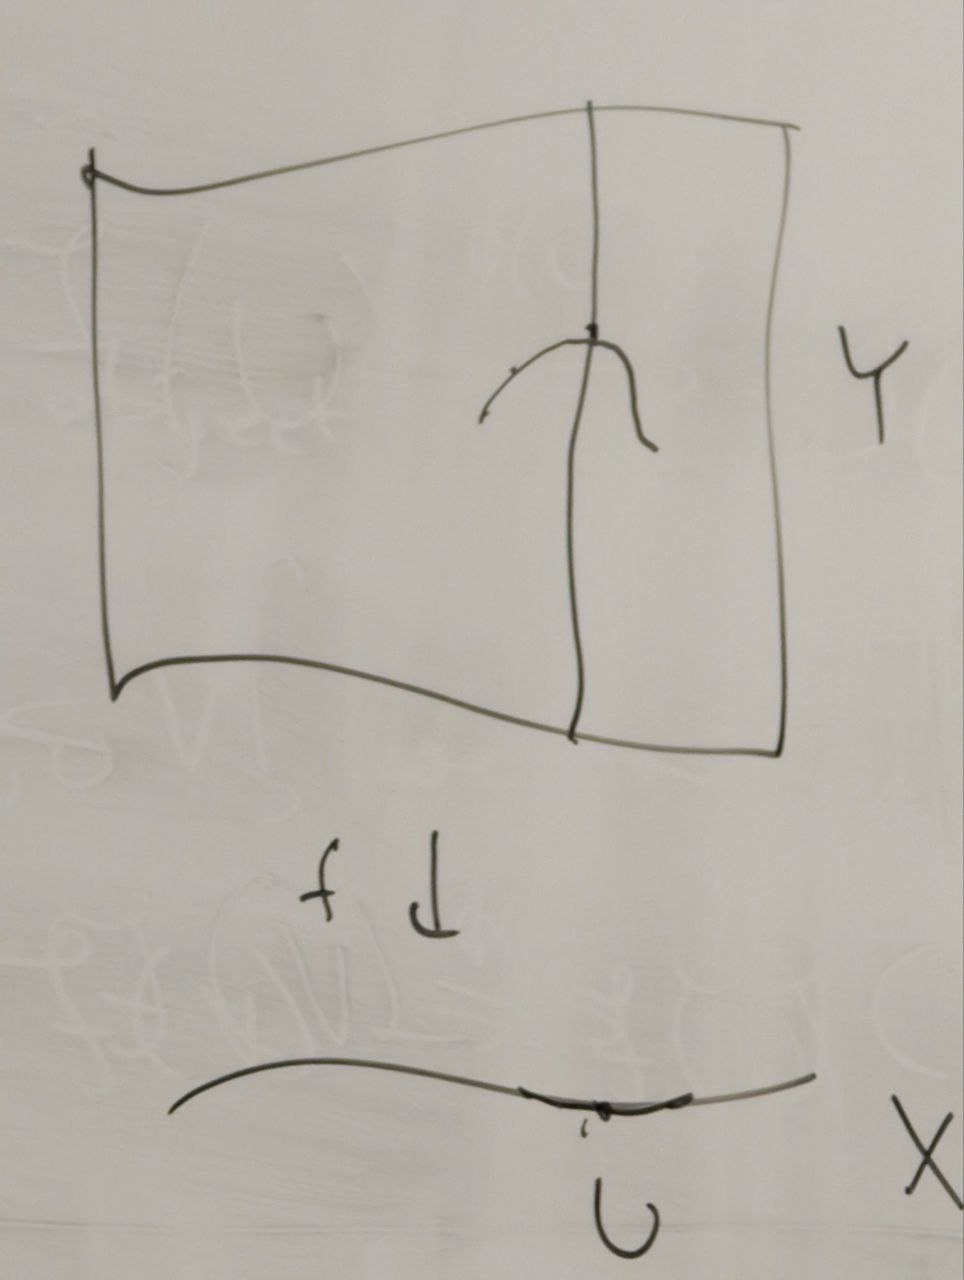
\includegraphics[width=0.4\textwidth]{img/section}
        \caption{}
    \end{figure}

    The \textit{stalk} of \(x\in X\) is \(\varinjlim_{U \ni x} \mathcal{F}(U)\).

    If \(\mathcal{F}\) is a presheaf of analytic functions on \(X = \mathbb{C}\), what is the stalk at \(x = 0\)?

    It is defined by the taylor series. So it contains power series with positive radius of convergence.

    Suppose \(U \subset X\) is open. Let \(U_\alpha\) be an open cover of \(U\). We also have \(\bigcup_{\alpha \in I} U_\alpha = U\).

    We have two obvious maps \(\prod_{\alpha \in I} \mathcal{F}(U)\) to \(\prod_{\beta ,\gamma \in I} \mathcal{F} (U_\beta \cap U_\gamma)\).

    \[
        \begin{tikzcd}
            \prod_{\alpha \in I} \mathcal{F}(U) \ar[r, bend left, "\phi : \alpha \mapsto \beta"] \ar[r, bend right, "\psi : \alpha \mapsto \gamma"] & \prod_{\beta, \gamma\in I} \mathcal{F}(U_\beta \cap U_\gamma)
        \end{tikzcd}
    \]

    Let's take a look into this. We have sections \((s_\alpha)_\{ \alpha \in I \} \mapsto (t_{\beta, \gamma})_{\beta, \gamma}\).

    \(\phi((s_\alpha))_{\beta,\gamma} = \operatorname{Res}_{U_\beta, U_\beta \cap U_\gamma} s_\beta \)
    
    \(\psi((s_\alpha))_{\beta ,\gamma} = \operatorname{Res}_{U_\gamma, U_\beta \cap U_\gamma} s_\gamma\).
    
    

    Thus we have:

    \[
        \begin{tikzcd}
            \mathcal{F}(U) \ar[r] & \prod_{\alpha \in I} \mathcal{F}(U) \ar[r, bend left, "\alpha \mapsto \beta"] \ar[r, bend right, "\alpha \mapsto \gamma"] & \prod_{\beta, \gamma\in I} \mathcal{F}(U_\beta \cap U_\gamma)
        \end{tikzcd}
    \]

    This diagram commutes.

    Let \(\mathcal{F}: \operatorname{Open}(X) \to \mathcal{C}\). If \(\Delta \in \operatorname{ob} \mathcal{C}\) then,

    \[
        \begin{tikzcd}
            \Delta \ar[d,dotted] \ar[rd] \\ \mathcal{F}(U) \ar[r] & \prod \mathcal{F}(U_\alpha) \ar[r, bend right] \ar[r, bend left] & \prod \mathcal{F} (U_\beta \cap U_\gamma)
        \end{tikzcd}
    \]

    If \(s_\alpha \in \mathcal{F}(U_\alpha)\) is a collection of sections so that \(\forall \beta ,\gamma\), \(s_\beta\) and \(s_\gamma\) agree on overlaps, i.e. \(\operatorname{Res}_{U_\beta, U_\beta \cap U_\gamma} s_\beta = \operatorname{Res}_{U_\gamma , U_\beta \cap U_\gamma} s_\gamma\) then \(\exists s\in \mathcal{F}(U)\) such that \(\operatorname{Res}_{U, U_\alpha} s = s_\alpha\) for all \(\alpha\).

    This is the sheaf axiom.

    Since there exists the empty product, we have to have a terminal object. But in our definition of the category of rings, we are excluding the zero ring so we don't have a final object in that category. But then we cannot define schemes. We need to modify some things.

    \subsection*{Presheaf which is not a Sheaf}

    We want to define sheaves. Consider the following example:

    Let \(X = \mathbb{R}\) and \(\mathcal{F} =\) sheaf of continuous functions \(X \to \mathbb{Z}\). Let \(\mathcal{G} =\) presheaf of constant \(\mathbb{Z}\)-valued functions on \(X\).

    Then, \(\mathcal{G}(U) = \mathbb{Z}\) for all \(U\neq \varnothing\).

    \(\mathcal{G}(\phi) = (0)\).

    \(\mathcal{F}\) agrees with \(\mathcal{G}\) on connected sets. But not necessarily on disconnected sets.

    \(\mathcal{G}\) is not a sheaf!

    What are the stalks of \(\mathcal{F}\) and \(\mathcal{G}\)?

    In both cases, the stalk at every point is \(\mathbb{Z}\).

    Furthermore, in the category of presheaves, there is a map \(\mathcal{G} \to \mathcal{F}\) in the sense that we have \(\mathcal{G}(U) \to \mathcal{F}(U)\) which is essentially the identity. On the stalks, this is an isomorphism.

    In general, if \(\mathcal{G}\) and \(\mathcal{F}\) are both presheaves on \(X\) and \(\phi: \mathcal{G} \to \mathcal{F}\) is a morphism of presheaves, then \(\forall x\in X\), \(\phi\) induces a map \(\phi_x\) sending stalks to stalks: \(\phi_x : \mathcal{G}_x \to \mathcal{F}_x\).

    \[
        \begin{tikzcd}
            \mathcal{F}(U) \ar[r] & \mathcal{F}(W) & \mathcal{F}(V) \ar[l] \\ \mathcal{G}(U) \ar[u] \ar[r] & \mathcal{G}(W) \ar[u] & \mathcal{G} (V) \ar[u] \ar[l]
        \end{tikzcd}
    \]

    is commutative.

    Note that, we can thus have two different presheaves with the same stalks. We don't want this, stalk should contain all the data of a sheaf.

    Slogan: A sheaf is a local object, i.e. determined by local data: stalks and \textit{compatibility of nearby stalks}.

    \section*{Wednesday, 9/10/2025}
    
    Let \(\mathcal{F}\) be a presheaf, \(U \subset X\) open. We can look at sections of \(X\) inside \(U\). Let \(\mathcal{F}_x\) be the stalk of \(\mathcal{F}\) at \(x\). We have:

    \[
        \mathcal{F}(U) \to \text{(compatible germs over \(U\))} \subset \prod_{x\in U} \mathcal{F}_x 
    \]

    \[
        s \mapsto (s_x)_{x\in U}
    \]

    Claim: if \(\mathcal{F}\) is a sheaf, this map is a bijection.

    Suppose sections \(s,t \in \mathcal{F}(U)\) and \(s_x = t_x\) for all \(x\in U\).

    Germs \(s_x\) and \(t_x\) are equal implies for all \(x\in X\) we can find an open set \(V_x \subset U\) containing \(x\) and a section \(r\in \mathcal{F}(V_x)\) such that \(s_x  = [(r,V_y)] = t_x\).
    
    Meaning, \(\operatorname{Res}_{U,V_x} s = r = \operatorname{Res}_{U, V_x} t\).

    Note that \(\bigcup_x V_x = U\). Sheaf axiom says that two sections on an open cover are the same. So, \(s=t\). This proves that the map is injective.

    Suppose we have \((s_x)_{x\in U}\) are compatible.

    For each \(x\), define \(V_x \ni x\) and \(\sigma_x \in \mathcal{F}(V_x)\), \(s_x = (\sigma_x)_x\). We want to glue together the \(\sigma_x\). We want the gluability part of the sheaf axiom.

    Claim: \(\forall x,y, \operatorname{Res}_{V_x, V_x \cap V_y} \sigma_x = \operatorname{Res}_{V_y, V_x \cap V_y} \sigma_y\).
    
    \(\forall x,y, \exists \sigma \in \mathcal{F}(U)\) such that \(\operatorname{Res}_{U,V_y} \sigma = \sigma_x \forall x\). So we're done. 

    \begin{definition}
        The \'etal\'e space \([\mathcal{F}]\) of a sheaf \(\mathcal{F}\) is the disjoint union of their stalks with the topology generated by

        \[
            \left\{ [(s,x)] \mid x\in U, s\in \mathcal{F}(U) \right\} 
        \]
    \end{definition}

    We then have a map \([\mathcal{F}] \to X\). Compatible germs map to open neighborhood.

    Now suppose we have \(X \xrightarrow{f} Y\). If \(\mathcal{F}\) is a sheaf we can define the \textit{pushforward of \(\mathcal{F}\) by \(f\)}.

    \[
        f_{\ast} (\mathcal{F})(U) = \mathcal{F}(f ^{-1} (U))
    \]

    Example: suppose \(X = \{ y \}\) and \(f\) is the inclusion map.

    Let \(c \in \operatorname{ob} \mathcal{C}\). Let \(\mathcal{F}_{y,c}=\) sheaf over \(y\) with value \(c\). \(f: \{ y \} \hookrightarrow y \in Y\).
    
    \[
        f_{\ast} \mathcal{F}_{y,c}(U) = \begin{dcases}
            c, &\text{ if } y\in U \\
            0, &\text{ if } y\notin U
        \end{dcases}
    \]

    \begin{definition}
        A \textit{ringed space} is a pair \((X, \mathcal{O}_X)\) where \(X\) is a topological space and \(\mathcal{O}_X\) is a sheaf of commutative rings on \(X\).
    \end{definition}

    Examples: 

    \begin{enumerate}[label=\arabic*)]
        \item \(X\) is a topological space, \(\mathcal{O}_X\) is the sheaf of continuous \(\mathbb{R}\)-valued functions.
        \item \(X\) is a smooth manifold, \(\mathcal{O}_X\) is the sheaf of smooth functions on \(X\).
        \item \(X\) is a Riemann surface, \(\mathcal{O}_X\) is the sheaf of analytic functions on \(X\).
    \end{enumerate}
    
    \begin{theorem}
        The category of presheaves of \(\begin{pmatrix}
            \text{abelian grps} \\
            \text{vector spaces} \\
            \text{etc}
        \end{pmatrix} \) forms an abelian categories.
    \end{theorem}

    To prove this, we need to be able to compute kernels, images, cokernels.

    Let \(\phi : \mathcal{F} \to \mathcal{G}\) be a morphism of presheaves. We \textit{do it by sections}:

    \((\ker \phi)(U) = \ker \mathcal{F}(U) \xrightarrow{\phi(U)} \mathcal{G}(U)\).

    \((\operatorname{im} \phi )(U) = \operatorname{im} \phi(U)\) 

    \((\operatorname{coker} \phi) (U) = \operatorname{coker} \phi(U)\)

    If \((X, \mathcal{O}_X)\) is a ringed space, we can define a presheaf \(\mathcal{F}\) of \(\mathcal{O}_X\)-modules to be a presheaf of abelian groups and structure of \(\mathcal{O}_X(U)\)-module on each \(\mathcal{F}(U)\) compatible with restriction maps.

    Example: Let \(E \to X\) be a vector bundle.

    Let \(\mathcal{O}_X\) be the sheaf of rings of continuous functions over \(X\) and \(\mathcal{F}\) be the sheaf of continuous sections of \(E \to X\).

    The category of sheaves is a full subcategory of the category of presheaves. This means, morphisms of sheaves are the same as morphism of presheaves which just happen to be sheaves.

    The category \(\operatorname{Ab}_X\) of sheaves of abelian groups is again an abelian category.

    \begin{lemma}
        If \(\phi : \mathcal{F} \to \mathcal{G}\) is a morphism of sheaves of abelian groups over \(X\), then the presheaf kernel of \(\mathcal{F} \to \mathcal{G}\) is a sheaf:

        \(\mathcal{H} (U) \coloneqq \ker \left(\mathcal{F}(U) \xrightarrow{\phi(U)} \mathcal{G}(U)\right)\) is a sheaf.
    \end{lemma}

    \begin{proof}
        Given an open cover \(U = \bigcup_{\alpha} U_\alpha\) and given \(h \in \mathcal{H} (U)\) such that \(\operatorname{Res}_{U,U_\alpha}(h) = 0\) for all \(\alpha\) we have \(h = 0\).

        Reason: \(\mathcal{H}(U) \subset \mathcal{F}(U)\) so we only need to check if \(h\) is \(0\) in \(\mathcal{F}(U)\) which follows from the sheaf axiom.

        Given \(h_\alpha \in \mathcal{H}(U_\alpha)\) such that \(\operatorname{Res}_{U_\alpha , U_\alpha \cap U_\beta} h_\alpha = \operatorname{Res}_{{U_\beta , U_\alpha \cap U_\beta}} h_\beta \forall \alpha ,\beta \) then \(\exists h \in \mathcal{H}(U) \in \ker \left( \mathcal{F}(U_\alpha) \xrightarrow{\phi(U_\alpha)} \mathcal{G}(U_\alpha) \right)\).

        \(\phi(U_\alpha \cap U_\beta) \left( \operatorname{Res}_{U_\alpha , U_\alpha \cap U_\beta} h_\alpha - \operatorname{Res}_{U_\beta , U_\alpha \cap U_\beta} h_\beta \right) = 0\) 

        We have \(\operatorname{Res}_{U_\alpha , U_\alpha \cap U_\beta} \phi(U_\alpha)(h_\alpha) = \operatorname{Res}_{U_\beta , U_\alpha \cap U_\beta} \phi(U_\beta) (h_\beta)\).

        \(h_\alpha \in \mathcal{F}(U_\alpha)\) which maps to \(0\) on \(\mathcal{G}(U_\alpha)\) 

        \(h_\beta \in \mathcal{F}(U_\beta)\) maps to \(0\) in \(\mathcal{G}(U_\beta)\).

        Then \(\operatorname{Res}_{U_\alpha , U_\alpha \cap U_\beta} h_\alpha = \operatorname{Res}_{U_\beta , U_\alpha \cap U_\beta} h_\beta\) 

        By gluability \(\exists h \in \mathcal{F}(U)\) such that \(\operatorname{Res}_{U,U_\alpha} h = h_\alpha\).

        Question: Does \(h\in \mathcal{H}\)? WTS: \(\phi(U)(h) = 0\).
        
        \(\operatorname{Res}_{U,U_\alpha} \phi(U) (h) = 0 \forall \alpha\).

    \end{proof}

    In general, gluability on \(\mathcal{F}\) and separability on \(\mathcal{G}\) implies gluability on \(\mathcal{H}\).

    \section*{Friday, 9/12/2025}
    
    If \(\mathcal{F}, \mathcal{G}\) are sheaves and \(\phi: \mathcal{F} \to \mathcal{G}\) is a morphism, then if we take image in the category of presheaves, then \(\operatorname{im} (\phi) (U) = \phi(U)(\mathcal{F}(U)) \subset \mathcal{G}(U)\).

    Then \(\operatorname{im} (\phi)\) is not a sheaf.

    For sheaves, we need a different notion of images!

    The separability axiom is fine: if \(f_1, f_2\in \operatorname{im} (\phi)(U)\) and \(U = \bigcup_\alpha U_\alpha\) and \(\forall \alpha : \operatorname{Res}_{U, U_\alpha}(f_1) = \operatorname{Res}_{U,U_\alpha}(f_2)\) then \(f_1 = f_2\).

    Problem is gluability.

    Suppose \(g_\alpha \in \operatorname{im} (\phi) (U_\alpha)\) and \(\forall \alpha ,\beta\) we have \(\operatorname{Res}_{U_\alpha, U_\alpha \cap U_\beta} g_\alpha  = \operatorname{Res}_{U_\beta, U_\alpha \cap U_\beta} g_\beta\).

    Can we find a \(g\in \operatorname{im} (\phi)(U)\) such that \(\operatorname{Res}_{U,U_\alpha} (g) = g_\alpha\)?

    Note that since \(g_\alpha \in \operatorname{im} (\phi)(U_\alpha)\), there exists \(f_\alpha\in \mathcal{F}(U_\alpha)\) such that \(\phi(U_\alpha) (f_\alpha) = g_\alpha\).

    We can do this gluing if \(\operatorname{Res}_{U_\alpha , U_\alpha \cap U_\beta} f_\alpha = \operatorname{Res}_{U_\beta , U_\alpha \cap U_\beta}\) for all \(\alpha , \beta\) by gluability of \(\mathcal{F}\). But we don't necessarily have that, we can only deduce that \(\operatorname{Res}_{U_\alpha , U_\alpha \cap U_\beta} f_\alpha - \operatorname{Res}_{U_\beta , U_\alpha \cap U_\beta} f_\beta\)  is in \(\ker \phi(U_\alpha \cap U_\beta)\).

    Thus, if we want an abelian category of sheaves, we want a different notion of image and cokernels.

    \begin{theorem}
        If \(\mathcal{F}, \mathcal{G}\) are sheaves and \(\phi : \mathcal{F} \to \mathcal{G}\) is a morphism of sheaves which is an isomorphism at the stalk level, then \(\phi\) is an isomorphism.

        Isomorphism at the stalk level: \(\phi: \mathcal{F} \to \mathcal{G}\) induces \(\phi_x: \mathcal{F}_x \to \mathcal{G}_x\) for each \(x\in X\). We want this to be an isomorphism.

        Slogan: A sheaf is determined by its stalks.
    \end{theorem}

    \begin{proof}

        Let \(U\) be any open subset of \(X\). We want \(\phi(U): \mathcal{F}(U) \to \mathcal{G}(U)\) to be an isomorphism.

        Suppose \(f_1, f_2\in \mathcal{F}(U)\) such that \(\phi(U)(f_1) = \phi(U)(f_2)\). Then \(\forall x\in U\), the germ of \(f_1\), which we write as \(f_{1,x}\) and the germ of \(f_2\), \(f_{2,x}\) map to the same germ, i.e. \(\phi(U)(f_1)_x = \phi(U)(f_2)_x\) in \(\mathcal{G}_x\). So, \(f_{1,x} = f_{2,x}\) for all \(x\in U\). Thus \(\exists U_x \subset U\) such that \(\operatorname{Res}_{U,U_x} f_1 = \operatorname{Res}_{U,U_x} f_2\).

        By separability, \(f_1 = f_2\).

        Now we prove gluability. Let \(g\in \mathcal{G}(U)\). \(\forall x\in U\) we have \(g_x = \phi_x(f_x)\) for some (unique) \(f_x \in \mathcal{F}_x\).

        Then \(\exists f_{U_x} \in \mathcal{F}(U_x)\) such that \(f_{U_x}\) represents \(f_x\) where \(U_x\) is a neighborhood of \(x\).

        Then \(\phi(U_x)(f_{U_x}) = g_{U_x}\) which has stalk \(g_x\). Then there exists \(U_x \supset V_x \ni x\) such that \(\phi(V_x)(\operatorname{Res}_{U_x, V_x}f_{U_x}) = \operatorname{Res}_{U,V_x}(g)\).
        
        Define \(f_{V_x}^{\prime} = \operatorname{Res}_{U_x, V_x} f_{U_x}\). Then, \(\phi(V_x)(f^{\prime} _{V_x}) = \operatorname{Res}_{U, V_x} (g)\).

        Claim: \(\{ f^{\prime}_{V_x} \}\) agree on overlaps.

        Proof: \(\forall x,y\in U\) we have \(\operatorname{Res}_{V_x, V_x\cap V_y} (f^{\prime} _{V_x}) = \operatorname{Res}_{V_y, V_x\cap V_y}(f^{\prime}_{V_y})\). This is true stalk by stalk and \(\mathcal{F}\) is a sheaf. By gluability we can find \(f^{\prime} \in \mathcal{F}(U)\) such that \(\operatorname{Res}_{U,V_x} f^{\prime} = f^{\prime} _{V_x}\) for all \(x\).

        Therefore, \(\phi(U)(f^{\prime})_x = g_x\) for all \(x\). \(\phi(U)(f^{\prime}) = g\).

    \end{proof}

    Given a presheaf \(\mathcal{F}\) there exists at most one sheaf \(\mathcal{G}\) and morphism \(\mathcal{F} \to \mathcal{G}\) which is an isomorphism of stalks at each \(x\). The process of finding such a \(\mathcal{G}\) is called \textit{sheafification}.

    \begin{definition}
        [Sheafification] Let \(\mathcal{F}\) be a presheaf. We define its sheafification \(\mathcal{F} ^{\operatorname{sh}}\) in the following way:

        The stalks \(\mathcal{F}_x^{\operatorname{sh}}\) are the same as \(\mathcal{F}_x\).

        Compatibility is the same.

        Let us be very specific about what sections are.

        \(\mathcal{F}^{\operatorname{sh}} = \text{functions } U \to \coprod_{x\in U} \mathcal{F}_x\) such that each \(x\in U\) maps to \(f_x\in \mathcal{F}_x\) such that \(f_x\) are compatible as usual. 
    \end{definition}

    We need to check if \(\mathcal{F}^{\operatorname{sh}}\) is actually a sheaf, and if there exists a map \(\mathcal{F} \to \mathcal{F}^{\operatorname{sh}}\) which is an isomorphism at the stalk level.

    WTS: \(f_\alpha \in \mathcal{F}^{\operatorname{sh}}(U_\alpha)\) and \(\forall \alpha ,\beta\) we have \(\operatorname{Res}_{U_\alpha , U_\alpha \cap U_\beta} (f_\alpha) = \operatorname{Res}_{U_\beta , U_\alpha \cap U_\beta}(f_\beta)\) then \(\exists ! f \in \mathcal{F}^{\operatorname{sh}}(U)\).

    \(f_\alpha\) gives us a function \(U_\alpha \to \coprod_{x\in U_\alpha} \mathcal{F}_x\).
    
    \(f_\beta\) gives us a function \(U_\beta \to \coprod_{x\in U_\beta} f_x\).

    \(\forall x\in U_\alpha \cap U_\beta\) we have \(f_{\alpha, x} = f_{\beta , x}\).

    Define \(f_x = f_{\alpha , x}\) for some \(\alpha\) with \(x\in U_\alpha\).

    Now we need the map \(\mathcal{F} \to \mathcal{F}^{\operatorname{sh}}\). Consider \(\mathcal{F}(U) \to \mathcal{F}^{\operatorname{sh}}\) given by \(f \mapsto (x \mapsto f_x)\).
    
    We trivially have \(\mathcal{F}_x^{\operatorname{sh}} = \mathcal{F}_x\): let \(s_x = [(s\in \mathcal{F}(U), x)]\). \(s\) defines compatible germs in a neighborhood of \(x\) therefore a section of \(\mathcal{F}_x^{\operatorname{sh}}\) in a neighborhood of \(x\).

    \subsection*{Exponential Sequence for analytic functions on \(X = \mathbb{C} \setminus \{ 0 \}\)}

    Let \(\mathcal{O} =\) analytic functions [as additive group]

    \(\mathcal{O} ^\times =\) non-vanishing analytic functions [as multiplicative group]

    Let \(\underline{\mathbb{Z}}\) be sheaf of locally constant \(\mathbb{Z}\)-valued functions.

    We have the following:

    \[
        \begin{tikzcd}
            0 \ar[r] & \underline{\mathbb{Z}} \ar[r] & \mathcal{O} \ar[rr, "f \mapsto \exp(2 \pi i f)"] & & \mathcal{O}^\times \ar[r,"?"] & 0
        \end{tikzcd}
    \]

    Question: is this sequence exact?

    We can't take log uniquely in \(\mathcal{O}^\times\) so not for presheaves. But we can take log locally, so on the stalk level we can take log and thus this is a short exact sequence for sheaves!

    Slogan: Exactness for presheaves is determined on the section level, exactness for sheaves is determined on the stalk level.

    Let \(\phi : \mathcal{F} \to \mathcal{G}\) be a morphism of sheaves in an abelian category.

    \(\operatorname{im} (\phi)_{\text{sheaves}} = (\operatorname{im}(\phi)_{\text{presheaves}})^{\operatorname{sh}}\)

    \(\operatorname{coker}(\phi)_{\text{sheaves}} = (\operatorname{coker}(\phi)_{\text{presheaves}})^{\operatorname{sh}}\) 
    
    \begin{theorem}
        If \(\mathcal{F}\) is a presheaf, \(\mathcal{F}^{\operatorname{sh}}\) is the universal sheaf admitting a map from \(\mathcal{F}\).
    \end{theorem}

    Thus, if \(\mathcal{F}\) is a presheaf and \(\mathcal{G}\) is a sheaf and we have \(\mathcal{F} \to \mathcal{G}\) we have a unique \(\mathcal{F}^{\operatorname{sh}} \to \mathcal{G}\).
    
    \[
        \begin{tikzcd}
            \mathcal{F} \ar[r] \ar[rd] & \mathcal{F}^{\operatorname{sh}} \ar[d, dotted] \\ & G
        \end{tikzcd}
    \]

    Sheafification is a functor. There is also a forgetful functor from sheaves to presheaves.

    Sheafification is the left adjoint of the forgetful functor.

    If \(\mathcal{F}\) is a presheaf and \(\mathcal{G}\) is a sheaf,

    \[
        \begin{tikzcd}
            \operatorname{Mor}_{\text{sheaves}} (\mathcal{F}^{\operatorname{sh}}, \mathcal{G}) \ar[r, "\cong"] & \operatorname{Mor}_{\text{presheaves}} (\mathcal{F} , \mathcal{G}) 
        \end{tikzcd}
    \]

    \section*{Monday, 9/15/2025}

    \subsection*{Sheaf w.r.t.\ a base}
    
    Let \(X\) be a topological space and \(B\) a base for the topology on \(X\).

    A presheaf on \(X\) w.r.t.\ \(B\) is a contravariant functor from \(B\) to \(\mathcal{C}\).

    A sheaf on \(X\) w.r.t.\ \(B\) is a presheaf \(\mathcal{F}\) such that any section \(f\in \mathcal{F} (U)\) is determined uniquely by compatible restrictions to \(U_\alpha\) where \(U_\alpha \in B\) and \(\bigcup_{\alpha} U_\alpha = U\).

    \[
        \begin{tikzcd}
            \mathcal{F}(U) \ar[r] & \prod_{\alpha} \mathcal{F}(U_\alpha) \ar[r, bend right] \ar[r, bend left] & \prod_{\alpha,\beta,\gamma, U_\alpha \subset U_\beta \cap U_\gamma} \mathcal{F}(U_\alpha) \\ C \ar[u, dotted] \ar[ur]
        \end{tikzcd}
    \]

    If \(\mathcal{F}\) is a sheaf on \(X\) and \(B\) is a base then by forgetting some data we get a sheaf on \(X\) w.r.t.\ \(B\). In fact every sheaf on \(X\) w.r.t.\ \(B\) comes from a sheaf \(\mathcal{F}\) on \(X\) which is unique up to unique isomorphism.

    Given \(\mathcal{F}_B\) a sheaf w.r.t.\ \(B\), \(B = \left\{ U_\alpha \mid \alpha \in I \right\} \) define:
    
    \[
        \mathcal{F} (U) \coloneqq \prod_{\alpha \mid U_\alpha \subset U} \mathcal{F}_B (U_\alpha) \rightrightarrows \prod_{\alpha ,\beta, \gamma \mid U_\alpha \subset U_\beta \cap U_\gamma} \mathcal{F}_B (U_\alpha)
    \]

    Now take stalks.

    Let \(\mathcal{F}_{B,x} = \varinjlim_{U\in B, x\in U} \mathcal{F} _B (U)\).

    A set of elements \(s_x\in \mathcal{F}_{B,x}\) where \(x\in U \in \operatorname{Open} (X)   \) is compatible if \(\forall x\in U \exists V\in B, x\in V\) and a section \(s_V \in \mathcal{F}_B (V)\) suh that \((s_V)_x = s_x \forall x\in V\).
    
    Let \(\mathcal{F}\) be the sheaf given by stalks \(\mathcal{F}_{B,x}\) and this is compatibility.

    \subsection*{Gluing Sheaves}

    Now, suppose \(X\) is a topological space and \(\mathcal{F}\) is a sheaf on \(X\) and also \(X\) has an open cover: \(X = U_1 \cup U_2\).

    Consider the restriction of \(\mathcal{F}\): \(\eval{\mathcal{F}}_{U_i}\) which iis the sheaf which we obtain from \(\mathcal{F}\) by restricting to open sets contained in \(U_1\).

    This means \(\eval{\mathcal{F}}_{U_1}\) is a contravariant functor from \(\operatorname{Open}(U_i)\) to \(\mathcal{C}\) such that:

    \(\forall U \subset U_i: \eval{\mathcal{F}}_{U_i}(U) = \mathcal{F}(U)\)

    \(\forall V \subset U \subset U_i: \operatorname{Res}_{U, V}\) on \(\eval{\mathcal{F}}_{U_i}\) is the same as on \(\mathcal{F}\).

    Which means, if we have a sheaf on \(U_1\cup U_2\), we can get sheaves on \(U_1\) and \(U_2\).

    Can we do the reverse? Given sheaves \(U_1\) and \(U_2\) can we get a sheaf on \(U = U_1\cup U_2\)?

    Consider sheaves \(\mathcal{F}_1\) on \(U_1\) and \(\mathcal{F}_2\) on \(U_2\).

    We want something akin to \(\eval{\mathcal{F}_1}_{U_1\cap U_2} \cong \eval{\mathcal{F}_2}_{U_1\cap U_2}\) but this is not enough data. We actually want the following:

    Suppose we have isomorphism \(i: \eval{\mathcal{F}_1}_{U_1 \cap U_2} \to \eval{\mathcal{F}_2}_{U_1\cap U_2}\) then there exists a unique sheaf on \(X\) such that \(\eval{\mathcal{F}}_{U_1} \cong \mathcal{F}_1\) and \(\eval{\mathcal{F}}_{U_2} \cong \mathcal{F}_2\).
    
    \(\forall \in U_i\) the stalk \(\mathcal{F}_x\) is in fact \((\mathcal{F}_i)_x\).

    For \(x\in U_1\cap U_2\): \(\mathcal{F}_x = (\mathcal{F}_{1,x} \coprod \mathcal{F}_{2,x}) / \sim_i\).

    Suppose \(X = \bigcup_{\alpha \in I} U_\alpha\) and \(\mathcal{F}_\alpha\) is a sheaf on \(U_\alpha\). For all \(\alpha , \beta : \eval{\mathcal{F}_\alpha}_{U_\alpha \cap U_\beta} \to \eval{\mathcal{F}_\beta}_{U_\beta \cap U_\alpha}\) is an isomorphism. Further, \(\forall \alpha ,\beta \gamma\) we have:

    \[
        \eval{i_{\beta, \gamma}}_{U_\alpha \cap U_\beta \cap U_\gamma} \circ \eval{i_{\alpha , \beta}}_{U_\alpha \cap U_\beta \cap U_\gamma} = \eval{i_{\alpha , \gamma}}_{U_\alpha \cap U_\beta \cap U_\gamma}
    \]

    [This is needed for \(\sim_i\) to be an equivalence relation].

    Then we can glue together to get a sheaf \(\mathcal{F}\) on \(X\).

    \subsection*{Pullback sheaves}

    Let \(\mathcal{F}\) be a sheaf on \(Y\) and \(X \xrightarrow{f} Y\).

    The \'etal\'e space of \(f^{-1} \mathcal{F}\) is the pullback of the \'etal\'e space of \(\mathcal{F}\) via \(X \xrightarrow{f} Y\).

    If we think about \(\mathcal{F}\) as an \'etal\'e space, then we have a map \(\mathcal{F} \to Y\), and we have \(X \to Y\). Then we have a fiber product:

    \[
        \begin{tikzcd}
            X \times_Y \mathcal{F} \ar[r] \ar[d] & \mathcal{F} \ar[d] \\ X \ar[r] & Y
        \end{tikzcd}
    \]

    Define presheaf \(\mathcal{G}\) by \(\mathcal{G}(U) = \varinjlim_{V \supset f(U)} \mathcal{F}(V)\)

    Then let \(f^{-1} (\mathcal{F}) = \mathcal{G}^{\operatorname{sh}}\).

    Example: Let \(y\in Y\) and let \(f: \{ y \} \to Y\) by \(f(y) = y\).

    Then \(f ^{-1} \mathcal{F}\) is a sheaf on \(\{ y \}\).
    
    \[
        \mathcal{G}(\{ y \}) = \varinjlim_{V\ni y} \mathcal{F} l(V) = \mathcal{F}_y
    \]

    Clean way of saying this: \(f ^{-1}\) is the left adjoint of \(f_{\ast}\).

    Meaning: suppose \(X \xrightarrow{f} Y\) with \(\mathcal{F}, \mathcal{G}\) sheaves on \(X,Y\) respectively. Then,

    \[
        \operatorname{Mor}_{\operatorname{Sh} (X)} ( f ^{-1} (\mathcal{G}), \mathcal{F}) \to \operatorname{Mor}_{\operatorname{Sh} (Y)} (\mathcal{G}, f_{\ast} \mathcal{F})
    \]

    \subsection*{Spectrum}

    Let \(A\) be a commutative ring. Then \(\operatorname{Spec} A\) is the set of prime ideals.

    A `function' \(f \in A\) `vanishes' at a point \(P \in A\) if \(f \in P\).

    Define \(V(f) = \{ P \in \operatorname{Spec} A \mid f\in P \}\).

    We want \(V(f)\) to be closed.

    Consider the topology on \(\operatorname{Spec} A\) defined by the subbase \(V(f) ^{c} \).

    For example, \(A = \mathbb{C} [x] \implies \operatorname{Spec} A = \{ (x-c) \} \cup \{ (0) \}\).

    Then closed sets are finite collections of complex numbers.

    So, open sets are \(\mathbb{C}\) and all but finitely many points but we aren't allowed to delete \((0)\).

    Note that this space isn't Hausdorff since \(\overline{(0)} = \mathbb{C}\).

    [insert picture, \(\mathbb{C}\) is a line and the point \((0)\) is smeared over the line]
    \begin{figure}[H]
        \centering
        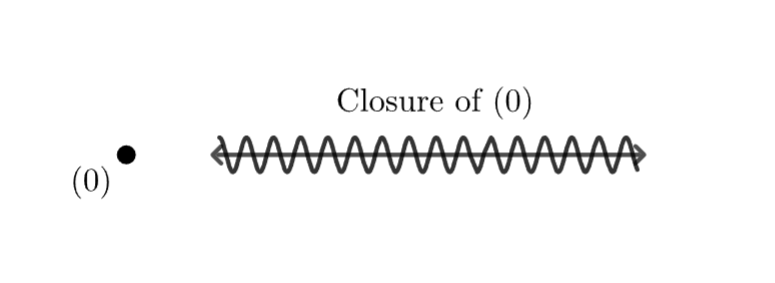
\includegraphics[width=0.8\textwidth]{img/SpecCx}
        \caption{$\operatorname{Spec}\mathbb{C}[x]$}
    \end{figure}

    \begin{remark}
        If \(I\) is any ideal we can define \(V(I) = \left\{ P \in \operatorname{Spec} A \mid I \subset P \right\} = \bigcap_{f\in I} V(f)\) is closed.
    \end{remark}

    \section*{Wednesday, 9/17/2025}
    
    We set up some definition:

    Let \(A\) be a ring, \(\operatorname{Spec} A\) the set of prime ideals. Let \(a\in A\) be a `function'.

    Define: \(V(a) = \left\{ P \in \operatorname{Spec} A \mid a\in P \right\}\).

    \(D(a) \coloneqq V(a) ^{c}\).

    Note that, \(V(ab) = \left\{ P \in \operatorname{Spec} A \mid ab\in P \right\} = V(a) \cup V(b)\).

    De Morgan \(\implies D(ab) = D(a) \cap D(b)\) so closed under intersection.

    Then the zariski topology is defined by the \textit{base} \(D(a)\).

    Suppose we have \(A \xrightarrow{\phi} B\). Then we have \(\operatorname{Spec} B \xrightarrow{f} \operatorname{Spec} B\) where \(f(P) = \phi ^{-1} (P)\).
    
    \begin{theorem}
        This function is continuous.
    \end{theorem}

    \begin{proof}
        WTS: \(f ^{-1} (\text{open})\) is open. Any open set can be written as \(\bigcup_{\alpha \in I} D(a_\alpha)\).

        \(f ^{-1} \left( \bigcup_\alpha D(a_\alpha) \right) = \bigcup_\alpha f ^{-1} (D(a_\alpha))\).

        Thus ETS: \(f ^{-1} (D_{\operatorname{Spec} A}(a_\alpha)) = D_{\operatorname{Spec} B}(f(a_\alpha))\).
        
        \(f(a_\alpha) \notin P \iff a_\alpha \notin \phi ^{-1} P \iff \phi(a_\alpha) \notin P\).
    \end{proof}

    Recall \(V(I) = \left\{ P\in \operatorname{Spec} A \mid I \subset P \right\}\). Abuse of notation: \(V((f)) = V(f)\). Then, \(V(I) = \bigcap_{f\in I} V(f)\) is closed. 

    \begin{proposition}
        There is a bijective correspondence between \(V(I)\) and \(\operatorname{Spec} A / I\).

        This correspondence is in fact bicontinuous if we endow \(V(I)\) with its subspace topology.
    \end{proposition}

    \begin{remark}
        A basis for \(V(I)\) is given by \(D(a) \cap V(I)\) which is the complement in \(V(I)\) of \(V(f) \cap V(I) = V((f) + I)\).

        If \(J \subset A / I\) is the ideal \(((f)+I) / I\) then \(V(J)\) corresponds to \(V(f) \cap V(I)\).
    \end{remark}

    To what extent do we have a bijective correspondense between ideals and closed subsets?

    If we have an ideal \(I\) we can go to a closed subset \(V(I)\).

    However, if we have a closed subset \(Z\) we can go to the set \(\left\{ f \in A \mid f\in P\, \forall P \in Z \right\}\).

    aka from \(Z\) we get the ideal of stuff that vanishes in \(Z\). This is not quite a bijective correspondense.

    Example: \((x)\) and \((x^2)\) both give us the same closed subset.

    We need to take the radical \(\operatorname{rad} (I)\) [other notation: \(\sqrt{I}\)].

    \(\operatorname{rad} (I) = \sqrt{I} = \bigcap_{P \in \operatorname{Spec} A, I \subset P} P\) 

    Suppose \(I = (x^2) \subset k[x]\). \((x^2) \subset P \iff (x) \subset P\).

    eg \(\operatorname{Spec} k[x] / (x^2)\) has picture of a point and a line.

    [insert picture]

    Let \(\mathbb{A}^1\) be an affine line: \(\operatorname{Spec} k[x]\).

    What does a map \(\mathbb{A}^1 \to \mathbb{A}^1\) look like?

    Let \(\mathbb{A}^1 \to \mathbb{A}^1\) be \(\operatorname{Spec} k[x] \to \operatorname{Spec} k[y]\).

    It corresponds to a ring homomorphism in the opposite direction: \(k[y] \to k[x]\).

    If we want to classify all such homomorphism, we should worry about what happens on the \(k\)-level. But when one is talking about varities, we are really talking about varities over a particular field, so we are essentially talking about a diagram like this:

    Note: Provisional definition of an affine variety: We can only talk about varities over a field \(k\). Consider \(\operatorname{Spec} A \to \operatorname{Spec} k\) where \(A\) is a finitely generated \(k\)-algebra. Then we have \(a_1, \cdots , a_n \in A\). We can look at \(\phi: k[x_1, \cdots , x_n] \to A\) which follows \(x_i \mapsto a_i\). Then \(A \cong k[x_1, \cdots , x_n] / I, \ker \phi = I\). 

    \[
        \begin{tikzcd}
            \mathbb{A}^1 \ar[rr] \ar[rd] & & \mathbb{A}^1 \ar[ld] \\ & \operatorname{Spec} k
        \end{tikzcd}
    \]

    So we are essentially talking about morphims of varities over \(\operatorname{Spec} k\). Then in the ring level we have: 

    \[
        \begin{tikzcd}
            k[x] & & k[y] \ar[ll] \\ & k \ar[ul] \ar[ur]
        \end{tikzcd}
    \]

    We only need to see where \(y\) goes. \(y\) maps to a polynomial \(p(x)\). So the morphisms are exactly what we want.

    Example: suppose \(k\) is algebraically closed and consider the map \(y \mapsto x^2\).

    What are the points on \(\operatorname{Spec} k[x]\)? Note that \(k[x]\) is a PID, so every ideal must be a scalar multiples of some polynomial \(f\). Since \(k\) is algebraically closed any polynomial \(f\) factors into linear factors. Thus, prime ideals are precisely \((x-a)\) [and \((0)\)].

    Thus, there is a bijective correspondence between \(\operatorname{Spec} k[x]\) and \(k \cup \{ \eta \}\) [\(\eta\) corresponds to the \((0)\) ideal. We call it the \textit{generic point}].
    
    Then, we have:

    \[
        \begin{tikzcd}
            & y \ar[r, mapsto] & x^2 \\
            & k[y] \ar[r] & k[x] \\
            (x-a) \ar[d] & \operatorname{Spec} k[x] \ar[r] \ar[d] & \operatorname{Spec} k[y] \ar[d] & (y - a^2) \ar[d] \\
            a\ar[u] & k \cup \{ \eta \} \ar[u] \ar[r, dotted] & k \cup \{ \eta \} \ar[u] & a^2 \ar[u]
        \end{tikzcd}
    \]

    \(\phi ^{-1} ((x-a)) = \left\{ P(y) \mid P(x^2) \in (x-a) \right\} = \left\{ P(y) \mid P(a^2) = 0 \right\} = (y-a^2)\).
    
    \(\phi ^{-1} (0): P(x^2) \equiv 0 \implies P(y) \equiv 0\) so \(\eta \leftrightarrow \eta\).

    Consider \(\operatorname{Spec} \mathbb{R} [x]\). Here \(\mathbb{R} [x]\) has prime ideals \((0)\) and \((f(x))\) where \(f\) is irreducible.

    eg \(x^2 + 1\) is irreducible in \(\mathbb{R} [x]\).

    Note that \(\mathbb{R} [x] / (x^2 + 1) \xrightarrow{\cong} \mathbb{C}\).

    The isomorphism map is as follows: \(f(x) \mapsto f(i)\). But it could be \(f(x) \mapsto f(-i)\).

    For a real polynomial, the condition of vanishing at \(i\) and \(-i\) are the same. This kind of maximal ideal doesn't correspond to an element in the field. In fact they don't even correspond to an element in a field extension. They correspond to a pair of elements in a field extension!

    There are thus two types of maximal ideal in \(\mathbb{R} [x]\):

    \begin{enumerate}[label=\arabic*)]
        \item \((x-a)\) where \(a\in \mathbb{R}\).
        \item \(((x-\alpha)(x-\overline{\alpha})), \{ \alpha , \overline{\alpha} \} \subset \mathbb{C} \setminus \mathbb{R}\) 
    \end{enumerate} 

    In addition there iis one prime ideal which is not maximal, \((0)\).

    What about fields where there are a lot of extension fields?

    What about \(\operatorname{Spec} A\) where \(A\) has a zero divisor?

    One way we can obtain a ring with a zero divisor is starting with a nice ring and modding out a product: \(k[x,y] / (f(x,y)g(x,y))\).
    
    Then \(V(fg) = V(f) \cup V(g)\).

    Consider zero sets of \(f(x,y)=0\) and \(g(x,y)=0\). Our space is the union of these sets, neither of which are the whole space. There is a point whose closure is the first component, a point whose closure is the second component, but no generic point!

    [insert picture]

    What if \(f=g\) in this case?

    Consider \(k[x,y] / (y-x)^2\). We have the same space as \(k[x,y] / (y-x)\), but we have an infinitesimal!
    
    [insert picture]

    What about \(\operatorname{Spec} \mathbb{Q} [x]\)? Too hard

    Now suppose \(k\) is algebraically closed. What about \(\operatorname{Spec} k[x,y] = \mathbb{A}^2_k\)?

    Our maximal ideals are \((x-a, y-b)\). This corresponds to the point \((a,b)\).

    We also have the middle case \((f(x,y))\) which are the intermediate ideals. If \(f(x,y) = y - x^2\) then it's closure consists of itself and all the points on the parabola. We can think about it as smeared over the whole parabola.

    We have the zero ideal \((0)\) which is the minimal ideal. It corresponds to a generic point.

    There are \(3\) levels, so the space should be roughly \(3\) dimensional. This is the idea behind Krull dimension.

    \section*{Friday, 9/19/2025}
    
    Some more commutative algebra, and topology on Spec.

    \begin{theorem}
        \(\operatorname{Spec} A\) is quasi-compact. 
    \end{theorem}

    \begin{proof}
        Note: we basically want to show every open cover has a finite subcover. We use the word `quasi' because \(\operatorname{Spec} A\) is not Hausdorff.

        Let \(\bigcup_{\alpha \in I} U_\alpha = \operatorname{Spec} A\).
        
        Each \(U_\alpha\) has an open cover \(U_\alpha = \bigcup_{\beta \in J_\alpha}^{} D(f_{\alpha , \beta})\).

        Then, \(\operatorname{Spec} A = \bigcup_{\alpha \in I}^{} \bigcup_{\beta \in J_\alpha}^{} D(f_{\alpha , \beta})\).

        We can reduce in this way to covers by \(D(f_{\alpha , \beta})\) `affine opens'. Changing notation, we write \(\operatorname{Spec} A = \bigcup_{\alpha \in I}^{} D(f_\alpha)\).

        Consider the ideal \(J = (f_\alpha)_{\alpha \in I}\).

        Case 1: \(J \neq A\). Then there exists a maximal ideal \(\mathfrak{m} \supset J \ni f_\alpha\).

        \(\mathfrak{m} \leftrightarrow x \in \operatorname{Spec} A\) then \(x\in V(f_\alpha)\) and \(x\notin D(f_\alpha) \forall \alpha\). So \(x\notin \bigcup_{\alpha \in I}^{} D(f_\alpha) = \operatorname{Spec} A\) which is a contradiction.

        Case 2: \(J = A\). Then \(1 \in J\) so \(\exists g_\alpha\) and finite \(I_0 \subset I\) and \(g_\alpha\) such that \(\sum_{\alpha \in I_0} f_\alpha g_\alpha = 1\).

        Claim: \(\bigcup_{\alpha \in I_0}^{} D(f_\alpha) = \operatorname{Spec} A\).

        Claim \(\iff \forall x\in \operatorname{Spec} A \exists \alpha \in I_0\) such that \(x\in D(f_\alpha) \iff \forall P\) prime ideal \(\exists \alpha \in I_0\) such that \(f_\alpha \notin P\). This is true since otherwise \(1 = \sum_{\alpha \in I_0} f_\alpha g_\alpha \in P\) which is impossible.  
    \end{proof}

    At first glance the previous theorem seems unprovable without the noetherian condition. But we don't need it.

    \begin{definition}
        A topological space \(X\) is \textit{Noetherian} if every decreasing chain of closed subsets \(X = X_0 \supset X_1 \supset  X_2 \supset \cdots\) eventually stabilizes.
    \end{definition}

    We then have the following theorem:

    \begin{theorem}
        If \(A\) is a noetherian ring then \(\operatorname{Spec} A\) is a noetherian topological space.
    \end{theorem}

    \begin{proof}
        \(\exists\) bijective correspondence between closed subsets and radical ideals, i.e. ideals \(I = \sqrt{I}\). 

        \[
            X \to I(X) = \left\{ f\in A \mid f\in P \forall P \in X \right\}
        \]

        A decreasing chain of \(X_i\) gives an increasing chain of \(I(X_i)\) which stabilizes.
    \end{proof}

    This gives us: any field \(k\) is noetherian since the only ideal is \((0)\).

    \begin{theorem}
        [Hilbert] If \(A\) is Noetherian then \(A[x]\) is Noetherian.
    \end{theorem}

    Corollary: \(k[x_1, \cdots , x_n]\) is Noetherian.

    Corollary: \(\mathbb{A}^n_k = \operatorname{Spec} k[x_1, \cdots , x_n]\) is Noetherian.

    Corollary: A closed subspace of a Noetherian space is Noetherian. On the ring side, a quotient ring of a Noetherian ring is Noetherian.

    \subsection*{Connectedness}

    If \(X = U_1 \sqcup U_2\) which are open then it is disconnected. \(U_1\) and \(U_2\) will also be closed.

    Question: is \(\operatorname{Spec} k[x_1, \cdots , x_n]\) connected?

    Is \(\operatorname{Spec} k[x_1, \cdots , x_n] / I\) connected?
    
    \begin{theorem}
        The following conditions are equivalent:

        \begin{enumerate}[label=\arabic*)]
            \item \(\operatorname{Spec} A\) is disconnected.
            \item \(A \cong A_1 \times A_2\) for some \(A_1 \times A_2\) [here not considering the zero ring as a ring helps us]
            \item \(A\) has a non-trivial idempotent \(e\) [i.e. \(e\neq 0,1, e^2 = e\). If your space has two components you can think of a function that is \(1\) on one component and \(0\) on the other component, then that function must be an idempotent].
        \end{enumerate} 
    \end{theorem}

    \begin{proof}
        \(2 \implies 3:\) Let \(e = (1,0)\).
        
        \(3 \implies 2:\) Let \(A_1 = A e, A_2 = A(1-e)\). Then \(A_1 \times A_2 \xrightarrow{\cong} A\) by \((xe, y(1-e)) \mapsto xe + y(1-e)\).
        
        \(1 \implies 3:\) Suppose \(\operatorname{Spec} A = V(I) \sqcup V(J)\). Then \(I + J = A\) otherwise \(I + J \subset \mathfrak{m}\) and the corresponding point \(x \in \operatorname{Spec} A \in V(I) \cap V(J)\).

        Claim: \(\phi : A \to A / I \times A / J\) is surjective and its kernel is nilpotent.

        Surjectivity: we can find \(a\in A\) such that \(a \equiv 1 \mod I, a \equiv 0 \mod J\) since \(I + J = A\).

        Now, suppose \(x\in \ker \phi\). Then \(x\in I \cap J\).

        Recall that for every prime ideal \(P\) of \(A\) we have \(I \subset P\) or \(J \subset P\) thus \(I \cap J \subset P\).

        Thus \(I \cap J \subset \bigcap_{P \in \operatorname{Spec} A} P = \operatorname{rad} (0) = \operatorname{rad} A\).
        
        So, \(x\in \operatorname{rad} A\) is nilpotent.

        Let \(e\in A\) satisfy \(\phi(e) = (1,0)\). THen \(e^2 - e \in \ker \phi \implies e^2 - e\) is nilpotent.

        Suppose \((e^2 - e)^n \equiv  0\).

        Claim: \(E = 1-(1-e^n)^n\) is an idempotent.

        Proof: \(E^2 - E = E(1-E) = (1-e^n)^n(1-(1-e^n)^n)\) which is a multiple of \(e^n(1-e)^n\) so it is \(0\).
        
        \(E \in (e^n)\) and \((1-E) \in ((1-e)^n)\).

        \(2 \implies 1\): Suppose \(A = A_1 \times A_2\). Every prime ideal either contains \(((1,0)) = A_1 \times (0)\) or \(((0,1)) = 0 \times A_2\).

        Equivalently project \(P \subset A\) onto \(A_1\) and project it into \(A_2\). Exactly one of these projections is surjective: if \(\operatorname{proj}_{A_1} P = I_1 \subsetneq A_1\) and \(\operatorname{proj}_{A_2} P = I_2  \subsetneq A_2\), we have \((x,1)(1,y) = (x,y) \in P\) but individually not in \(P\) which is a contradiction.
    \end{proof}

    \begin{theorem}
        A topological space \(X\) is reducible if \(X = X_1 \cup X_2\) where \(X_1, X_2 \subsetneq X\) and \(X_1\) and \(X_2\) are closed.

        Every disconnected space is reducible.
    \end{theorem}

    The key theorem for tomorrow:

    \begin{theorem}
        TFAE:

        \begin{enumerate}[label=\arabic*)]
            \item \(\operatorname{Spec} A\) is irreducible.
            \item \(\operatorname{Spec} A\) has a generic point: \(\eta \in \operatorname{Spec} A\) such that \(\overline{\{ \eta \} } = \operatorname{Spec} A\)
            \item \(A\) has a minimum prime ideal: a prime ideal contained in all other prime ideals.
            \item \(\operatorname{rad} A\) is a prime ideal. 
        \end{enumerate} 
    \end{theorem}

    \section*{Monday, 9/22/2025}
    
    We can instead prove the following theorem:

    \begin{theorem}
        TFAE:

        \begin{enumerate}[label=\arabic*)]
            \item \(\operatorname{Spec} A\) is reducible.
            \item \(\operatorname{Spec} A\) has no generic point
            \item \(A\) has no minimal prime ideal.
            \item \(\operatorname{rad} A\) is not prime.
        \end{enumerate} 
    \end{theorem}

    \begin{proof}
        We prove \(1 \implies 2 \implies 3 \implies 4 \implies 1\).

        \(1 \implies 2\): Suppose \(\operatorname{Spec} A = X \cup Y\) where \(X,Y\) are closed and \(X,Y \subsetneq \operatorname{Spec} A\).

        If \(\eta \in \operatorname{Spec} A\) then either \(\eta \in X\) or \(\eta \in Y\).

        So, \(\overline{\{ \eta \}} \subset X\) or \(\overline{\{ \eta \} } \subset Y\) so no generic point.
        
        \(2 \implies 3\): If \(P\) and \(Q\) are prime ideals, then \(Q \in \overline{\{ P \}} \implies Q \in V(P) \implies P \subset Q\). If there is no generic point, then there is no prime ideal that is contained in all other prime ideals.
        
        \(3 \implies 4\): Since every prime ideal contains \(\bigcap_{P\in \operatorname{Spec} A} P = \operatorname{rad} A\) it follows that \(\operatorname{rad} A\) is not prime.

        \(4 \implies 1\): Since \(\operatorname{rad} A\) is not prime, we have \(f,g\in A\) such that \(fg\in \operatorname{rad} A\) but \(f,g\notin \operatorname{rad} A\). Thus, there exists \(P\in \operatorname{Spec} A\) so that \(f\notin P\) i.e. \(P \notin V(f)\) and \(g\notin \operatorname{rad} A\) i.e. \(Q \notin V(g)\). But \(fg\in \operatorname{rad} A\) implies all prime ideals lie in \(V(fg)\).

        Thus, \(V(f) \cup V(g) = \operatorname{Spec} A\).
    \end{proof}

    \begin{corollary}
        \(A\) is intrgral domain \(\iff \operatorname{Spec} A\) is irreducible and \(A\) has no non-zero nilpotents.
    \end{corollary}

    \begin{proof}
        \(A\) integral implies [\(fg\in (0) \implies f\in (0)\) or \(g\in (0)] \implies (0)\) is prime \(\implies (0)\) is the minimum prime ideal \(\implies \operatorname{Spec} A\) is irreudible. Further, if \(f^n = 0\) then \(f=0\) so no non-zero nilpotents.

        Other direction: if \(\operatorname{Spec} A\) is irreducible then \(\operatorname{rad} A\) is prime. If \(\operatorname{Spec} A\) has no non-zero nilpotents, then \(\operatorname{rad} A = (0)\). Thus \((0)\) is prime. Thus, \(fg = 0 \implies fg\in (0) \implies f \in (0)\) or \(g\in (0) \implies f=0\) or \(g=0\). Thus \(A\) is an integral domain.
    \end{proof}

    \begin{lemma}
        If \(A\) is an integral domain then any polynomial ring \(A[x_1, \cdots , x_n]\) is also an integral domain.
    \end{lemma}

    \begin{proof}
        Use induction on \(n\). ETS: \(A\) integral \(\implies A[x]\) integral.

        Suppose \(P(x) = \sum_{i=0}^n a_i x^i, Q(x) = \sum_{j=0}^m b_j x^j\) are non-zero of degree \(n\) and \(m\) respectively. We may assume that \(a_n \neq 0, b_m\neq 0\). Then \(P(x) Q(x) = \sum_{k=1}^{n+m} \sum_{i+j=k} a_i b_j x^k \). So, the \(x^{n+m}\) coefficient of \(P(x)Q(x)\) is \(a_n b_m \neq 0\). Thus, \(P(x)Q(x) \neq 0\). 
    \end{proof}

    Thus, polynomial rings over an integral domain are integral. In particular, polynomial rings over fields are integral.

    \begin{corollary}
        \(\operatorname{Spec} k[x_1, \cdots , x_n]\) is irreudiclbe when \(k\) is a field.
    \end{corollary}

    Note that \(\operatorname{Spec} k[x_1, \cdots , x_n]\) is the affine \(n\)-space over \(k\).

    A consequence of irreducibility: In an irreudcible topological space \(X\), the closure of a non-empty open set \(U\) is everything: \(\overline{U} = X\).

    Why? Note that \(U^c \cup \overline{U} \supset U^c \cup U = X\). 

    \begin{theorem}
        Every \(n \times n\) matrix over \(\mathbb{C}\) satisfies its own characteristic polynomial.
    \end{theorem}

    \begin{proof}
        Let \(M \in M_n(\mathbb{C})\). Let \(p_M\) be the characteristic polynomial. If \(\operatorname{disc} p_M(x) \neq 0\) then \(M\) is diagonalizable with distinct entries. Thus \(M \sim \begin{bmatrix}
            \lambda_1 & \cdots & 0 \\
            \vdots & \ddots & \vdots \\
            0 & \cdots & \lambda_n \\
        \end{bmatrix} \) where \(\lambda_i \neq \lambda_j\).

        Then \(p_M(x) = p_D(x) = (x-\lambda_1) \cdots (x-\lambda_n)\) and \(p_M(M) = p_D(D) = 0\).
        
        i.e. Cayley Hamilton theorem is trivial when eigenvalues are distinct.

        Now we can easily finish with algebraic geometry:

        \(\operatorname{disc} p_M(x) \neq 0\) is a non-empty open condition on \(\mathbb{A}^{n^2}_{\mathbb{C}}\). 

        Any identity that holds on a dense subset of \(\mathbb{A}^{n^2}_{\mathbb{C}}\) holds on \(\mathbb{A}^{n^2}_{\mathbb{C}}\). So we're done! 
    \end{proof}

    What is happening under the hood? Note that \(\operatorname{disc} p_M \cdot p_M(M)\) on \(M_n(\mathbb{C})\) is always zero, so it is in fact the zero polynomial.

    \begin{definition}
        A ring \(A\) is a Jacobson ring if the intersection of its maximal ideals is \((0)\).
    \end{definition}

    This is a stronger condition than being an integral domain: eg a valuation ring has only one max ideal and thus it is a Jacobson ring.

    \begin{theorem}
        Every polynomial ring over a field is a Jacobson ring.
    \end{theorem}

    \section*{Chapter 4: Define \(\mathcal{O}_{\operatorname{Spec} A}\)}

    \(\operatorname{Spec} \mathcal{O}_{\operatorname{Spec} A}\): sheaf of regular functions on \(\operatorname{Spec} A\).

    \(U \subset \operatorname{Spec} A\) is any open set. We want \(\mathcal{O}_{\operatorname{Spec} A}(U)\).

    Suppose \(A\) is an integral domain with fraction field \(K\).

    Then \(\mathcal{O}_{\operatorname{Spec} A}(U) \subset K\). Which elements of \(K\) count as regular on \(U\)?

    Suppose we have \(\frac{a}{b}\in K\). As long as \(b\) doesn't vanish on \(U\), we can talk about \(\frac{1}{b}\) on \(U\). Thus we can talk about \(\frac{a}{b}\) on \(U\).

    Recall if \(P\in \operatorname{Spec} A\) then we can take \(\mathbb{K} (P) = \operatorname{Frac}(A / P)\). For \(f\in A\) then \(f(P) \in \mathbb{K}(P)\) namely, \((f \mod P) \in A / P \subset \operatorname{Frac} (A / P)\).
    
    Thus \(a,b\in A, \frac{a}{b}\in \mathbb{K} (P)\) is problematic when \(b\in P\).
    
    We want to work more generally than integral domains. We want to use the sheaf machinery.

    Stalk POV:

    What is the \textit{set of germs of regular functions at} \(P\)?

    We're basicallly looking at fractions where the denominator doesn't belong to \(P\).

    Recall we have localization: \(A_P = \left\{ \frac{a}{b} \mid b \in A \setminus P \right\} / \sim\).

    Let \(A_P\) be the stalks and compatibility of a family of a map \(U \to \sqcup_{P\in U} A_P\) by \(P \mapsto s_P\) are compatible if \(\forall P\in U \exists V \subset U\) open neighborhood of \(P\) and a fraction \(\frac{a}{b}\) where \(b\) does not lie in any prime ideal in \(V\) such that \(\frac{a}{b}\) gives \(s_P\) for all \(P\in V\).

    Base POV:

    \(D(f) = \operatorname{Spec} A \setminus V(f)\) gives a base for the topology of \(\operatorname{Spec} A\).

    \(\mathcal{O}_{\operatorname{Spec} A}(D(f)) = A \left[ \frac{1}{f} \right] = A_f = S ^{-1} A \) where \(S = \{ 1, f, f^2, \cdots \}\). We don't want \(f\) to be nilpotent. This is just \(A[x] / (fx - 1)\).


    \section*{Wednesday, 9/24/2025}
    

    We need to check if \(\mathcal{O}_{\operatorname{Spec} A}(D(f)) \coloneqq A \left[ \frac{1}{f} \right]\) is well defined and satisfies the sheaf axioms.
    
    Well defined:

    \begin{proposition}
        \(D(f) = D(g) \implies A \left[ \frac{1}{f} \right] \cong A \left[ \frac{1}{g} \right]\).
    \end{proposition}

    \begin{proof}
        It suffices to show that \(f\) is invertible in \(A[1 / g]\) and \(g \) is invertible in \(A[1 / f]\).

        Thus it suffices to show that \(f\) is invertible in \(A[1 / g]\).

        Note that \(D(f) = D(g) \implies D(f) \subset D(g)  \implies V(g) \subset V(f) \implies f\) vanishes on every point of \(V(g)\), i.e. \(\forall P \in V(g), f\in P\).

        Thus, \(f\in \bigcap_{P\in V(g)} P = \operatorname{rad} (g)\).

        Thus, \(f^n \in (g)\), i.e. \(\exists a\in A\) such that \(f^n = ag \implies \frac{1}{g} = \frac{a}{f^n} \in A[1 / f]\). Thus \(g\in A[1 / f]\). QED.  
    \end{proof}

    Thus, \(\mathcal{O}_X(D(f))\) is well defined. 
    
    \begin{proposition}
        Suppose \(D(f) = \bigcup_{\alpha \in I} D(f_\alpha)\). WTS: \(\mathcal{O}_X(D(f))\) is the \textit{equalizer} of the following diagram:

        \[
            \begin{tikzcd}
                \prod_{\alpha \in I} \mathcal{O}_X (D(f_\alpha)) \ar[r, bend right,"\phi"] \ar[r, bend left,"\psi"] & \prod_{\alpha,\beta \in I} \mathcal{O}_X(D(f_\alpha)\cap D(f_\beta))
            \end{tikzcd}
        \]

        i.e. \(\mathcal{O}_X(D(f)) = \left\{ g \in \prod_{\alpha \in I} \mathcal{O}_X(D(f_\alpha)) \mid \phi(g) = \psi(g)  \right\} \) 
    \end{proposition}

    \begin{proof}

        Specializations:

        \begin{enumerate}[label=\arabic*)]
            \item \(D(f) = X\)
            \item \(I\) is finite. 
        \end{enumerate} 

        Note \(D(f) = \operatorname{Spec} A \left[ \frac{1}{f} \right] \) and \(A \left[ \frac{1}{f_\alpha} \right] = A \left[ \frac{1}{f} \right] \left[ \frac{1}{f_\alpha} \right] \). So WLOG we can assume that \(D(f) = X\). Then,

        \[
            \begin{tikzcd}
                A \ar[r] & \operatorname{Eq} \bigg(  \prod A \left[ \frac{1}{f_i} \right] \ar[r, bend left] \ar[r, bend right] & \prod A \left[ \frac{1}{f_i f_j} \right] \bigg)
            \end{tikzcd}
        \]

        \[
            \begin{tikzcd}
                a \ar[r] & \left( \frac{a}{1} \right) \ar[r, bend right] \ar[r, bend left] & \left( \frac{a}{1} \right) 
            \end{tikzcd}
        \]

        We prove injectivity first.

        Suppose \(a\in A\) is in the kernel. Then \(a\in A\) maps to \(0\) in each \(A[1 / f_i]\). Thus, \(a / 1 = 0\) in \(A[1 / f_i]\) for all \(i \in I\). Thus, for all \(i\in I\), \(a f_i^{k_i} = 0\) for some \(k_i \in \mathbb{N}\).
        
        Furthermore, \(\operatorname{Spec} A = \bigcup_{i\in I} D(f_i)\), \(\forall P\in \operatorname{Spec} A, \exists f_i\) such that \(f_i \notin P\).

        Thus, \((f_1, f_2, \cdots) = 1\).

        Thus \(\sum_{i} a_i f_i = 1\) for some finite collection of the \(f_i\).

        For every \(k\) we have \((f_1^k, f_2^k, \cdots ) = 1\).

        Thus, \(\sum_{i} a_{i,k} f_i^k = 1\) for some finite collection of \(i\). Choosing \(k \geq k_i\) for the finite collection of \(i\), we see that \((f_1^{k_1}, f_2^{k_2}, \cdots ) = 1\). So, \(\sum_{i} b_i f_i^{k_i} = 1 \implies \sum_{i} a b_i f_i^{k_i} = a  = 0\).

        Now suppose \(I\) is finite. we now want to show surjectivity.

        Suppose \(\forall i,j\) we have \(\frac{a_i}{f_i} = \frac{a_j}{f_j}\) in \(A \left[ \frac{1}{f_i f_j} \right] \).

        Then we can find \(k_{i,j}\in\mathbb{N}\) such that \((a_i f_j - a_j f_i) (f_i f_j)^{k_{i,j}} = 0\).
        
        Suppose \(a_i f_j = a_j f_i\) [special case]. Note that \((f_1, f_2, \cdots , f_n) = 1 \implies b_1 f_1 + \cdots +b_n f_n = 1\).

        Let \(a = a_1 b_1 + \cdots + a_n b_n\). Claim: \(a = \frac{a_i}{f_i}\) for all \(i\).

        WTS: \(a = \frac{a_1}{f_1} \iff f_1 a = a_1\). Recall \(f_1 a = f_1 a_1 b_1 + f_1 a_2 b_2 + \cdots + f_1 a_n b_n = f_1 a_1 b_1 + f_2 a_1 b_2 + \cdots + f_n a_1 b_n = a_1(b_1 f_1 + \cdots + b_n f_n) = a_1\) So we're done.
        
        What if \(a_i f_j = a_j f_i\) doesn't hold? Note that \(\frac{a_1}{f_1}= \frac{a_1 f_1}{f_1^2} = \frac{a_1 f_1^2}{f_1^3} = \cdots\). These power gives us bigger powers of \((f_i f_j)^{k_{i,j}}\). So we have proved for finite \(I\).
        
        Now suppose \(I\) is infinite.

        Let \(J\) be the finite subset such that \(\bigcup_{j\in J} D(f_j) = \operatorname{Spec} A\).

        Given compatible fractions \(\frac{a_j}{f_j}, \exists a\in A\) which is equal to all of them. Moreover \(a\) is unique: \(a = \frac{a_i}{f_i}\) for all \(i\in I\). 

    \end{proof}

    Some clarification about partition of unity.

    Let \(X = \bigcup_i U_i\) and \(\phi_i: U_i \to \mathbb{R}\), \(\phi_i(x)=\phi_j(x)\) in \(U_i \cap U_j\). A partition of unity of \(X\): we define on the cover \(U_i\) a collection of functions \(\psi_i: X \to \mathbb{R}\) sucht hat each \(\psi_i\) is \(0\) outside \(U_i\) and \(\sum_{i} \psi_i = 1\).

    Note that \(\sum_{i} \phi_i \psi_i = f: X \to \mathbb{R}\) with the property if \(x\in U_i, f(x) = \phi_i(x)\).

    In the proof, role of \(\psi\) is played by \(b_i f_i\) which vanishes on \(V(f_i)\) and thus is suppported on \(D(f_i)\).

    Therefore, the sheaf \(\mathcal{O}_X\) exists and satisfies \(\mathcal{O}_X(D(f)) = A \left[ \frac{1}{f} \right]\).

    What about open sets not of the form \(D(f)\)? Suppose \(X = \mathbb{A}^2_{\mathbb{C}} = \operatorname{Spec} \mathbb{C} [x,y]\). Define \(U = X - \{ (0,0) \}\).

    We can take a cover of \(U\) by \(D(f)\)s.
    
    Let \(U_1 = \operatorname{Spec} \mathbb{C} [x,y]\left[ \frac{1}{y} \right] \) and \(U_2 = \operatorname{Spec} \mathbb{C}[x,y]\left[ \frac{1}{x} \right]\). Then \(U = U_1 \cup U_2\).
    
    We have \(\mathbb{C} \left[ x, y, \frac{1}{x} \right] \times \mathbb{C} \left[ x,y,\frac{1}{y} \right] \to \mathbb{C}\left[ x,y,\frac{1}{xy} \right]\).
    
    Let \(f = \sum_{i,j} a_{ij} x^i y^j \in \mathbb{C} \left[ x,y,\frac{1}{x} \right]  \) and \(g = \sum_{i,j} b_{ij} x^i y^j \in \mathbb{C} \left[ x,y,\frac{1}{y} \right]\). Then \(a_{ij} = b_{ij}\), no negatives, some positives. Thus we have no extra functions.

    \section*{Friday, 9/26/2025}
    
    Recall:

    We constructed \(\mathcal{O}_X\) for \(X = \operatorname{Spec} A\) using the base \(D(f)\) the so called distinguished opens.

    \(\mathcal{O}_X(D(f)) = A[f ^{-1}]\).
    
    What is the stalk at \(x\in X \leftrightarrow P \subset A\)? We take a direct limit over all the open neighborhoods of \(x\), aka the sections.

    \(\mathcal{O}_{X,x} = \varinjlim_{D(f) \ni x} \mathcal{O}_X(D(f)) = \varinjlim_{f \notin P} A \left[ \frac{1}{f} \right]\).

    \(= \varinjlim_{f \in A \setminus P} A \left[ \frac{1}{f} \right] = (A \setminus P) ^{-1} A = A_P\).

    We have the same construction for \(A\)-modules. Let \(M\) be an \(A\)-module. We can construct a sheaf of \(\mathcal{O}_X\)-modules \(\widetilde{M}\) in exactly the same way:

    Define \(\widetilde{M}(D(f)) = M \left[ \frac{1}{f} \right] = M \otimes_A A \left[ \frac{1}{f} \right] = \{ 1, f, f^2, \cdots \}^{-1} M\).
    
    We need to check if it is well defined, i.e. \(D(f)=D(g) \implies M \left[ \frac{1}{f} \right] = M \left[ \frac{1}{g} \right]\). Proof is also the same.

    If \(D(f) = \bigcup_{\alpha \in I} D(f_\alpha)\) then,
    
    \(\widetilde{M} (D(f)) = \operatorname{Eq} \left( \prod_{\alpha \in I} \widetilde{M} (D(f_\alpha)) \rightrightarrows \prod_{\alpha , \beta} \widetilde{M} (D(f_\alpha)\cap D(f_\beta)) \right) \) 

    \(M \left[ \frac{1}{f} \right] = \operatorname{Eq} \left( \prod_{\alpha \in I} \widetilde{M} \left[ \frac{1}{f_\alpha} \right] \rightrightarrows \prod_{\alpha , \beta} \widetilde{M} \left[ \frac{1}{f_\alpha f_\beta} \right] \right)\).

    If \(x \leftrightarrow P\) then stalk at \(x\), \(\widetilde{M}_x = M_P = (A \setminus P)^{-1} M\).

    \section*{Schemes in general}

    If \(\mathcal{F}\) is a sheaf on a topological space \(X\) and \(U \subset X\) is open, we can define \(\eval{f}_{U}\) to be the `restriction of \(\mathcal{F}\) to \(U\)' to be \(\eval{\mathcal{F}}_U(V) = \mathcal{F}(V) \forall V \subset U\) open.

    \begin{definition}
        [Scheme] A \textit{scheme} is a pair \((X, \mathcal{O}_X)\) consisting of a topological space and a sheaf of commutative rings such that \(X = \bigcup_{\alpha \in I} U_\alpha\) with the property that \(\forall \alpha \in I, \exists\) a commutative ring \(A_\alpha\) and an isomorphism of ringed spaces \((U_\alpha , \eval{\mathcal{O}_X}_{U_\alpha}) \cong (\operatorname{Spec} A_\alpha, \mathcal{O}_{\operatorname{Spec} A_\alpha})\).

        If \(X = \operatorname{Spec} A\) then \(X\) is an affine scheme.
    \end{definition}

    \begin{definition}
        [Locally Ringed Space]

        A \textit{locally ringed space} is a ringed space for which every stalk is a local ring.
    \end{definition}

    \begin{proposition}
        Every scheme is a locally ringed space.
    \end{proposition}

    \begin{proof}
        WTS: \(\mathcal{O}_{X,x}\) is a local ring \(\forall x\in X\).

        Choose \(U_\alpha \ni x\) and identify \(\eval{\mathcal{O}_X}_{U_\alpha}\) with \(\left( \operatorname{Spec} A_\alpha , \mathcal{O}_{\operatorname{Spec} A_\alpha} \right) \). Then \(x\) corresponds to \(P \subset A_\alpha\). We can take the direct limit w.r.t.\ this identification over all neighborhoods of \(x\) contained in \(U_\alpha\).

        w.r.t.\ this identification, we have:

        \[
            \mathcal{O}_{X,x} = \mathcal{O}_{\operatorname{Spec} A_\alpha, P} = (A_\alpha)_P
        \]
    \end{proof}

    On a locally ringed space, one can think of a section as a function which sends each point to an element of a field.

    Consider \((X, \mathcal{O}_X)\) with \(x\in X\). \(x\in U \subset X\)..
    
    THen \(s\in \mathcal{O}_X(U)\) gives us \(s_x\in \mathcal{O}_{X,x}\).

    \((\mathcal{O}_{X,x}, \mathfrak{m}_x) \implies \mathcal{O}_{X,x} / \mathfrak{m}_x = \mathbb{K} (x)\).
    
    \(\overline{s}(x) \in \mathbb{K} (x)\).

    Question: What does a one-point scheme look like? We take a look at the simplest space to see what the structure sheaf is doing for us.

    \(X\) has an open cover which consists of a single open set \(X = \{ x \}\) and so \(\mathcal{O}_X(X) = A\).
    
    \((\operatorname{Spec} A, \mathcal{O}_{\operatorname{Spec} A}) \cong (X, \mathcal{O}_X)\).
    
    So \(A\) is a ring with a single prime ideal \(P\). \(\operatorname{rad} A =\) nilpotent elements of \(A\).

    \(P\) is maximal ideal so \(A / P \cong k\).

    Example: suppose \(A = k[x_1, x_2, \cdots] / (x_1, x_2, \cdots)^2\).

    \(= \left\{ a_0 + a_1 x_1 + a_2 x_2 + a_3 x_3 + \cdots  \right\} \).

    There is an ascending chain of prime ideals \((x_1) \subset (x_1, x_2) \subset (x_1, x_2, x_3) \subset \cdots\).
    
    So \(A\) is not necessarily Noetherian.

    \begin{proposition}
        \(A\) is Noetherian \(\implies A\) is artinian. 
    \end{proposition}

    Examples of non-affine schemes:

    \begin{enumerate}[label=\arabic*)]
        \item Infinite disjoint union of schemes.
        \item \(A^2_k \setminus \{ 0,0 \} \)
        \item \(P^1\) 
        \item \(\longleftarrow:\longrightarrow\) the non Hausdorff space, the affine line with the origin dobuled. 
    \end{enumerate} 

    \section*{Monday, 9/29/2025}
    
    If \(\mathcal{F}\) is a sheaf on \(X\) and \(U \subset X\) is open,  sometimes we write:

    \(\mathcal{F}(U) = \Gamma(U,\mathcal{F})\).

    \(\Gamma\) stands for the `global sections functor'. If \(U = X\) then it is really the global section.

    We use the two interchangably.

    Suppose we have a SES

    \[
        0 \to \mathcal{F} \to \mathcal{G} \to \mathcal{H} \to 0
    \]

    Question: do we have a section of global section? Answer is no: it is left exact, but not exact. It's failure to be exact gives us the existence of cohomology. In fact we can think of cohomology as the derived functor of the global sections functor.

    Recall that infinite disjoint union of affine scheme is not affine.

    If we have product of \(n\) rings then,
    
    \[
        \operatorname{Spec} (A_1 \times \cdots \times A_n) = \coprod_{i=1}^n \operatorname{Spec} A_i
    \]

    So, for finite disjoint union of affine schemes is affine. But it doesn't work for infinite product.

    If \((X, \mathcal{O}_X)\) is a scheme and \(U \subset X\) is an open subset then \((U, \eval{\mathcal{O}_X}_U)\) is a scheme.

    If \(X\) is a scheme and \(x\in X\) and \(U\) is an open neighborhood of \(x\) then there exists an smaller open neighborhood \(V\) of \(X\) in \(U\) which is affine. If we let \(W = \operatorname{Spec} A\) then we want \(V \subset U \cap W\) affine.

    In \(\operatorname{Spec} A\) we have a point \(x\) and an open neighborhood \(U\) and we want an open affine neighborhood \(V\) of \(X\) with \(V \subset U\).

    \(U^c = V(I)\). Want \(f\) such that \(V(f) \supset V(I)\) and \(x\in V(f)^c = D(f)\).

    \(x \leftrightarrow P\) means \(f\notin P\).
    
    \(x\notin V(I)\) so \(\exists f\in I\) such that \(f\notin P\).

    \begin{theorem}
        If \(U \subset X\) is an open set then \((U, \eval{\mathcal{O}_X}_U)\) is again a scheme.
    \end{theorem}

    Now, consider \(X = \mathbb{A}_\mathbb{C}^2 \setminus \{ 0,0 \}\).

    This is a scheme. Now, \(\Gamma(X, \mathcal{O}_X) = \mathbb{C} [x,y]\).

    Thus, if \(X\) is affine, it must be isomorphic to \(\operatorname{Spec} \mathbb{C} [x,y] \cong \mathbb{A}^2_{\mathbb{C}}\).

    Thus, in order to show \(X\) is not affine we need to show \(\mathbb{A}^2_{\mathbb{C}} \not\cong \mathbb{A}^2_{\mathbb{C}} - \{(0,0) \}\).
    
    We need to talk a bit more about locally ringed spaces \((X,\mathcal{O}_X)\).

    If \(f\in \Gamma (X,\mathcal{O}_X)\) then we can define \(V(f) \coloneqq \{ x\in X \mid f(x) = 0 \}\). Talking about \(f(x)\) makes sense since \(f = 0 \iff f\in \mathfrak{m}_x \subset \mathcal{O}_{X,x}\).

    WTS: \(V(f)\) is a closed set.

    We show that \(f\notin \mathfrak{m}_x\) is an open condition. \(f\in \mathcal{O}_{X,x} = \lim_{U \ni x} \mathcal{O}_X(U) \).
    
    Recall that \(\frac{1}{f} \in \mathcal{O}_{X,x}\). So \(\frac{1}{f} = h_x\) for some \(h\in \mathcal{O}_X(V)\).
    
    Then \(V(I) = \bigcap_{f\in I} V(f)\) is also closed.

    Now consider \(X = \mathbb{A}^2 \setminus \{ (0,0) \} \).

    \(\Gamma (X, \mathcal{O}_X) = \mathbb{C} [x,y]\). Consider \(I = (x,y)\). Then \(V(I) =\) closed subset of \(X\).

    Then \(V(I) = \varnothing\). 

    If \(X \cong \operatorname{Spec} \mathbb{C} [x,y]\) then \(V(I)\) must match, but it does not.
    
    Note that all examples of non affine schemes must be achieved via `gluing' by definition.

    Now we glue together two pieces of \(\mathbb{A}^1\) so that all but \(0\) is glued in two different ways: one is \(\longleftarrow:\longrightarrow\) and the other is \(P^1\).

    [insert picture here]

    Lets talk about \(\longleftarrow:\longrightarrow\) first.

    \(\underset{c_1}{\mathbb{A}^1_{\mathbb{C}}} \coprod \underset{c_2}{\mathbb{A}^1_{\mathbb{C}}} / \sim, c_1 \sim c_2\) if \(c \neq 0, 0_1 \not\sim 0_2\).

    This is \((X = \mathbb{C} \setminus \{ 0 \}) \cup \{ o_1, o_2, \eta \} \) 

    Topology is the profinite topology, except \(\overline{\{ \eta \} } = X\). Note that \(0_2 \notin \overline{\{ 0_1 \} } \) and vice versa.

    All functions live in \(\mathbb{C}(x)\). 

    Constants are regular everywhere.

    Functions look like: \(a \frac{(x - \alpha_1) \cdots (x - \alpha_n)}{(x - \beta_1) \cdots (x - \beta_m)}\) where \(a\neq 0, \alpha_i \neq \beta_j\).

    This is regular except on \(\beta_1, \cdots, \beta_m\) and if some \(\beta_i = 0\) it is not regular in both \(0_1\) and \(0_2\).

    \(\Gamma(U, \mathcal{O}_X) =\) all functions in \(\mathbb{C}(x)\) regular on all points on \(U\).

    This has a cover by \(X \setminus \{ 0_1 \} \cong \mathbb{A}^1_{\mathbb{C}_2}\) and \(X \setminus \{ 0_2 \}\cong \mathbb{A}^1_{\mathbb{C}_1}\).

    Why isn't \(X\) affine? \(\Gamma(X, \mathcal{O}_X) = \mathbb{C} [x]\).

    Every function in \(\mathbb{C}[x]\) which vanishes at \(0_1\) vanishes at \(0_2\). So, if it were affine, we would have the property \(f\in \mathfrak{m}_1 \iff f \in \mathfrak{m}_2\) which is not possible.
    
    For the \(\mathbb{P}^1\) picture, call the first \(\mathbb{A}^1_{\mathbb{C}} \setminus \{ 0 \}\) as \(\operatorname{Spec} \mathbb{C} \left[ x, \frac{1}{x} \right] \) and the second one \(\mathbb{A}^1_{\mathbb{C}} \setminus \{ 0 \} = \operatorname{Spec} \left[ y, \frac{1}{y} \right]\) where gluing is done by setting \(y = \frac{1}{x}\).
    
    Then the identification is \(c_1 \sim \left( \frac{1}{c} \right)_2\) if \(c\neq 0\). There are two other equivalence classes \(0_1\) and \(0_2\) which aren't equivalent to anything. We can think \(0_1 \sim \infty_2, 0_2 \sim \infty_1\) but the points at infinity `doesn't mean anything'.

    \(X = \mathbb{C} - \{ 0 \} \cup \{ 0_1, 0_2, \eta \}\).

    constants are regular everywhere.

    General function \(a \frac{(x-\alpha_i) \cdots (x - \alpha_n)}{(x - \beta_1) \cdots (x-\beta_m)}, a \neq 0, \alpha_i \neq \beta_j\) 

    This is regular on \(\mathbb{A}^1_{\mathbb{C},1}\) except at \(\beta_1, \cdots , \beta_m\).

    This is equal to \(a \frac{\left( \frac{1}{y}-\alpha_1 \right) \cdots \left( \frac{1}{y}-\beta_j \right)}{\left( \frac{1}{y}-\beta_1 \right) \cdots \left( \frac{1}{y}- \beta_j \right)} = a y^{m-n} \frac{(1 - \alpha_1 y) \cdots (1 - \alpha_n y)}{(1-\beta_1 y) \cdots (1 - \beta_m y)} = b y^{m - n} \frac{\left( y - \frac{1}{\alpha_1} \right) \cdots \left( y - \frac{1}{\alpha_n} \right) }{\left( y - \frac{1}{\beta_1} \right) \cdots \left( 1- \frac{1}{\beta_m} \right)}\)
    
    Then on \(\mathbb{A}^1_{\mathbb{C},2}\) the function is regular except at \(\frac{1}{\beta_1}, \cdots , \frac{1}{\beta_m}\) and if \(n > m\) then at \(0_2\).
    
    Thus, global sections \(\Gamma(X, \mathcal{O}_X)\)  which are regular everywhere contains only constants.

    So this is not an affine scheme.
    Thus \(G_n(\mathbb{R}^k) = O(k) / P\) 

    \section*{Wednesday, 10/1/2025}
    
    No HW this week, no class this Monday.

    Suppose we have a collection of ringed spaces \((X_\alpha , \mathcal{O}_{X_\alpha})\) where \(\alpha \in I\). Further suppose we have the gluing data, and for \(\alpha,\beta \in I\), let \(U_{\alpha, \beta} \subset X_\alpha\) open and \(\iota_{\alpha,\beta}: U_{\alpha, \beta} \to U_{\beta,\alpha}\) a homeomorphism and \(\iota_{\beta,\alpha} = \iota_{\alpha,\beta} ^{-1}\), \(\iota_{\alpha,\alpha} = \operatorname{id}_{U_\alpha}\) and \(\eval{\iota_{\beta,\gamma}}_{U_{\beta,\gamma} \cap U_{\beta,\alpha}} \circ \eval{\iota_{\alpha,\beta}}_{U_{\alpha,\beta} \cap U_{\alpha,\gamma}} = \eval{\iota_{\alpha,\gamma}}_{U_{\alpha , \gamma}\cap U_{\alpha,\beta}}\).
    
    Finally, we also have \(\eval{\mathcal{O}_{X_\alpha}}_{U_{\alpha , \beta}} \xrightarrow[\cong]{i_{\alpha , \beta}} \iota_{\alpha,\beta} ^{-1} \eval{\mathcal{O}_{X_\beta}}_{U_{\beta,\alpha}}\) and \(i_{\alpha,\beta}\) also satisfy natural compatibility conditions.

    Then we can define \(X = \coprod X_\alpha / \sim\).

    Meaning we can glue the sheaves together to get \(\mathcal{O}_X\):

    We want to define for each \(x\) the stalk \(\mathcal{O}_{X,x}\).

    Define \(I_x = \left\{ \alpha \in I \mid x\in \operatorname{im} (X_\alpha \to X) \right\} \) .

    So, \(\forall \alpha \in I_x\) define \(x_\alpha \in X_\alpha\) to be the point mapping to \(x\).

    Then, \(\mathcal{O}_{X,x} = \varinjlim_{I_x} \mathcal{O}_{X_\alpha, x_\alpha}\).

    \subsection*{Projective Space}

    Note that \(\mathbb{P}^n_k = k^{n+1} \setminus \{ 0 \} / k^{\ast}\).

    Essentially we have \((x_0, \cdots , x_n) \sim (cx_0, \cdots , cx_n)\) for all \(c\neq 0\).

    We often use the notation \((x_0 : x_1 : \cdots : x_n)\).

    Note that \(\{ (x_0 : \cdots : x_n) \mid x_0 \neq 0 \} \leftrightarrow k^n \) by:
    
    \((x_0: \cdots : x_n) \mapsto \left( \frac{x_1}{x_0}, \cdots , \frac{x_n}{x_0} \right)\).
    
    Letting \(U_i = \left\{ (x_0 : \cdots : x-i l) \right\} \),

    \(\bigcup_{i=0}^r U_i = \mathbb{P}^ n\).

    \(U_0\) is the affine space with `coordinates' \(\frac{x_0}{}\) 

    Then \(X_0 = \operatorname{Spec} k[x_{1 / 0}, x_{2 / 0}], \cdots , x_{n / 0}\) etc.

    \(X_i = \operatorname{Spec} k[x_{0 , i}X]\).

    \(U_{ij} = \operatorname{Spec} k[x_{0 / i}, \cdots , x_{n / i }] [1 / x_{j / i}]\)
    
    We want the right isomorphism of \(k\)-algebras:

    \[
        k[x_{0 / i}, \cdots , x_{n / i}][x_{j / i} ^{-1}] \xrightarrow{\sim} k[x_{0 / j}, \cdots , x_{n / j}][x_{i / j} ^{-1}]
    \]

    \[
        x_{k / i} \mapsto x_{k / j} x_{i / j} ^{-1} 
    \]

    \[
        x_{j / i} \mapsto x_{i / j} ^{-1}
    \]

    Alternative way using the Proj Construction.

    In \(\mathbb{A}^{n+1}\) what are the ideals of \(I\) such that \(V(I)\) is a union of lines through the origin? Equivalently,

    \((x_0, \cdots , x_n) \in V(I) \iff (x_0, \cdots , x_n) \in V(I)\).

    \(f(cx_0, \cdots , cx_n) = c^df(x_0, \cdots , x_n)\) 

    \(f = f_d + f_e\) where \(f_d\) is homogeneous of degree \(d, f_e\) is homogeneous of degree \(e\).

    \(f(cx) = c^d f_d(x) + c^e fe(s)\) 

    \(f\in I \implies c^d f_d +c^e f_e \in I, f_d + f_e \in I, 2^d f_d + 2^e f_e \in I, (2^e - 2^d) F_e \in I\)
    
    \(d_1, \cdots , d_k\) are monomial degrees.

    We want \(c_1, \cdots , c_k\) such that \(c_i^{d_j}\) matrix is invertible.

    If \(c_1, \cdots , c_k\) are distinct elements of a field \(K\) then the vandermonde matrix determeninant is nonzero:

    \[
        \det \begin{bmatrix}
            1 & c_1 & c_1^2 & \cdots & c_1^{k-1} \\
            1 & c_2 & c_2^2 & \cdots & c_2^{k-1} \\
            \vdots & \vdots & \vdots & \ddots & \vdots \\
            1 & c_k & c_k^2 & \cdots & c_k^{k-1}
        \end{bmatrix} = \pm\prod_{i < j} (c_i - c_j) \neq 0
    \]

    If our field \(K\) is infinite then necessary and sufficient conditions that \(x \in V(I) \implies cx \in V(I) \forall c\in K^{\ast}\) is that every homogenous component of every element of \(I\) lies in \(I\).

    Equivalently \(I\) is generated by homogeneous elements. Such an \(I\) is a homogenous ideal.

    As a set, the projective space \(\mathbb{P}^n_k\) is the set of prime homogeneous ideals of \(k[x_0, \cdots ,x_n]\) excluding \((x_0, \cdots , x_n)\).

    \section*{Friday, 10/3/2025}
    
    Let \(X\) be a manifold. It is characterized by homeomorphisms \(D \to X\). Suppose we have \(D \xrightarrow{i} X \to Y\). If \(i\) is a coordinate neighborhood of \(X\), \(i\) is a coordinate neighborhood of \(Y\).

    We want isomorphism of sheaves of smooth functions.

    Recall \(\mathbb{P}^n_k\).
    
    \(\operatorname{Proj} k[x_0, \cdots , x_n] = \operatorname{Proj} A\) the set of homogeneous ideals which are prime, excluding the ideal \((x_0, \cdots , x_n)\).

    Here prime can mean two things: prime in the usual sense, and the other sense: if the product of two homogeneous polynomials lie in this ideal, then one of them lie in the ideal.

    A priori these concepts can be different. But we can prove that they arre indeed the same by inducting on the degrees of \(f,g\) such that \(fg\in P\).

    We also want a topology.

    If \(f\) is a homogeneous polynomial, define \(V(f) = \left\{ P \in n\operatorname{Proj} A \mid f\in P \right\}\).
    
    Define the topology with base \(V(f)^c\).

    Question 1: what is \(V(x_i)^{c}\)?

    Claim: \(V(x_i)^{c}\) is homeomorphic to \(U_i = \operatorname{Spec} k[x_{0 / i}, \cdots , x_{i-1 / i}, x_{i+1 / i}, \cdots , x_{n / i}]\).
    
    There is a bijection between homogeneous prime ideals in \(A\) and prime ideals:
    
    \(k[x_{0 / i}, \cdots , x_{n / i}]\) together with the ideal \((1)\).
    
    Let \(P = \bigoplus_{i=0}^{\infty} P_i\) be a homogeneous prime ideal in \(A\). Define \(P_0\) in \(A_0\):

    \[
        P_0 = \left\{ \sum_{j=0}^{\infty} \frac{p_j}{x_i^j} \mid p_j \in P_j \right\} 
    \]

    When \(e_0 + \cdots + e_n = j\) we can write:

    \(\frac{x_0^{e_0} \cdots x_n^{e_n}}{x_i^j} = \left( \frac{x_0}{x_1} \right)^0 \cdots \left( \frac{x_n}{x_i} \right)^{e_n} \rightsquigarrow x_{0 / i}^{e_0} \cdots x_{n / i}^{e_n} \in A_0\).
    
    Claim: \(P_0\) is a prime ideal (or \((1)\) if \(P = (x_1, \cdots , x_n)\)).

    Suppose \(fg\in P_0\). Then \(f(x_{0 / i}, \cdots , x_{n / i}) g(x_{0 / i}, \cdots , x_{n / i})\) 

    Rewrite \(\frac{F(x_0, \cdots , x_n)}{x_i^a} \frac{G(x_0, \cdots , x_n)}{x_i^b}\) by clearing denominators. \(F\in P_a, G\in P_b\).

    \(fg\in P_0 \implies FG\in P \implies F\in P\) or \(G\in P \implies f\in P_0\) or \(g\in P_0\).

    Conversely, every prime ideal \(P_0\) arises from a prime ideal \(P\).

    \(A_0 \supset P_0 \to P = \bigoplus_{m\geq 0} P_m \subset A\).
    
    We get the ideal by \(P_m = \left\{ F\in A_m \mid \frac{F}{x_i^m} \in P_0 \right\} \)

    This is a bijection at the space level.

    If \(F\in A\) is homogeneous of degree \(m\), we can write \(\frac{F}{x_i^m} \leftrightarrow f \in A_0\).

    Claim: under this correspondence, \(V(F) \cap U_i \leftrightarrow V(f)\) is a bijective correspondence between \(U_i \subseteq \operatorname{Proj} A\) and \(\operatorname{Spec} A_0\).

    \(\operatorname{Proj} A \leftrightarrow U_0 \cup \cdots \cup U_n\).

    What is the structure sheaf on \(\operatorname{Proj} A\)?

    Let \(P \in \operatorname{Proj} A\). What is \(\mathcal{O}_{\operatorname{Proj} A, P}\)?
    
    \(\mathcal{O}_{\operatorname{Proj} A, P} = \) set of degree \(0\) fractions \(\frac{f}{g}\) where \(f,g\) are homogeneous of the same degree and \(g\notin P\).
    
    If \(x_i \in P\) so \(P\) corresponds to some prime \(P_0 \in U_i = \operatorname{Spec} A_0\) then \(\mathcal{O}_{\operatorname{Proj} A, P} \cong (A_0)_{P_0}\) by \(\frac{F}{G} \leftrightarrow \frac{f}{g}\).
    
    [insert picture]

    This construction doesn't need \(\mathbb{P}^n\). It can work for any \(\mathbb{Z}^{\geq 0}\) graded ring \(S\).

    \begin{definition}
        A \(\mathbb{Z}^{\geq 0}\)-graded ring \(S\) is a ring \(S = S_0 \oplus S_1 \oplus S_2 \oplus \cdots\) where \(S_i\) are additive subgroups and \(S_i S_j \subset S_{i+j}\).

        \(\operatorname{Proj} (S) =\) homogeneous prime ideals not containing the ideal \(S^+ = S_1 \oplus S_2 \oplus \cdots\).

        \(F\in S_i \leftrightarrow D^+(F) = V(F)^{c}\).
        
        Define the \(\mathbb{Z}\)-graded ring \(S_\bullet \left[ \frac{1}{F} \right] \) whose degree \(d\) piece consists of fractions of the form \(\frac{A}{F^n}\) where \(A\) is homogeneous of degree \(d + n \operatorname{deg} F\).

        Book uses \((S_\bullet)_F\). The book also calls \(S_{\bullet}\left[ \frac{1}{F} \right]_0 = ((S_\bullet)_F)_0 =\) degree \(0\) elements of \((S_\bullet) \left[ \frac{1}{F} \right] \).
        
        In the previous example, \(A_i = \left( k[x_0, \cdots , x_n] \left[ \frac{1}{x_i} \right] \right)_0\).
        
        Note: \(\operatorname{Spec} S_\bullet \left[ \frac{1}{f} \right]_0\) is an open subscheme of \(\operatorname{Proj} S\) which we call \(D^+ (F)\).
    \end{definition}

    \subsection*{Chapter 5}

    We talk about some properties of Schemes.

    Quasicompactness: Compactness in the usual language of point-set topology, open cover has finite subcover.

    \begin{theorem}
        A Scheme \(X\) is \textit{quasi-compact} if and only if it has a finite affine open cover. 
    \end{theorem}

    \begin{proof}
        One direction: \(X\) has an affine open cover. If it is quasi-compact, take a finite subcover.

        Other direction: suppose \(X = U_1 \cup \cdots \cup U_n\) where each \(U_i\) is affine. Each \(U_i\) is quasi-compact. A finite union of quasi-compact spaces is quasi-compact.

    \end{proof}

    \begin{definition}
        A topological space is quasi-separated if and only if the intersection of any two quasi-compact subsets is again quasi-compact.
    \end{definition}

    For example, if a scheme \(X\) is quasi-separated, then the intersection of any two affine opens is a finite union of affine opens.

    The abbreviation qcqs stands for quasi-compact and quasi-separated. Any halfway reasonable space should satisfy qcqs property.

    In particular, affine schemes, projective schemes etc.

    Note that these topologies aren't generally Hausdorff/compact. We can bring in analogues of those concepts.

    separated \(\leftrightarrow\) Hausdorff

    proper \(\leftrightarrow\) compact

    Note: separated \(\implies\) quasi-separated, projective \(\implies\) proper.

    \begin{definition}
        A scheme is \(X\) is \textit{reduced} if \(\forall x\in X, \mathcal{O}_{X,x}\) has no nontrivial nilpotent elements.

        Equivalently, a reduced scheme  is one on which every section is determined by its function.
    \end{definition}

    \section*{Wednesday, 10/8/2025}
    
    Notation: Scheme is \(X\), we have \(X_\alpha, U_{\alpha , \beta} \subset X_\alpha, i_{\alpha,\beta} : U_{\alpha ,\beta} \xrightarrow{\cong} U_{\beta,\alpha}\).
    
    \[
        \eval{\mathcal{O}_{X_\alpha}}_{U_{\alpha,\beta}} \xrightarrow{\cong} i_{\alpha ,\beta}^{\ast} \eval{\mathcal{O}_{X_\beta}}_{U_{\beta,\alpha}}
    \]

    \[
        \begin{tikzcd}
            & & X \ar[d, dotted] \\
            U_{\alpha,\beta} \ar[r, hook] \ar[d] & X_\alpha \ar[r, "f_\alpha"] \ar[ur] & Y \\ U_{\beta,\alpha} \ar[r, hook] & X_\beta \ar[ur, "f_\beta"] \ar[uur]
        \end{tikzcd}
    \]

    Reduced scheme:

    \(X\) is reduced means \(\mathcal{O}_{X,x}\) has no non-trivial nilpotent elements for all \(x \in X\).
    
    \begin{theorem}
        \(X\) is reduced iff \(\forall U \subset X, \mathcal{O}_X(U)\) has no non-trivial unipotents.
    \end{theorem}

    \begin{proof}
        If \(\exists x\) such that \(\mathcal{O}_{X,x}\) has a non-zero nilpotent element \(n_x\) then \(\exists\) a neighborhood \(U\) of \(x\) andd a section \(n\in \mathcal{O}_X(U)\) which gives \(n_x\) at \(x\).

        Then there exists an integer \(k \geq 2\) such that \((n^k)_x = n_x^k = 0\).

        Then \(n^k\) is zero in an open neighborhood \(V \subset U\) of \(x\). So \(\eval{n}_{U} \neq 0\) but \(\left( \eval{n}_{V} \right)^k = 0\).
        
        Conversely, let \(f\in \mathcal{O}_X(U)\) be a non-zero nilpotent. Then for all \(x\in U, f_x\) is nipotent. For some \(x\in U, f_x\) is non-zero. Otherwise, each \(x\) would have an open neighborhood on which \(f\) restricts to \(0\). These neighborhoods would cover \(U\) so \(f\) would not be non-zero.
    \end{proof}

    \begin{theorem}
        TFAE:

        \begin{enumerate}[label=\arabic*)]
            \item \(X\) is irreducible and reduced.
            \item For every affine open \(\operatorname{Spec} A\) of \(X, A\) is an integral domain.  
        \end{enumerate} 
    \end{theorem}

    \begin{definition}
        If the equivalent conditions of the above theorem holds, then \(X\) is integral.
    \end{definition}

    \begin{proof}
        Suppose \(X\) is not reduced. Then there exists \(f_x \in \mathcal{O}_{X,x}\) which is non-zero and nilpotent. There exists an affine open neighborhood \(\operatorname{Spec} A\) of \(x\) such that \(f_x\) comes from a non-zero nilpotent \(f\in A\) so \(A\) is not an integral domain.

        Suppose \(A\) is not reducible. We can construct open subscheme of \(X\):
        
        \(\operatorname{Spec} A \coprod \operatorname{Spec} B = \operatorname{Spec} A \times B\) but \(\operatorname{Spec} A \times B\) is not an integral domain since \((1,0)(0,1) = (0,0)\).

        Now, suppose \(\operatorname{Spec} A \subset X\) is not an integral domain. Then \(\exists f,g\in A\) such that \(fg=0\) but \(f\neq 0, g\neq 0\).

        \(f,g\in A = \Gamma (\operatorname{Spec} A, \mathcal{O}_X)\). \(V(f) \cup V(g) = V(fg) = \operatorname{Spec} A\). Suppose \(V(f), V(g)\) are both proper subsets of \(\operatorname{Spec} A\). Then \(\operatorname{Spec} A\) is not irreducible. In fact \(X\) is not irreducible because it is the union of the following two closed subsets: \((\operatorname{Spec} A)^c \cup V(f)\) and \((\operatorname{Spec} A)^c \cup V(g)\). Only exception is when \(V(f)\) or \(V(g)\) equals \(\operatorname{Spec} A\).

        WLOG suppose \(V(f) = \operatorname{Spec} A\). Then \(f\in P\) for all prime \(P \implies f \in \bigcap_{P \text{ prime} } P = \operatorname{rad} A\).

        Thus \(f\) is nilpotent and \(A\) has a non-trivial nilpotent element.
    \end{proof}

    Note that if \(\mathcal{O}_{X,x}\) is integral domain for all \(x\in X\) it doesnt mean that \(X\) is integral. \(X\) could be a disjoint union of integral schemes.

    Non-Examples: \(\operatorname{Spec} k[xy] / (xy)\) fails to be irreducible. [Picture: Coordinate axes \(+\)].

    We claim that it is reduced. Suppose \(k[x,y]\) represents a nilpotent class in \(k[x,y] / (xy)\). Then \(f(x,y)^k \in (xy)\) so \(x \mid f^k, y\mid f^k \implies x\mid f, y\mid f\) so \(xy\mid f\).

    \(\operatorname{Spec} k[x] / (x^2)\) failes to be fails to be reduced. [Picture: Just a point \(\cdot\)]. But it is irreducible.

    Suppose \(K\) is a field and \(A\) is a \(K\)-algebra. Suppose \(L / K\) is an extension field and consider the \(L\)-algebra \(A \otimes_K L\).

    Are the properties irreducibility, integrality, reducedness preserved by this operation?

    In general, the answer is no.

    Examples: \(K=\mathbb{R}, A=\mathbb{C}, L=\mathbb{C}\). Note that \(\mathbb{C}\otimes_{\mathbb{R}} \mathbb{C}\).

    Think of this as \(\mathbb{R}[x] / (x^2 + 1) \otimes_{\mathbb{R}} \mathbb{C}  = \mathbb{C} [x] / (x^2 + 1) = \mathbb{C} [x] / (x+i)(x-i) \cong \mathbb{C} [x] / (x+i) \times \mathbb{C} [x] / (x-i) \cong \mathbb{C} \times \mathbb{C}\). 

    \(A\) is a \(K\)-algebra. We say \(\operatorname{Spec} A\) is \textit{geometrically} irreducible, integral etc. iff \(A \otimes_K L\) is irreducible, integral, etc for all extension fields \(L / K\).

    When we talk about property of a commutative ring, (say Noetherian), we can think about it as a property of an affine scheme. We can ask questions: is there a cover of the scheme by affine open schemes? Is it true that every affine open subscheme has this property?

    \begin{definition}
        [Distinguished Open Subset] A distinguished open subset of the affine scheme \(\operatorname{Spec} A\) is a set of the form \(D(f)\) for some \(f\in A\). Regarded as an open subscheme of \(\operatorname{Spec} A, D(f)\) is \(\operatorname{Spec} A \left[ \frac{1}{f} \right] \).
    \end{definition}

    \begin{lemma}
        [Affine Communication Lemma] Suppose we have a property \(P\) of affine open subsets of a scheme \(X\) such that the following are true:

        \begin{enumerate}[label=\arabic*)]
            \item If \(\operatorname{Spec} A\) has property \(P\), every distinguished open subset of \(\operatorname{Spec} A\) has property \(P\).
            \item If \(f_1, \cdots , f_n \in A\) with \((f_1, \cdots , f_n) = (1)\) and the distinguished open subsets of \(\operatorname{Spec} A\) given by \(D(f_1), \cdots , D(f_n)\) all have property \(P\) then \(\operatorname{Spec} A\) itself has property \(P\).  
        \end{enumerate} 

        Then, if there is any affine open cover of \(X\) with property \(P\) then all affine opens have property \(P\).
    \end{lemma}

    \begin{proof}
        Let \(\operatorname{Spec} A_i\) be a cover of \(X\) by affine opens with property \(P\). Let \(\operatorname{Spec} A \subset X\) be any affine open.

        Claim: \(\forall x\in \operatorname{Spec} A\) there exists an affine open neighborhood of \(x\) which is distinguished as an affine open subset of some \(\operatorname{Spec} A_i\) and also as an affine open subset of \(\operatorname{Spec} A\).

        \begin{figure}[H]
            \centering
            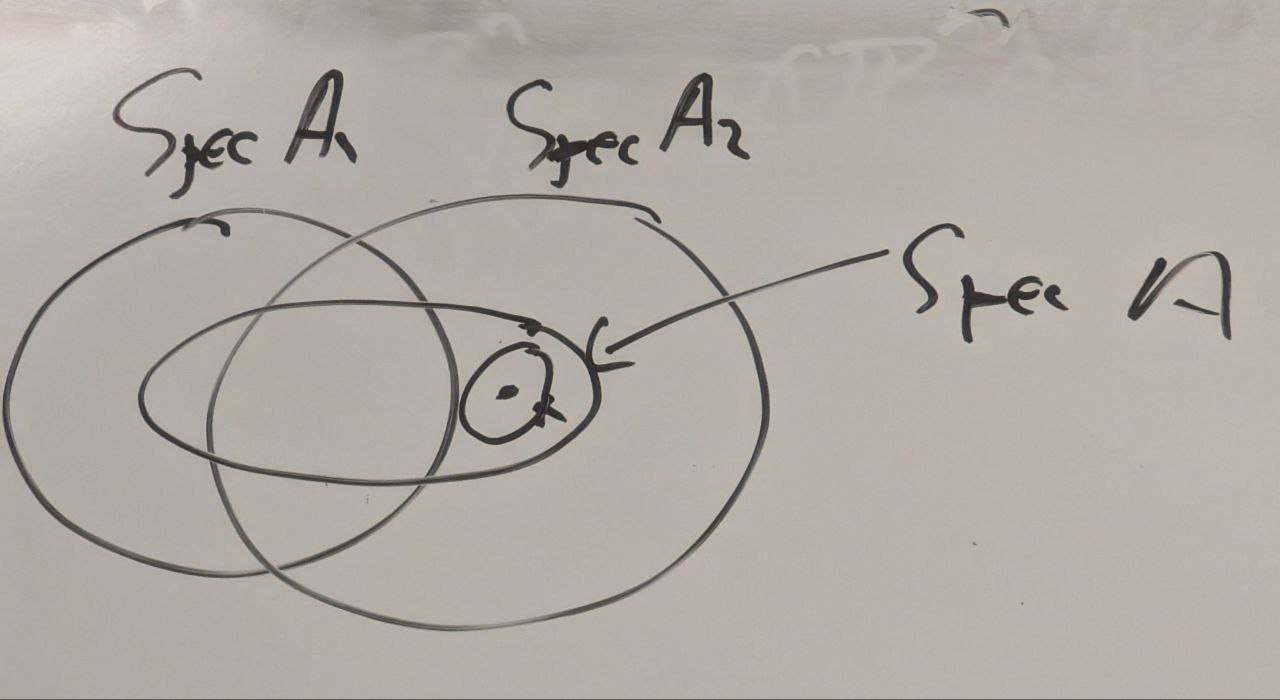
\includegraphics[width=0.8\textwidth]{img/commlemma}
            \caption{Claim}
        \end{figure}

        We omit the proof of the claim for now.

        Then this open set \(\operatorname{Spec} A_{f_x}\) has property \(P\) from \(\operatorname{Spec} A_i\). \(\bigcup_{x\in \operatorname{Spec} A} \operatorname{Spec} A_{f_x} = \operatorname{Spec} A\).

        So \(\operatorname{Spec} A = \operatorname{Spec} A_{f_{x_1}} \cup \cdots \cup \operatorname{Spec} A_{f_{x_n}}\).
        
        Since \((f_{x_1}, \cdots , f_{x_n}) = (1)\) we deduce that \(\operatorname{Spec} A\) has property \(P\).
    \end{proof}

    \begin{lemma}
        Let \(\operatorname{Spec} A, \operatorname{Spec} B\) denote open affine subsets of \(\operatorname{Spec} X\). Suppose \(x\in \operatorname{Spec} A\cap \operatorname{Spec} B\).

        Then \(x\) has an affine open neighborhood which is distinguished in both \(\operatorname{Spec} A\) and \(\operatorname{Spec} B\).
    \end{lemma}

    \begin{proof}
        A distinguished open subset of a distinguished open subset is distinguished.

        \(D(\operatorname{Spec} A, f)\)

        \(D\left(\operatorname{Spec} A \left[ \frac{1}{f} \right], \frac{g}{f^n}\right)\) 

        \(D(\operatorname{Spec} A, fg)\)

        So we may replace \(\operatorname{Spec} B\) by an open neighborhood of \(x\), \(D(\operatorname{Spec} B, g)\) which is contained in \(\operatorname{Spec} A \cap \operatorname{Spec} B\). Thus we can assume \(\operatorname{Spec} B \subset \operatorname{Spec} A\).

        We can take \(D(\operatorname{Spec} A, f)\) a neighborhood of \(x\) inside \(\operatorname{Spec} B\).

        \(f\in A = \Gamma (\operatorname{Spec} A, \mathcal{O}_X) \xrightarrow{\operatorname{Res}} \Gamma(\operatorname{Spec} B, \mathcal{O}_X) = B\).

        So \(\operatorname{Res}(f) = f^{\prime} \in B\).

        Claim: \(D(\operatorname{Spec} B, f^{\prime}) = D(\operatorname{Spec} A, f)\).

        This finishes the proof.

    \end{proof}

    \section*{Monday, 10/13/2025}
    
    Recall affine communication lemma: given a ring property \(P\) such that:

    \begin{enumerate}[label=\arabic*)]
        \item If \(A\) has \(P\) then \(A \left[ \frac{1}{f} \right] \) has \(P\).
        \item If \(f_1, \cdots , f_n \in A, (f_1, \cdots , f_n) = (1)\) and \(A \left[ \frac{1}{f_i} \right] \) has \(P\) then \(A\) has \(P\). 
    \end{enumerate} 

    then every scheme \(X\) with an affine open cover by \(\operatorname{Spec} A_\alpha\) where \(A_\alpha\) all have \(P\) has the property that every affine open \(\operatorname{Spec} B \subset X, B\) has \(P\).

    In this case we say \(X\) locally has property \(P\).

    Furthermore, if \(X\) is quasi-compact [so it has a finite affine open cover] then \(X\) has \(P\). i.e. If \(X\) is quasi-compact, then \(X\) having a property locally implies \(X\) has the property.

    Examples: Let \(P =\) Noetherian. First we verify:

    \begin{proposition}
        If \(f\in A\) and \(A\) is Noetherian then \(A[1 / f]\) is Noetherian. 
    \end{proposition}

    \begin{proof}
        Easy using Hilbert Basis Theorem: \(A [ 1 / f] = A [x] / (fx - 1)\). Hilbert Basis Theorem implies \(A[x]\) is Noetherian, and any quotient of a Noetherian ring is Noetherian.
    \end{proof}

    \begin{proposition}
        If \(f_1, \cdots , f_n \in A\) generate \((1)\) and each \(A[1 / f_i]\) is Noetherian then \(A\) is Noetherian.
    \end{proposition}

    \begin{proof}
        Let \(I_1 \subset I_2 \subset I_3 \subset\) an ascending chain of ideals of \(A\).

        Fix \(i\). \(I_1[1 / f_i] \subset I_2[1 / f_i] \subset \cdots\) is an ascending chain of ideals in \(A [1 / f_i]\). Noetherian implies they eventually stabilize. Since there are finitely many \(f_i\) then \(\exists N\) such that \(\forall m > N, \forall i, I_m [1 / f_i] = I_{m+1} [1 / f_i]\).

        Claim: \(\forall m > N, I_m = I_{m+1}\) [so the original chain of ideal stabilizes].

        Proof: \(I_{m+1} / I_m\) is an \(A\)-module. Now consider \((I_{m+1} / I_m) [1 / f_i]\). We claim that \((I_m / I_{m+1}) \cong I_{m+1} [1 / f_i] / I_m [1 / f_i]\).
        
        To see this, consider the SES:

        \[
            0 \to I_m \to I_{m+1} \to I_{m+1} / I_m \to 0
        \]

        Flatness of localization implies:

        \[
            0 \to I_m [1 / f_i] \to I_{m+1} [1 / f_i] \to (I_{m+1} / I_m) [1 / f_i] \to 0
        \]

        When is \(S ^{-1} M = (0)\)? when \(\forall m, \exists s \in S\) such that \(sm = 0\).

        If \(x\in I_{m+1}\) representing a class in \(I_{m+1} / I_m\) then \(\forall i, \exists k_i\) such that \(f_i^{k_i} x = 0\) in \(I_{m+1} / I_m\). \(\exists k\) such that \(f_i^k x \in I_m\). Write \(1 = \sum_{i=1}^n c_i f_i\).

        \(1 = 1^{nk} = \left( \sum_{i=1}^n c_i f_i \right)^{nk} = \sum_{i=1}^n d_i f_i^k\).
        
        \(\implies x = \sum_{i=1}^n d_i x f_i^k \in I_m\).

    \end{proof}

    \begin{corollary}
        Every locally Noetherian scheme is quasiseparated.
    \end{corollary}

    \begin{proof}
        Let \(\operatorname{Spec} A, \operatorname{Spec} B\) be affine open in \(X\). We are interested in \(\operatorname{Spec} A \cap \operatorname{Spec} B \subset \operatorname{Spec} A =\) Noetherian topological space. Open subset of Noetherian topological space must be Noetherian. So \(\operatorname{Spec} A \cap \operatorname{Spec} B\) must also be Noetherian.

        Noetherian spaces are quasicompact. 
    \end{proof}

    Current notion of scheme is built up by spectra of commutative ring, and a commutative ring is the same thing as a \(\mathbb{Z}\)-algebra. A sheaf of commutative ring is a shief of \(\mathbb{Z}\)-algebras. We can thus generalize the notion of schemes:

    \begin{definition}
        [\(A\)-scheme] If \(A\) is any commutative ring, then an \(A\)-scheme is a ringed space, i.e. a pair \(X, \mathcal{O}_X\) consisting of a space  and a sheaf of \(A\)-algebras with the property that \(X\) has a cover by \(\operatorname{Spec} B_\alpha\) where \(B_\alpha\) are \(A\)-algebras.
    \end{definition}

    An \(A\)-scheme is the same thing as a scheme \(X\) with a morphism to \(\operatorname{Spec} A\).

    Now, property \(P\) is no longer necessarily a property of a ring, it is rather property of \(A\)-algebra.

    We write \(P_A\) to be a property of \(A\)-algebra.
    
    Let \(P_A\) be the property \(B\) is a finitely generated \(A\)-algebra.

    Any finitely generated \(A\)-algebra can be thought of as a quotient of a polynomial ring over \(A\). So finitely generated \(A\)-algebras are noetherian. \(P_A\) satisfies the conditions for the affine communication lemma.

    \begin{lemma}
        If \(B\) is finitely generated over \(A\) then \(B[1 / f]\) is finitely generated over \(A\).
    \end{lemma}

    \begin{proof}
        \(B[1 / f] = B[x] / (fx - 1)\).
    \end{proof}

    \begin{theorem}
        Suppose \(B\) is an \(A\)-algebra and \(f_1, \cdots , f_n\in B\) generating the unit ideal, and each \(B[1 / f_i]\) is a finitely generated \(A\)-algebra. Then \(B\) is a finitely generated \(A\)-algebra.
    \end{theorem}

    \begin{proof}
        \(\forall f_i \exists\) generators \(\frac{b_{i,j}}{f_i^{N_{i,j}}}\) of \(B[1 / f_i]\). We have \(\sum_{i=1}^n c_i f_i = 1\). Assume WLOG all \(N_{i,j} = N\) for some fixed \(N\). 

        Claim: \(\{ f_i \} \cup \{ c_i \} \cup \{ b_{i,j} \} \) generate \(B\).

        Proof: Given \(b\in B\), for each \(f_i\) we can write \(b \in B[1 / f_i]\) as a polynomial in \(b_{ij} / f_i^N\).

        Clearing the denominator, WLOG for some big \(M_i\), we can write \(b f_i^{M_i}\) as a polynomial in \(b_{i,j}\) together with \(f_i\).
        
        WLOG \(M_i = M\) for some large \(M\).

        Then \(b f_i^M \in A[b_{i,j}, f_i]\).

        \(\sum_{i} c_i f_i = 1 \implies \left( \sum_{i} c_i f_i \right)^{Mn} = 1 \implies d_i f_i^M = 1, d_i \in A[c_1, \cdots , c_n, f_1, \cdots , f_n]\).

        Thus \(b = \sum_{i} d_i b f_i^M \in A[c_i, f_i, b_{i,j}]\).
    \end{proof}

    \begin{definition}
        [Harthshorne] Let \(X\) be a \(k\)-scheme where \(k = \overline{k}\). Then \(X\) is a \(k\)-variety means that \(X\) is integral, separated and of finite type.
    \end{definition}

    \begin{definition}
        [Vakil] A \(k\)-scheme \(X\) is a \(k\)-variety means \(X\) is reduced, separated, and of finite type.
    \end{definition}

    Why does Harthshorne restrict to algebraically closed fields? Base change in algebraic geometry lets us turn \(A\)-schemes to \(B\)-schemes. It might happen that if we go from a field to a field extension, we can lose the property of being irreducible: see \(\mathbb{C} \otimes_\mathbb{R} \mathbb{C}\). Harthshorne doesn't want to worry about that. A lot of authors want to follow Harthshorne, so when they define \(k\)-scheme they want to restrict to the case where we don't have problem if we base change to \(\overline{k}\).

    Let \(k\) be a field, \(X\) a \(k\)-scheme which is locally of finite type and \(x\in X\) a closed point. Then we can define the degree \(\deg(x)\) as follows:

    \(\mathbb{K} (x) = \mathcal{O}_{X,x} / \mathfrak{m}\) is a field which is also a \(k\)-vector space. i.e. \(\mathbb{K} (x) / k\) is a field extension. Then \(\deg(x)\) is the degree of the field extension. Why should it be a finite extension?
    
    \(X\in \operatorname{Spec} A \subset X, A\) is a finitely generated \(k\)-algebra.

    Note that \(\mathbb{K} (x) = A_{\mathfrak{m}} / \mathfrak{m}_{\mathfrak{m}} = A / \mathfrak{m}\).

    As a ring, \(\mathbb{K} (x)\) is finitely generated over \(k\). By the Nullstellensatz, \(\mathbb{K} (x)\) is a finite extension of \(k\).

    Example: Suppose \(k=\mathbb{R}, X = \operatorname{Spec} k[x,y] / (x^2 + y^2 - 1)\). This is the circle in \(\mathbb{R}^2\). Consider a point on the circle, let's say \((3 / 5, 4 / 5)\). This corresponds to the ideal \(I = (x - 3 / 5, y - 4 / 5)\). This is a degree \(1\) point.

    If we take \((2, \pm \sqrt{-3})\), then we get the ideal \((x-2, y^2 + 3)\) which has degree \(2\).
    
    It roughly tracks what happens if we change base to a field extension.

    Now, suppose we have \(A\) an integral domain. \(A \subset K = A_{(0)}\). Consider a monic polynomial \(x^n + a_1 x^{n-1} + \cdots + a_n\) with \(a_i \in A\). Since \(A\) might not be \(\mathbb{Z}\), we might have a root in \(K\) that is not in \(A\). This doesn't happen in \(\mathbb{Z}\). This can be captured by normality. A self intersecting curve doesn't have normality, for example.

    \section*{Wednesday, 10/15/2025}
    
    Let \(A\) be an integral domain, \(K = \operatorname{Frac} (A)\).

    \(A\) is integrally closed means that every root in \(K\) of any monic polynomial in \(A\) lies in \(A\).

    For example \(\mathbb{Z}\) is integrally closed:

    Suppose \(a,b\in \mathbb{Z} \) and \(\frac{a}{b}\) is a root of \(x^n + c_1 x^{n-1} + \cdots + c_n\) with \(c_i\in \mathbb{Z}\). Further suppose \(\frac{a}{b}\) is written in lowest terms, i.e. \(\gcd(a,b)=1\).

    \[
        \left( \frac{a}{b} \right)^n + c_1 \left( \frac{a}{b} \right)^{n-1} + \cdots + c_n = 0
    \]

    Clearing denominators,

    \[
        a^n + c_1 a^{n-1} b + \cdots + c_n b^n = 0
    \]

    So \(b\mid a^n\). Thus a prime factor of \(b\) must be a prime factor of \(a\), so \(b=1\).

    We only used the fact that \(\mathbb{Z}\) is a UFD. We can deduce:

    \begin{theorem}
        Every UFD is integrally closed.
    \end{theorem}

    In particular, note that polynomial ring over UFD is UFD.

    Non example: let \(A = k[t^2, t^3] = \operatorname{Span}_k (1, t^2, t^3, t^4, \cdots)\). Then \(\operatorname{Frac} (A) = k(t)\). \(t\) is a root of \(x^2 - t^2\).

    \begin{proposition}
        If \(A\) is integrally closed and \(S\) is a mutiplicative system in \(A\), then \(S ^{-1} A\) is integrally closed.
    \end{proposition}

    \begin{proof}
        Let \(x^n + c_1 x^{n-1} + \cdots + c_n \in S ^{-1} A [x]\).

        We can write \(c_i = \frac{d_i}{s^i}\) for some \(s\in S\).

        Let \(\alpha \in \operatorname{Frac} (S ^{-1} A) = \operatorname{Frac} (A)\) be a root of this polynomial.

        Then \(s \alpha\) is a root of \(x^n + d_1 x^{n-1} + \cdots + d_n\).

        Thus \(s \alpha \in A \implies \alpha \in S ^{-1} A\).
    \end{proof}

    \begin{corollary}
        If \(A\) is integrally closed and \(P\) is a prime ideal in \(A\) then the local ring \(A_P\) is integrally closed.
    \end{corollary}

    The (right) converse is also true.

    \begin{proposition}
        If \(A\) is an integral domain and \(A_P\) is integrally closed for all prime ideals \(P\) of \(A\) then \(A\) is integrally closed. 
    \end{proposition}

    \begin{proof}
        Let \(K = \operatorname{Frac} (A)\). Suppose \(\alpha \in K\) is the root of a monic polynomial with coefficients in \(A\). Let \(I = \{ a\in A \mid a \alpha \in A \}\). This is an ideal.

        If \(I = A\) then \(1\in I \implies \alpha \in A\) so we're done.

        Note that if \(\alpha \neq 0\) we have \(I\neq 0\).

        Now suppose \(I\) is a proper ideal.

        Let \(\mathfrak{m} \subset A\) be a maximal ideal containing \(I\).

        Claim: \(\alpha \notin A_{\mathfrak{m}}\). Suppose otherwise. Then \(\alpha = \frac{t}{m}\) where \(m\in A\setminus  \mathfrak{m} \) but \(m \alpha \in A \implies m\in I \subset \mathfrak{m} \).   

        However, \(A_{\mathfrak{m}}\) is integrallly closed and contains \(A\). Contradiction.
    \end{proof}

    \begin{definition}
        \(X\) is a \textit{normal scheme} if it is irreducible and every \(\mathcal{O}_{X,x}\) is integrally closed.
    \end{definition}

    \begin{theorem}
        TFAE:

        \begin{enumerate}[label=\arabic*)]
            \item \(X\) is normal.
            \item \(X\) is irreducible and has an affine cover.
            \item \(X\) is irreducible and every affine open is the spectrum of an integrally closed ring. 
        \end{enumerate} 
    \end{theorem}

    \subsection*{Chapter 6: Quasicoherent Sheaves}

    \((X, \mathcal{O}_X)\).

    A sheaf \(\mathcal{F}\) of \(\mathcal{O}_X\)-modules means a sheaf of abelian groups with for each \(U \subset X\), an \(\mathcal{O}_X(U)\)-module structure on \(\mathcal{F} (U)\) compatible with restriction maps.
    
    Quasicoherent sheaves are the main and most important class of \(\mathcal{O}_X\)-modules.

    Let \(A\) be a commutative ring, \(M\) an \(A\)-module. Set \(X = \operatorname{Spec} A\). We define \(\widetilde{M}\) to be a sheaf of \(\mathcal{O}_X\)-modules satisfying:
    
    \[
        \widetilde{M}(D(f)) = M \left[ \frac{1}{f} \right]
    \]

    Note that \(M \left[ \frac{1}{f} \right] \) is a module over \(\mathcal{O}_X(D(f)) = A \left[ \frac{1}{f} \right]\).

    One of the ways to define a sheaf are on a base, and distinguished open sets form a base.

    The modules of this form are called \textit{quasicoherent}.

    What are the stalks of this sheaf?

    \(\widetilde{M}_P = M_P\).

    Let \((f_1, \cdots , f_n) = (1)\). i.e. \(\operatorname{Spec} A = \bigcup_{i=1}^n D(f_i) \).

    We have the exact sequence (proved earlier):

    \[
        0 \to A \to \bigoplus_{1 \leq i \leq n} A \left[ \frac{1}{f_i} \right] \to \bigoplus_{1 \leq i \neq j \leq n} A \left[ \frac{1}{f_i f_j} \right]  
    \]

    It generalizes to modules:

    \[
        0 \to M \to \bigoplus_{1 \leq i \leq n} M \left[ \frac{1}{f_i} \right] \to \bigoplus_{1 \leq i \neq j \leq n} M \left[ \frac{1}{f_i f_j} \right]  
    \]

    Now we can define quasicoherent sheaves in general.

    \begin{definition}
        A sheaf \(\mathcal{F}\) of \(\mathcal{O}_X\)-modules on \(X\) is \textit{quasicoherent} if and only if there exists an affine cover of \(X\) given by \(\bigcup_{\alpha \in I} \operatorname{Spec} A_\alpha\) and a collection of \(A_\alpha\)-modules \(M_\alpha\) such that,

        \[
            \eval{\mathcal{F}}_{\operatorname{Spec} A_\alpha} \text{ as a module over } \mathcal{O}_{\operatorname{Spec} A_\alpha} \cong \widetilde{M}_\alpha
        \]
    \end{definition}

    \begin{theorem}
        The map \(M \mapsto \widetilde{M}\) gives an equivalence of categories from \(A\)-modules to quasicoherent \(\mathcal{O}_{\operatorname{Spec} A}\)-modules. 
    \end{theorem}

    \begin{proof}
        Check: morphisms are the same.

        Let \(M,N \in \operatorname{Mod}_A\), \(\phi : M\to N\) an \(A\)-linear map.

        Define \(\widetilde{\phi}: \widetilde{M} \to \widetilde{N}\) by,

        \[
            \widetilde{\phi} (D(f)): \widetilde{M} (D(f)) = M \left[ \frac{1}{f} \right] \to \widetilde{N}(D(f)) = N \left[ \frac{1}{f} \right]
        \]

        \[
            \frac{m}{f^k} \mapsto \frac{\phi(m)}{f^k}
        \]

        The main thing to check: 

        Claim: If \(\psi: \widetilde{M} \to \widetilde{N}\) is a morphism of \(\mathcal{O}_{\operatorname{Spec} A}\)-modules there exists unique \(\phi: M \to N\) such that \(\psi = \widetilde{\phi}\).

        Proof of Claim: note that \(\psi (\operatorname{Spec} A): \widetilde{M} (\operatorname{Spec} A) \to \widetilde{N} (\operatorname{Spec} A)\) but \(\widetilde{M} (\operatorname{Spec} A) = M, \widetilde{N} (\operatorname{Spec} A) = N\) so we have \(M \to N\) given by \(\phi\). We claim that \(\psi = \widetilde{\phi}\).

        \[
            \begin{tikzcd}
                \widetilde{M} (\operatorname{Spec} A) \ar[r] \ar[d] & \widetilde{N} (\operatorname{Spec} A) \ar[d] \\ \widetilde{M} (D(f)) \ar[r] & \widetilde{N} (D(f))
            \end{tikzcd}
        \]

        \[
            \begin{tikzcd}
                m \ar[d, mapsto] & M \ar[r,"\phi"] \ar[d] & N \ar[d] & n \ar[d, mapsto] \\ \frac{m}{1} & M \left[ \frac{1}{f} \right] \ar[r] & N \left[ \frac{1}{f} \right] & \frac{n}{1} \\ & \phi \left( \frac{m}{1} \right) \ar[r,"=", phantom] & \frac{\phi(m)}{1}
            \end{tikzcd}
        \]
    \end{proof}

    \begin{theorem}
        If \(\mathcal{F}\) is an \(\mathcal{O}_X\) module which is quasicoherent w.r.t.\ some affine cover, then it is quasicoherent w.r.t.\ all affine opens.
    \end{theorem}

    \begin{proof}
        We use affine communication lemma. Need to check:

        \begin{enumerate}[label=\arabic*)]
            \item If \(\mathcal{F}\) is quasicoherent on \(\operatorname{Spec} A\) then \(\eval{\mathcal{F}}_{D(f)}\) is quasicoherent on \(\operatorname{Spec} A\left[ \frac{1}{f} \right]\):
            
            \(\eval{\widetilde{M}}_{D(f)} (D(fg)) = \widetilde{M} (D(fg)) = M \left[ \frac{1}{fg} \right]\). So \(\eval{\widetilde{M}}_{D(f)} = \widetilde{M \left[ \frac{1}{f} \right] }\).   

            \item Suppose now \(\mathcal{F}\) is a sheaf of \(\mathcal{O}_{\operatorname{Spec} A}\)-modules on \(\operatorname{Spec} A\), \(f_1, \cdots , f_n \in A\) with \((f_1, \cdots , f_n) = 1\) and for each \(i\) we have \(A \left[ \frac{1}{f_i} \right] \)-module \(M_i\) such that \(\eval{\mathcal{F}}_{D(f_i)} \cong \widetilde{M}_i\). Then we want to show that \(\exists\) an \(A\)-module \(M\) such that \(\mathcal{F} \cong \widetilde{M}\) as \(\mathcal{O}_{\operatorname{Spec} A}\)-module:
            
            Main task is figuring out what \(M\) is.

            \[
                \begin{tikzcd}
                    & \eval{\mathcal{F}}_{D(f_i f_j)} \ar[ld, "\cong"] \ar[rd,"\cong"] \\ \eval{\widetilde{M}_i}_{D(f_i f_j)} \ar[rr,"\cong"] \ar[d,"="] & & \eval{\widetilde{M}_j}_{D(f_i f_j)} \ar[d,"="] \\
                    \widetilde{M_i \left[ \frac{1}{f_j} \right]} \ar[rr, "\widetilde{\Phi}_{ij}", "\cong"'] & & \widetilde{M_j \left[ \frac{1}{f_i} \right]} 
                \end{tikzcd}
            \]

            \(\widetilde{\Phi}_{ij}\) must come from some \(\Phi_{ij}: M_{i,j} = M_i \left[ \frac{1}{f_j} \right] \xrightarrow{\cong} M_j \left[ \frac{1}{f_i} \right] = M_{j,i}\). 
            
            \[
                M \coloneqq \ker \bigoplus_{1 \leq i \leq n} M_i \to \bigoplus_{1 \leq i \neq j \leq n} M_{i,j} 
            \]

            To prove that \(\mathcal{F} \cong \widetilde{M} \) the main thing is to prove that \(\forall i\),

            \[
                \widetilde{M}_i = \eval{\widetilde{F}}_{D(f_i)} \xrightarrow{\sim} \eval{\widetilde{M}}_{D(f_i)}
            \]

            Comparing two quasi-coherent sheaves on \(D(f_i)\).

            So we're checking \(M_i \xrightarrow{\sim} M \left[ \frac{1}{f_i} \right]\).

            WLOG we check \(M_1 \xrightarrow{\sim} M \left[ \frac{1}{f_1} \right]\).

            Localization is exact. So,

            \[
                0 \to M \to \bigoplus_{i} M_i \to \bigoplus_{i\neq j} M_{i,j} 
            \]

            \[
                0 \to M\left[ \frac{1}{f_1} \right]  \to \bigoplus_{i} M_i \left[ \frac{1}{f_1} \right] = M_{i1} \to \bigoplus_{i\neq j} M_{i,j} \left[ \frac{1}{f_1} \right]   
            \]

            \[
                0 \to M_1 \to \bigoplus_{i} M_{i,1} \to \bigoplus_{i\neq j} M_{i,j,1}
            \]

        \end{enumerate} 
    \end{proof}

    \section*{Friday, 10/17/2025}
    
    \(X = \operatorname{Spec} A, \mathcal{F}\) is an \(\mathcal{O}_X\)-module.

    \(X = \bigcup_{i=1}^n D(f_i), \eval{\mathcal{F}}_{D(f_i)} \cong \widetilde{M}_i\).

    \(M_i\) is an \(A[1 / f_i]\)-module.

    Claim: \(\exists\) an \(A\)-module \(M\) such that \(\mathcal{F} \cong \widetilde{M}\).

    \[
        \widetilde{M_i[1 / f_j]} = \eval{\widetilde{M}_i}_{D(f_i f_j)} \cong \eval{\mathcal{F}}_{D(f_i f_j)} \cong \eval{\widetilde{M}_j}_{D(f_i f_j)} = \widetilde{M_j[1 / f_i]}  
    \]

    \[
        \Phi_{i,j} M_i[1 / f_j] \xrightarrow{\sim} M_j[1 / f_i] = M_{i,j} 
    \]

    Let \(M = \ker \gamma\) in the following:

    \[
        0 \to M \to \bigoplus_{i=1}^n M_i \xrightarrow{\gamma} \bigoplus_{1 \leq i\neq j \leq n} M_{i,j}
    \]

    We need: \(\widetilde{M}_{D(f_i)} (= \widetilde{M[1 / f_i]}) \cong M_i\).

    Claim: \(M[1 / f_i] \cong M_i\). WLOG \(i = 1\).

    \[
        \begin{tikzcd}
            0 \ar[r] & M[1 / f_1] \ar[d, dotted] \ar[r] & \bigoplus_{i=1}^n M_i[1 / f_1] \ar[d,"\cong", "{\Phi_{i,1}}"'] \ar[r] & \bigoplus_{1 \leq i\neq j \leq n} M_{i,j} [1 / f_1] \ar[d,"\cong", "{\Phi_{i,1}[1 / f_j]}"'] \\ 0 \ar[r] & M_1 \ar[r] & \bigoplus_{i=1}^n M_1[1 / f_i] \ar[r,"\gamma_{M_1}"] & \bigoplus_{1 \leq i\neq j \leq n} M_1[1 / f_i f_j]     
        \end{tikzcd}
    \]

    If \(\mathcal{F}\) is quasicoherent then \(\mathcal{F} (\operatorname{Spec} A) = M\).

    [missed some stuff here]

    \(\operatorname{Res}^{D(f)}_{\operatorname{Spec} A}: M \to M^{\prime}\) is \(A\)-linear.
    
    By universal property of localization,

    \[
        \begin{tikzcd}
            M \ar[rr] \ar[rd] & & M^{\prime} \\ & M[1 / f] \ar[ru, dotted]
        \end{tikzcd}
    \]

    \(M[1 / f] \to M^{\prime}\) exists for all \(\mathcal{O}_X\)-modules.
    
    If \(\mathcal{F}\) is a sheaf of \(\mathcal{O} _X\)-modules and for all afine opens \(\operatorname{Spec} A \subset X\) and all distinguished opens \(D(f) \subset \operatorname{Spec} A\) we have:

    \[
        \mathcal{F} (\operatorname{Spec} A)[1 / f] \to \mathcal{F} (D(f))
    \]

    is an isomorphism is an isomorphism of \(A[1 / f]\) modules then \(\mathcal{F} \) is quasicoherent.

    \subsection*{Tensor Products}

    Let \(\mathcal{F} , \mathcal{G}\) be \(\mathcal{O}_X\) modules.

    There is a presheaf tensor product given by \(\mathcal{F} \otimes_{\mathcal{O}_{X,\text{pre}}}(U) = \mathcal{F}(U) \otimes_{\mathcal{O}_X(U)} \mathcal{G}(U)\).
    
    Suppose we have \(M,N\) \(A\)-modules and \(f:M \to M^{\prime} , g:N \to N^{\prime} , h:A \to A^{\prime} \).

    \(F:M \otimes_A N \to M^{\prime} \otimes_{A^{\prime}} N^{\prime}\) then \(m \otimes n \mapsto f(m) \otimes g(n)\) and we extend by linearity.
    
    \(F(am \otimes n) = h(a)f(m)\otimes g(n) = f(m) \otimes h(a)g(n) = f(m) \otimes g(an) = F(m \otimes an)\).
    
    Let \(\mathcal{F} , \mathcal{G} \text{ be } \mathcal{O}_X\)-modules.

    
    \[
        \mathcal{F} \otimes_{\mathcal{O}_{X,pre}} \mathcal{G} (U) = \mathcal{F}(U) \otimes_{\mathcal{O}_X(U)} \mathcal{G}(U)
    \]

    \[
        \mathcal{F} \otimes_{\mathcal{O}_X} \mathcal{G} = (\mathcal{F} \otimes_{\mathcal{O}_{X,pre}} \mathcal{G}) ^{\operatorname{sh}}
    \]

    \((\mathcal{F} \otimes_{\mathcal{O}_X} \mathcal{G})_x = \mathcal{F}_x \otimes_{\mathcal{O}_{X,x}} \mathcal{G}_x\).

    If \(\mathcal{F} , \mathcal{G} \) are quasicoherent then \(\mathcal{F} \otimes \mathcal{G}\) is again quasicoherent.

    Let \(\operatorname{Spec} A\) be affine open, \(D(f)\) a distinguished open of \(\operatorname{Spec} A\). 

    \(\mathcal{F} = \widetilde{M} , \mathcal{G} = \widetilde{N}\) where \(M,N\) are \(A\)-modules.

    Define a sheaf \(\mathcal{H} = \widetilde{M \otimes_A N}\).
    
    There is a natural map of \(\mathcal{O}_X\)-module \(\mathcal{F} \otimes_{pre} \mathcal{G} \to \mathcal{H}\).

    \(D(f) \subset \operatorname{Spec} A \subset X\).

    \(\eval{\mathcal{F}}_{\operatorname{Spec} A} = \widetilde{M}, \eval{\mathcal{G}}_{\operatorname{Spec} A} = \widetilde{N}\).
    
    \[
        \eval{\mathcal{H}}_{\operatorname{Spec} A}  = \widetilde{M \otimes_A N} 
    \]

    this defines a quasicoherent sheaf because:

    \[
        \eval{\mathcal{H}}_{\operatorname{Spec} A[1 / f]} = M[1 / f] \otimes_{A[1 / f]} N[1 / f]
    \]

    \[
        \simeq (M \otimes_A N)[1 / f]
    \]

    \[
        \frac{m}{f^k} \otimes \frac{n}{f^l} \mapsto \frac{m \otimes n}{f^{k+l}}
    \]

    We can check stalk level:

    \[
        \mathcal{H}_x = \mathcal{F}_x \otimes_{\mathcal{O}_{X,x}} \mathcal{G}_x
    \]

    Let \(X\) be any scheme, \(\mathcal{F}\) a sheaf of \(\mathcal{O}_X\)-modules.

    Let \(f \in \Gamma(X, \mathcal{O}_X)\). Then \(X_f = \{ x\in X \mid f(x) \neq 0 \} \).

    \(X_f\) is open so we can talk about \(\Gamma (X_f, \mathcal{O}_X)\).

    \[
        \begin{tikzcd}
            \Gamma (X, \mathcal{O}_X) \ar[rr] \ar[rd] & & \Gamma (X_f, \mathcal{O}_X) \\ & \Gamma (X, \mathcal{O}_X)[1 / f] \ar[ur, dotted]
        \end{tikzcd}
    \]


    \begin{lemma}
        [QCQS Lemma] If \(X\) is QCQS (quasicompact quasiseparated) then \(\mathcal{F}\) is quasicoherent if and only if the map in the above diagram \(\Gamma (X, \mathcal{O} _X)[1 / f] \to \Gamma(X_f, \mathcal{O}_X)\) is an isomorphism for all \(f\).
    \end{lemma}

    If \(X\) is QCQS then it has a finite open cover \(X = \bigcup_{i} \operatorname{Spec} A_i\) such that each \(\operatorname{Spec} A_i \cap \operatorname{Spec} A_j = \bigcup_{k} \operatorname{Spec} B_{i,j,k}\).

    We can look at the sequence:

    \[
        0 \to \Gamma (X, \mathcal{F}) \to \bigoplus_{i} \Gamma (\operatorname{Spec} A_i, \mathcal{F}) \xrightarrow{\gamma} \bigoplus_{i,j,k} \Gamma (\operatorname{Spec} B_{i,j,k}, \mathcal{F})
    \]

    [then not clear, later]

    \subsection*{Gorthendieck Pretopologies}

    Regularly, we have the set of affines, some collections of smaller affinees from good covers.

    In a Grothendieck pretopology we have a collections of open sets \(U\) and for each \(U\) a collection of covers, which are sets of open sets contained in \(U\).

    But we don't want to think of these as sets, these can be objects in a category. So actual axioms are different.

    \begin{enumerate}[label=\arabic*)]
        \item If \(\{ U_i \} \) is a cover of \(U\) and \(V \subset U\) is any open subset then \(\{ U_i\cap V \} \) is a cover of \(V\). 
        \item If \(\{ U_i \} \) is a cover of \(U\) and for each \(i\), \(\{ U_{i,j} \} \) is a cover of \(U_i\) then \(\{ U_{i,j}  \} \) is a cover of \(U\).
        \item \(\{ U \}\) is a cover of \(U\). 
    \end{enumerate} 

    If we think about distinguished opens,

    \begin{enumerate}[label=\alph*)]
        \item Every \(U\) is a distinguished open of itself.
        \item If \(V\) is a distinguished open of \(U\) and \(W\) is a distinguished open of \(U\) then \(V \cap W\) is a distinguished open of \(V\) and \(W\) itself. 
    \end{enumerate} 

    \section*{Monday, 10/20/2025}
    
    We review the QCQS [Quasicompact Quasiseprated] lemma
    
    \begin{lemma}
        [QCQS Lemma] Let \(X\) be a QCQS scheme. If \(\mathcal{F}\) is a quasicoherent sheaf of \(\mathcal{O}_X\)-mod and \(f\in \Gamma(X, \mathcal{O}_X)\) and \(X_f = \{ x\in X \mid f(x)\neq 0 \} \) an open subset of \(X\),

        \[
            \Gamma(X, \mathcal{F}) \left[ \frac{1}{f} \right] \xrightarrow{\sim} \Gamma(X_{f}, \mathcal{F}).
        \]
    \end{lemma}

    Let \(X = \bigcup_{i=1}^n U_i\) where \(U_i = \operatorname{Spec} A_i\).

    We can write \(U_i \cap U_j = \bigcup_{k=1}^{n_{i,j}} U_{i,j,k}\) where \(U_{i,j,k} = \operatorname{Spec} A_{i,j,k}\).

    \(\eval{\mathcal{F}}_{U_i} = \widetilde{M}_i\) and \(\eval{\mathcal{F}}_{U_{i,j,k}} = \widetilde{M}_{i,j,k}\).
        
    Sheaf axioms:

    \[
        0 \to \Gamma(X,\mathcal{F}) \to \bigoplus_{i=1}^n \Gamma(U_{i}, \mathcal{F}) \to \bigoplus_{i,j,k} \Gamma (U_{i,j,k}, \mathcal{F})
    \]

    Sequence of \(\Gamma (X , \mathcal{O}_X)\)-modules.

    Apply \((f^{\mathbb{Z}}) ^{-1}\) to the complex. Recall \(\bigoplus \Gamma (U_i , \mathcal{F}) = \bigoplus M_i\) and \(\bigoplus \Gamma (U_{i,j,k} ,\mathcal{F}) = \bigoplus M_{i,j,k}\).
        
    We have,
        
    \[
       0 \to \Gamma(X, \mathcal{F})\left[ \frac{1}{f} \right] \to \bigoplus_{i} M_i \left[ \frac{1}{f} \right] \to \bigoplus_{i,j,k} M_{i,j,k} \left[ \frac{1}{f} \right] 
    \]

    \[
        0 \to \Gamma(X_f , \mathcal{F}) \to \bigoplus_{i} \Gamma (X_f \cap U_i , \mathcal{F}) \to \bigoplus_{i,j,k} \Gamma (X_f \cap U_{i,j,k} , \mathcal{F})
    \]

    Intermission: when is a full subcategory of an abelian category abelian?

    A full subcategory \(\mathcal{D}\) of an abelian category \(\mathcal{C}\) is an abelian category if and only if:

    \begin{enumerate}[label=\arabic*)]
        \item \(0\in \mathcal{D}\).
        \item \(\forall X , Y \in \mathcal{D}, X \oplus Y \in \mathcal{D}\).
        \item \(\forall X,Y \in \mathcal{D}, \phi \in \operatorname{Hom}_{\mathcal{C}}(X,Y) = \operatorname{Hom}_{\mathcal{D}}(X,Y)\), we must have \(\ker \phi, \operatorname{coker} \phi \in \mathcal{D}\).  
    \end{enumerate} 

    \begin{theorem}
        For any scheme \(X\), the category \(\operatorname{Qcoh}_X\) is abelian.
    \end{theorem}

    \begin{proof}
        \begin{enumerate}[label=\arabic*)]
            \item \(0\) is quasi-coherent.
            \item Suppose \(\mathcal{F}, \mathcal{G} \in \operatorname{Qcoh}_X\). Let \(\mathcal{H}(\operatorname{Spec} A) = \mathcal{F} (\operatorname{Spec} A) \oplus \mathcal{G} (\operatorname{Spec} A)\) [which we write \(M \oplus N\)]. Then,
            
            \[
                \mathcal{H}(D(f)) = \mathcal{F} (D(f)) \oplus \mathcal{G}(D(f)) = M \left[ \frac{1}{f} \right] \oplus N \left[ \frac{1}{f} \right]
            \]

            \[
                = (M \oplus N) \left[ \frac{1}{f} \right] = \mathcal{H} (\operatorname{Spec} A) \left[ \frac{1}{f} \right]
            \]

            So we have \(\mathcal{F} \oplus \mathcal{G} \to \mathcal{H}\). Then \(x\leftrightarrow P \in \operatorname{Spec} A\).

            \(\mathcal{F}_x \oplus \mathcal{G}_x = M_P \oplus N_P = (M \oplus N)_P = \mathcal{H}_x\). So we have an isomorphism at the stalk level. We need to check that this map respects local compatibility, that would imply we have global isomorphism.

            To check compatibility, we need to find sections on an open set containing \(x\). We can shrink those open sets to only check at affine opens, which we have done. So we're done.

            \item Now we check kernels and cokernels. Consider \(\mathcal{F} \xrightarrow{\phi} \mathcal{G}\). Recall that we can patch an scheme out of affine schemes. We don't distinguish between morphisms of sheaves and what it does to \(\operatorname{Spec} A\). Let \(\mathcal{F}(\operatorname{Spec} A) \equiv  M, \mathcal{G} (\operatorname{Spec} A) = N, \phi(\operatorname{Spec} A) = \phi\).
            
            We have \(A\)-module homomorphism \(M \xrightarrow{\phi} N\).

            Write \(K \to M \xrightarrow{\phi} N \to C \to 0\).

            Let \(\mathcal{K}(\operatorname{Spec} A) = \widetilde{K}\).

            Let \(\mathcal{C}(\operatorname{Spec} A) = \widetilde{C}\).

            We check that these define quasicoherent sheaves. i.e. the following is exact:

            \[
                0 \to K \left[ \frac{1}{f} \right] \to M \left[ \frac{1}{f} \right] \to N \left[ \frac{1}{f} \right] \to C \left[ \frac{1}{f} \right] \to 0
            \]

            This means \(\mathcal{K}(D(f)) = \ker M[1 / f] \to N[1 / f] = K[1 / f] \simeq \widetilde{K} (\operatorname{Spec} A) [1 / f]\).

            Thus \(\mathcal{K}\) and \(\mathcal{C}\) are quasicoherent sheaves. We need to check that they are actually the kernel and cokernel.

            In order to do this, we need to check exactness of complexes of abelian groups at the stalk level.

            \[
                0 \to \mathcal{K}_x \to \mathcal{F}_x \to \mathcal{G}_x \to \mathcal{C}_x \to 0
            \]

            is exact of all \(x \in \operatorname{Spec} A \subset X\). If \(x \leftrightarrow P\) then,

            \[
                0 \to K_P \to M_P \to N_P \to C_P \to 0
            \]
        \end{enumerate} 
    \end{proof}

    Suppose \(X\) is a locally noetherian scheme. We define a coheren

    \begin{definition}
        [Coherent Sheaves]

        Suppose \(X\) is a locally noetherian scheme. We define a \textit{coherent sheaf} on \(X\) to be a quasicoherent sheaf \(\mathcal{F}\) such that \(\forall \operatorname{Spec} A \subset X\) we have \(\mathcal{F} \cong \widetilde{M}\) where \(M\) is an \(A\)-module satisfying the following 3 conditions:
        
        \begin{enumerate}[label=\arabic*)]
            \item \(M\) is finitely generated as an \(A\)-module.
            \item \(M\) is finitely presented as an \(A\)-module.
            \item \(M\) is coherent as an \(A\)-module 
        \end{enumerate}
        
        Note: finitely generated means there is a finite set of generators.
        
        Finitely presented means there exists a surjective map of \(A\)-modules \(A^r \to M\) with finitely generated kernel, i.e. not only is it finitely generated, there are finitely many relations that generate all the other relation.

        Coherent means that \(M\) is finitely generated \(M\) is finitely generated and every \(A\)-linear map from \(A^r\) to \(M\) has finitely generated kernel.

        These conditions are equivalent for modules over noetherian rings.
    \end{definition}

    Why are the conditions equivalent?

    If \(M \subset A^2\) is an \(A\)-submodule,

    \[
        \begin{tikzcd}
            & & m_1 , \cdots , m_k \ar[d,"\in", phantom, sloped] & \overline{m}_1 , \cdots , \overline{m}_k \ar[d, "\in", phantom, sloped] \\ & & M \ar[d,"\subset", phantom, sloped] \ar[r] & \overline{M} \ar[d,"\subset", phantom, sloped] \\ 0 \ar[r] & A \ar[r] & A^2 \ar[r] & A \ar[r] & 0  
        \end{tikzcd}
    \]

    \(M \cap A = (n_1 , \cdots , n_l)\). \(M = \operatorname{span}_A(m_1 , \cdots , m_k , \cdots , n_1 , \cdots , n_l)\).  

    \begin{theorem}
        If \(X\) is a locally noetherian scheme and \(\mathcal{F} \subset \mathcal{G}\) are quasiocherent sheaves and \(\mathcal{G}\) is cooherent, then \(\mathcal{F}\) is coherent.
    \end{theorem}

    \begin{proof}
        Taking sections over \(\operatorname{Spec} A\) it suffices to show that an \(A\)-submodule \(M\) of a finitely generated \(A\)-module \(N\) is again finitely generated.

        \begin{lemma}
            If \(A\) is noetherian and \(M \subset N\) are \(A\)-modules and \(N\) is finitely generated then \(M\) is finitely generated.
        \end{lemma}

        Proof: Here is the situation:
        
        \[
            \begin{tikzcd}
                & A^r \ar[d, two heads] \\ M \ar[r, "i"] & N
            \end{tikzcd}
        \]

        We can take the fiber product:

        \[
            \begin{tikzcd}
                M^{\prime} \ar[r, "i"] \ar[d, two heads] & A^r \ar[d] \\ M \ar[r, "i"] & N 
            \end{tikzcd}
        \]

        Thus \(M\) must be finitely generated.

    \end{proof}

    \begin{theorem}
        If \(X\) is locally noetherian, then \(\operatorname{Coh}_X\) is an abelian category.
    \end{theorem}

    \begin{proof}
        \begin{enumerate}[label=\arabic*)]
            \item \(O\) is coherent.
            \item If \(\mathcal{F}, \mathcal{G}\) are coherent, \(\operatorname{Spec} A \subset X, M = \mathcal{F} (\operatorname{Spec} A), N = \mathcal{G} (\operatorname{Spec} A), (\mathcal{F} \oplus \mathcal{G}) (\operatorname{Spec} A) = M \oplus N\).
            \item If \(M, N\) are f.g. modules, wee need to show \(\ker \phi : M \to N\) and \(\operatorname{coker} \phi : M \to N\) are fintiely generated.
            
        \end{enumerate} 
    \end{proof}

    A coherent sheaf \(\mathcal{F}\) is \textit{locally free} if \(X\) has an affine cover \(\bigcup_{\alpha \in I} \operatorname{Spec} A_\alpha\) such that \(\eval{\mathcal{F}}_{\operatorname{Spec} A_\alpha} \cong \widetilde{M}_\alpha\) where \(M_\alpha\) is a free f.g. \(A_\alpha\) module, i.e. \(M_\alpha \cong A_\alpha^r\).

    Locally free sheaves are the algebraic geometer's version of vector bundles. 

    Locally free sheaves do not form an abelian subcategory of coherent sheaves. Not even close.

    Example: Suppose \(A = \mathbb{Z}\) and \(M, N \in \mathbb{Z}\) as modules over \(A\). They're rank \(1\) free modules. We further define \(M \xrightarrow{\cdot 2} N\), which is just \(\mathbb{Z} \xrightarrow{\cdot 2} \mathbb{Z}\). Then \(\operatorname{coker} \cdot 2 = \mathbb{Z} / 2 \mathbb{Z}\). But \(\mathbb{Z} / 2 \mathbb{Z}\) is not free. We want to check it is not free in all affine neighborhoods of \([(2)]\). These are \(\operatorname{Spec} \mathbb{Z}[1 / \text{odd}]\). Then cokernel is not free.

    A sheaf of ideals on a loclly noetherian scheme means a coherent subsheaf of \(\mathcal{O}_X\). 

    \(\mathcal{O}_X\) is a locally free sheaf of rank \(1\).

    Is a sheaf of ideals necessarily locally free? Not necessarily.

    Example: Let \(X = \operatorname{Spec} k[x,y], I = (x,y). \widetilde{I}\) is a sheaf of ideals on \(X\).
    
    If it were locally free,  we would have some open neighborhood \(\eval{\widetilde{I}}_{D(f_i)} \cong \mathcal{O}_{\operatorname{Spec} A[1 / f_i]}\).
    
    At the level of ideals, it means \(I[1 / f_i] \cong\) free \(A[1 / f_i]\)-module. It would actually have to be a free-module of rank \(1\). Thus it would need to have a single generator as an \(A[1 / f_i]\)-module. But any open set containing the origin would need at least two generators.

    \section*{Wednesday, 10/22/2025}
    
    Mentally, algebraic geometers identify locally free sheaves with vector bundles.

    Suppose \(B\) is a smooth manifold. Then a vector bundle is another smooth manifold \(\begin{matrix}E \\ \pi\downarrow \\ B\end{matrix}\), and if \(E_b = \pi ^{-1} b\) then \(E_b\) is a vector space for all \(b\in B\).

    We could finish the definition in two ways. We can consider \(E \times_B E \xrightarrow{+} E\) which gives fiberwise vector addition. Then,

    \[
        \begin{tikzcd}
            E \times_B E \ar[rr,"+"] \ar[rd] & & E \ar[ld] \\ & B
        \end{tikzcd}
    \]

    We also have scalar multiplication:

    \[
        \begin{tikzcd}
            \mathbb{C} \times E \ar[rr, "\text{scalar}"] \ar[rd] & & E \ar[ld] \\ & B
        \end{tikzcd}
    \]

    \(E\) also has to be locally trivial. For all \(b\in B\) there exists an open neighborhood \(U\) such that:

    \[
        \begin{tikzcd}
            \pi ^{-1} U \ar[r,"\cong"] \ar[d,"\pi"] & U \times \mathbb{C}^n \ar[d,"\text{pr}_1"] \\ U \ar[r,"="] & U
        \end{tikzcd}
    \]

    We also need:

    \[
        \begin{tikzcd}
            \pi ^{-1} (U \cap V) \ar[rr, shift right] \ar[rr, shift left] \ar[rd] & & (U \cap V) \times \mathbb{C}^n \ar[ld] \\ & U \cap V
        \end{tikzcd}
    \]

    Then \(U \cap V \to \operatorname{Map} (\mathbb{C}^n , \mathbb{C}^n) = \operatorname{GL}_n(\mathbb{C})\).

    Given a vector bundle \(\pi: E \to B\) consider all sections:

    \[
        \mathcal{F} (U) = \left\{ U \xrightarrow[\text{smooth}]{s} \pi ^{-1} U : \pi \circ s = \operatorname{id}_{U} \right\} 
    \]

    Let \(\mathcal{O}_B =\) sheaf of smooth functions on \(B\).

    Claim: \(\mathcal{F}(U)\) is a sheaf of \(\mathcal{O}_B\)-modules.

    Then, we have the key idea:

    \begin{center}
        This sheaf is locally free
    \end{center}

    \[
        \begin{tikzcd}
            U \times \mathbb{C}^n \ar[d,"pr_1"] \\ U \ar[u, bend left = 80, "s"]
        \end{tikzcd}
    \]

    So locally free sheaves and vector bundles have a lot in commmon.

    There's another object that has a lot in common with them: Finitely generated projective modules.

    Let \(A\) be a ring and let \(M, N\) be \(A\)-modules. Suppose we have a surjective \(A\)-linear map \(\phi: M \twoheadrightarrow N\). Suppose we have an \(A\)-linear map \(A^r \to N\). Suppose further that we can lift to a map \(A^r \to M\).
    
    \[
        \begin{tikzcd}
            & A^r \ar[ld, dotted] \ar[d] \\ M \ar[r,"\phi", two heads] & N
        \end{tikzcd}
    \]

    This categorical property characterizes a somewhat larger class of \(A\)-modules, the projective \(A\)-modules.

    \begin{definition}
        A module \(P\) is projective if and only if for every surjective module homomorphism \(M \twoheadrightarrow N\) and a module homomorphism \(P \to N\) we can lift to a module homomorphism \(P \to M\).
        
        \[
        \begin{tikzcd}
            & P \ar[ld, dotted] \ar[d] \\ M \ar[r,"\phi", two heads] & N
        \end{tikzcd}
    \]
        
    \end{definition}

    We're only interested in finitely generated projective modules. Assume \(A\) is Noetherian and \(P\) is a f.g. projective \(A\)-module.

    For example: \(A = \mathbb{Z} [\sqrt{-5}], P = (2, 1+\sqrt{-5})\).

    \begin{theorem}
        If \(P\) is a f.g. projective module, then there exists an isomorphism \(A^r \cong P \oplus Q\) of \(A\)-modules for some \(r\) and some module \(Q\).

        Conversely, any direct summand of \(A^r\) is projective.
    \end{theorem}

    \begin{proof}
        The converse is easier to see.
        
        \[
            \begin{tikzcd}
                & A^r \ar[ddl, dotted] \ar[d,"pr_1"] \\ & P \ar[u, bend right = 70] \ar[d] \\ M \ar[r,"\phi", two heads] & N
            \end{tikzcd}
        \]

        For the other direction, \(P\) is finitely generated so there exists a surjective \(f: A^r \twoheadrightarrow P\) for some \(r\).

        \[
            \begin{tikzcd}
                & P \ar[dl, dotted,"f"'] \ar[d,"id"] \\ A^r \ar[r, two heads] & P
            \end{tikzcd}
        \]

        \(f: P \to A^r\) is injective. Define \(Q = \operatorname{coker} f\).
        
        \[
            \begin{tikzcd}
                0 \ar[r] & P \ar[r,"f"] & A^r \ar[l, bend left, "\phi"] \ar[r,"g"] & Q \ar[r] & 0
            \end{tikzcd}
        \]  

        Thus \(A^r \to P \oplus Q\). The map is given by \((\phi, g)\) 

    \end{proof}

    \(P\) projective \(\iff \widetilde{P}\) locally free.
    
    Suppose \(X = \operatorname{Spec} A\). Then \(\widetilde{P}_x \cong \mathcal{O}_{X,x}^r\) for some \(r\). \(P_x\) is a finitely generated projective \(\mathcal{O}_{X,x}\)-module, a local ring. \(P \oplus Q = A^r \implies P_x \oplus Q_x = A_x^r = \mathcal{O}_{X,x}^r\).

    Claim: f.g. projective module over a local ring is free.

    The proof follows from Nakayama's lemma.

    \subsection*{Examples of Quasicoherent Scheme}

    Firstly, if \(X = \operatorname{Spec} A\) then we any \(\widetilde{M}\) works.

    Example: \(A^r\), projective \(A\)-modules. Recall they're like vector bundles.

    \(A / I\) where \(I\) is an ideal. An special case is \(A / \mathfrak{m}\) where \(\mathfrak{m}\) is a maximal ideal.

    What is the stalk at a point \(x\) corresponding to the ideal \(P\) at \(\widetilde{A / I}\)?

    If \(P\notin V(I)\) we claim that \((A / I)_P = 0\). In fact \(I_P = A_P\) because \(P \notin V(I) \iff I \nsubseteq P \iff \exists a\in I \setminus P\). Then \(\frac{a}{a} \in I_P\). We have SES \(0 \to I \to A \to A / I \to 0\) so we have \(0 \to I_P \to A_P \to (A / I)_P \to 0\), and if we have \(I_P \xrightarrow{\cong} A_P\) we must have \((A / I)_P = 0\).
    
    Since the stalk at any \(P \in V(I)\) is \(0\), any germ must also be \(0\). We can say the sheaf `lives on \(V(I)\)'..

    More generally any \(A / I\)-module \(M\) is an \(A\)-module on which \(I\) acts as \(0\). In other words \(I\) annihilates \(M\).

    Notation: let \(M\) be an \(A\)-module and let \(m\in M\). Define the support of \(m\) as follows: \(\operatorname{Supp} m = \operatorname{Supp}_A m = \left\{ P \in \operatorname{Spec} A : m_P \neq 0 \right\} \).

    Geometrically, \(m\) is a section of the sheaf \(\widetilde{M}\). We are asking: what points of these scheme is the germ of \(m\) non-zero?

    \(\operatorname{Supp} M = \{ P \in \operatorname{Spec} A : M_P \neq 0 \} = \bigcup_{m\in M} \operatorname{Supp} m\).

    Note that \(m_P = 0\) means \(\exists a\in A \setminus P\) such that \(am = 0\). Meaning, \(I = \operatorname{Ann}_A(m) \nsubseteq P\). Meaning \(P \nsubseteq V(I)\).

    \(\operatorname{Supp} m\) is always a closed subset of \(\operatorname{Spec} A\). \(\operatorname{Supp} M\) is often but not always closed.

    Example: let \(A = \mathbb{Z}, M = \mathbb{Z}_{(2)} / \mathbb{Z}\). \(\forall p\neq 2, \frac{1}{p} \pmod 1\) is annihilated by \((p)\). Then we have \(\operatorname{Supp} (\mathbb{Q} / \mathbb{Z}) = \{ \text{closed points except } (2)\}\) in \(\operatorname{Spec} \mathbb{Z}\). 

    Now we talk about associated points.

    \begin{definition}
        \(\operatorname{Ass}_A M = \operatorname{Spec} A \cap \{ \operatorname{Ann} (m) \mid m \in M \}\)

        Note that \(\operatorname{Ann} (m)\) is not necessarily prime. We collect all the annihilators that happen to be prime.

        Suppose \(P = \operatorname{Ann} (m)\). Then \(Am \cong A / P \subset M\). Therefore,

        \(\operatorname{Ass}_A M = \{ P \in \operatorname{Spec} A : \text{some submodule of } M \cong A / P  \}\) 
    \end{definition}

    If \(A\) is noetherian and \(M\) is finitely generated then the set of associated points \(\operatorname{Ass}_A M\) is finite and \(\operatorname{Supp} M\) is \(\overline{\operatorname{Ass}_A M}\).

    \subsection*{Chapter 7}

    We know what schemes are but we don't have the category of schemes. We need morphisms of schemes.

    First Idea (Geometric):

    If we have map of ringed spaces \((X, \mathcal{O}_X) \xrightarrow{\pi} (Y, \mathcal{O}_Y)\).

    Then we have \(\pi^{\ast} \mathcal{O}_Y(U) \to \mathcal{O}_X (\pi ^{-1} U)\) must be a ring homomorphism compatible with restriction. Meaning, \(\pi_{\ast} \mathcal{O}_X\) is a sheaf of \(\mathcal{O}_Y\)-algebras [algebras are modules with ring structure].

    \[
        \begin{tikzcd}
            \mathcal{O}_Y(U) \ar[d] \ar[r] & \mathcal{O}_X(\pi ^{-1} U) \ar[d] \\ \mathcal{O}_Y(V) \ar[r] & \mathcal{O}_X(\pi ^{-1} V)
        \end{tikzcd}
    \]

    Second Idea (Algebraic):

    We want \(\operatorname{Mor}_{\text{Schemes}} (\operatorname{Spec} A, \operatorname{Spec} B) = \operatorname{Mor} _{\text{Rings}}(B,A)\).

    This means, if we have \(X, Y\) schemes and affine opens \(\operatorname{Spec} A \subset X\) and \(\operatorname{Spec} B \subset X\) that map then we have the map \(B \to A\).

    Official definition is not this.

    \section*{Friday, 10/24/2025}
    
    Recap: \(\pi: X \to Y, \pi ^{\ast} : \mathcal{O}_Y \to \pi _{\ast} \mathcal{O} _X\).

    \[
        \begin{tikzcd}
            \mathcal{O}_Y(U) \ar[r,"\pi ^{\ast} (U)"] \ar[d,"\text{res}"] & \mathcal{O} _X(\pi ^{-1} U) \ar[d, "\text{res}"] \\ \mathcal{O} _Y(V) \ar[r,"\pi ^{\ast} (V)"] & \mathcal{O}_X(\pi ^{-1} V)
        \end{tikzcd}
    \]

    We can also look at stalks. If we have \(p\in X\) and \(\pi (p) = q \in Y\), since the map respects restrictions as in the commutative diagram, we have \(p\in \pi ^{-1} q\) and a map \(\mathcal{O}_{Y,q} \to \mathcal{O}_{X,p}\).

    We don't know a priori that the stalks are local rings. But if we have schemes, which are locally affine schemes and thus \(X = \operatorname{Spec} A, x \leftrightarrow P\) we have \(\mathcal{O}_{X,x} = A_P\).

    \begin{definition}
        A local homomorphism between local rings:

        \[
            (B, \mathfrak{n}) \xrightarrow{f} (A,\mathfrak{m})
        \]

        is a homomorphism \(f\) such that \(f ^{-1} (\mathfrak{m}) = \eta\). 
    \end{definition}

    Noon-example: consider \(p\)-adics. \(A = \mathbb{Q}_p\) and \(B =\mathbb{Z}_p\) then we have \(f: \mathbb{Z}_p \hookrightarrow \mathbb{Q}_p\). [We can also think about \(A = \mathbb{C} ((t)), B = \mathbb{C} [[t]]\)].

    Then \(\mathfrak{m} = (0), \mathfrak{\eta} = (p)\). But \(f ^{-1} (\mathfrak{m}) = (0) \neq \eta\). So \(f\) is not a local homomorphism.

    \begin{definition}
        A morphism \(\pi : (X, \mathcal{O} _X) \to (Y, \mathcal{O} _Y)\) of locally ringed spaces is a local homomorphism if the map \(\mathcal{O}_{Y,q} \to \mathcal{O}_{X,p}\) is local for all \(q = \pi (p)\). 
    \end{definition}

    \begin{theorem}
        Let \(\pi^\sharp : B \to A\) be a ring homomorphism. Then the associated map of locally ringed spaces \((\operatorname{Spec} A, \mathcal{O}_{\operatorname{Spec} A}) \to (\operatorname{Spec} B, \mathcal{O}_{\operatorname{Spec} B})\) is local.
    \end{theorem}

    Suppose \(\pi: X \to Y\) where \(X = \operatorname{Spec} A\) and \(Y = \operatorname{Spec} B\). Suppose this sends the ideal \(P\) to the ideal \(Q\).

    Then \(Q = \pi ^{\sharp -1} (P)\). We have: 

    \[
        B_Q = \mathcal{O} _{Y,Q} \to \mathcal{O} _{X,P} = A_P
    \]

    So it is a map \(B_Q \to A_P\).

    Note that \(B_Q = B[(B \setminus Q) ^{-1}]\). We have,
    
    \[
        \frac{b}{f} \to \frac{\pi^\sharp (b)}{\pi^\sharp (q)}
    \].

    Then, \(B_Q = B[(B \setminus Q)^{-1}] \to A [ \pi ^\sharp (B \setminus Q) ^{-1}] \subset A[ (A \setminus P) ^{-1}] = A_P\).
    
    The maximal ideal of \(A_P\) is \(PA_P\). Then, \(\pi^{\sharp -1} (P A_P) = \pi^{\sharp - 1}(P) B_Q = QB_Q\).
    
    Then, if we have a local homomorphism \((B,\mathfrak{n}) \to (A,\mathfrak{m})\), we claim that we have a well-defined map \(\mathbb{K} (\mathfrak{n}) = B / \mathfrak{n} \to A / \mathfrak{m} = \mathbb{K} (\mathfrak{m})\). It is a field homomorphism so it must be a field extension: we have \(\mathbb{K} (\mathfrak{n}) = \mathbb{K} (\mathfrak{m})\).
    
    We claim that a section of \(\mathcal{O} _X\) at a neighborhood \(U\) of \(x\in X\) has a well-defined value at \(x\), which is an element of \(\mathcal{O}_{X,x} / \mathfrak{m}_x = \mathbb{K} (x)\).

    Now, suppose we have:

    \[
        (X, \mathcal{O}_X) \to (Y, \mathcal{O} _Y)
    \]
    
    \[
        p \mapsto q
    \]

    \(X = \operatorname{Spec} A, Y = \operatorname{Spec} B, \pi : (X,\mathcal{O}_X) \to (Y, \mathcal{O}_Y)\) is a morphism of ringed spaces.

    \[
        B = \mathcal{O}_Y(Y) \to \mathcal{O}_X(\pi ^{-1} (Y)) = \mathcal{O}_X(X) = A
    \]

    Then if \(\pi\) is a morphism of ringed spaces then it determines a homomorphism \(B \to A\) which we write \(\pi^\sharp (X)\).

    Non-Example: A non-local morphism of ringed spaces betwwen affine schemes: Consider \(\mathbb{Q}_p\) and \(\mathbb{Z}_p\) again.

    \[
        \begin{tikzcd}[row sep=small]
            & X & Y & \\
            \{ (0) \} \ar[r,"=", phantom] & \operatorname{Spec} \mathbb{Q}_p \ar[r,"\pi"] & \operatorname{Spec} \mathbb{Z}_P \ar[r,"=",phantom] & \{ (0), (p) \} \\ & & & \overline{(0)} = \{ (0), (p) \}  
        \end{tikzcd}
    \]

    Then, \(\pi (\{ (0) \}) = (p)\). Open sets in \(\operatorname{Spec} \mathbb{Z}_p\) is \(\varnothing , \{ (0) \} , \{ (0),(p) \} \).
    
    \(\pi^\#(U) : \mathcal{O}_Y(U) \to \mathcal{O}_X(\pi ^{-1} (U)), \mathcal{O}_Y(Y) \to \mathcal{O}_X(X), \mathbb{Z}_p \hookrightarrow \mathbb{Q}_p\).

    However, if we start with \(\mathbb{Z}_p \xrightarrow{\pi^\sharp} \mathbb{Q}_p\) we get a different map of ringed spaces, \(\pi^{\sharp - 1}(0) = (0)\).
    
    We have two notions. Which one is the `right' notion? The latter one.

    \begin{theorem}
        There is only one local homomorphism \(\pi : X \to Y, X = \operatorname{Spec} A, Y = \operatorname{Spec} B\) corresponding to a given ring homomorphism \(\pi^\sharp : B \to A\).
    \end{theorem}

    \begin{proof}
        If we have a local homomorphism of affine schemes, then at the level of topological spaces, we want it to do what it is supposed to do: it sends any prime ideal to the right prime ideal.

        Let \(P \in \operatorname{Spec} A = X, Q \in \pi^{\sharp - 1} (P) \in \operatorname{Spec} B\).

        Claim: \(\pi(P) = Q\).

        To prove this: note that \(\pi(P)\) is the kernel of \(B \to \mathbb{K} (P)\), where:

        \[
            \begin{tikzcd}
                B \ar[d,"\pi^\sharp"] \ar[r] & \mathbb{K} (P) \\ A \ar[r] & A_P \ar[u]
            \end{tikzcd}
        \]

        Let \(Q = \{ x\in B \mid \pi^\sharp (x) \in P\}\).
        
        We have: \(B \to B_Q \to A_P \to \mathbb{K} (P)\).

        Essentially, a a given \(\pi^\sharp\) induces a map \(B_Q \to A_P\), which forces \(\pi(P) = Q\).
    \end{proof}

    Suppose we again have \(\operatorname{Spec} A = X \to Y = \operatorname{Spec} B\) and \(g\in B\).

    \[
        \pi ^{-1} (D_B(g)) = \pi ^{-1} (D_A(\pi^{\sharp}(g)))
    \]

    \[
        \begin{tikzcd}[row sep = tiny]
            \Gamma(Y, \mathcal{O}_Y) \ar[d,"=",phantom,sloped] \ar[r] & \Gamma(X, \mathcal{O}_X) \ar[d,"=", phantom, sloped] \\ B \ar[r,"\pi^\sharp"] & A
        \end{tikzcd}
    \]

    \[
        \begin{tikzcd}[row sep = tiny]
            \Gamma(D_B(g), \mathcal{O}_Y) \ar[d,"=",phantom,sloped] \ar[r] & \Gamma(D_A(\pi^\sharp(g)), \mathcal{O}_X) \ar[d,"=",phantom,sloped] \\ B[1 / g] & A[1 / \pi^\sharp (g)]
        \end{tikzcd}
    \]

    \[
        \begin{tikzcd}[row sep = tiny]
            B \ar[r, "\pi^\sharp(X)"] \ar[d] & A \ar[d] \\ B[1 / g] \ar[r,"\pi^\sharp(D_B(g))"] & A[1 / \pi^\sharp g]
        \end{tikzcd}
    \]

    \[
        \begin{tikzcd}[row sep = tiny]
            b \ar[r,mapsto] & \pi^\sharp(b) \\
            \frac{b}{g^n} \ar[r,mapsto] & \frac{\pi^\sharp(b)}{\pi^{\sharp}(g)^n}
        \end{tikzcd}
    \]

    Now we're ready to define the category of schemes.

    \begin{definition}
        A morphisms between schemes \((X, \mathcal{O}_X)\) and \((Y, \mathcal{O}_Y)\) is a local morphism of locally ringed spaces.
    \end{definition}

    Example: what is a morphism from \(X\) to \(\operatorname{Spec} B\)?

    \[
        \begin{tikzcd}[row sep = tiny]
            X = \bigcup_{\alpha \in I} \operatorname{Spec} A_\alpha \ar[r] & \operatorname{Spec} B \\ \operatorname{Spec} A_\alpha \ar[r] & \operatorname{Spec} B \\ \forall \alpha \; A_\alpha & B \ar[l]
        \end{tikzcd}
    \]

    \[
        \begin{tikzcd}[row sep = tiny]
            \operatorname{Spec} A_\beta  \subset \operatorname{Spec} A_\alpha & A_\alpha \ar[rr] & & A_\beta \\ & &  B \ar[ru] \ar[lu]
        \end{tikzcd}
    \]

    Then we can say:

    \begin{proposition}
        A scheme together with a morphism to \(\operatorname{Spec} B\) is in fact a locally ringed space of \(B\)-algebras.
    \end{proposition}

    \begin{definition}
        The functor of points of a scheme \(X\) is the contravariant functor from schemes to sets given by:

        \[
            Z \to \operatorname{Mor}_{\text{Sch}} (Z, X)
        \]

        For example, \(Z \to W \rightsquigarrow \operatorname{Mor}_{\text{Sch}}(W,X) \to \operatorname{Mor}_{\text{Sch}}(Z,X)\). This is just the Yoneda embedding. 
    \end{definition}

    Slogan: a morphism of schemes from \(Z\) to \(X\) is just a \(Z\)-valued point on \(X\).

    For example, \(X = \operatorname{Spec} \mathbb{Q} [x,y] / (x^2 + y^2 - 1), K \supset \mathbb{Q}\). Then what is a \(\operatorname{Spec} K\)-valued point of \(X\)?

    Note that we have \(\operatorname{Spec} K \to \operatorname{Spec} \mathbb{Q} [x,y] / (x^2 + y^2 - 1)\).
    
    \(\mathbb{Q} [x,y] / (x^2 + y^2 - 1) \to K\).

\end{document}